%************************************************
% BACKGROUND
%************************************************

\chapter{Background} \label{chap: background}

\paragraph{} \textit{This chapter explains the theory behind the methods and techniques used in this project: it begins by describing the \acs{eeg} data and presenting a formal definition of the problem; later, it defines the classification task and the related evaluation metrics; subsequently, it describes the machine learning and deep learning models used and, finally, it presents the the functional connectivity, the graph representation and the graph-based deep learning models.}

%------------------------------------------------
% Epileptic seizures and EEG
%------------------------------------------------

\section{Epileptic seizures and EEG} \label{sec: epileptic_seizures_and_eeg}
\paragraph{} An epileptic seizure is a disruption of the electrical signals in our brain \cite{EpilepsySociety:aboutepilepsy}. The brain controls the way we function through millions of neurons, which pass messages to each other by electrical signals. If these signals are disrupted, our body and feelings are hugely influenced by this change.

Since epileptic seizures arise inside the brain, the most common tests that specialist use in order to diagnose epilepsy are the electroencephalogram (\acs{eeg}) and the magnetic resonance imaging (\acs{mri}). Neither of these tests is able to confirm for certain if the patient has epilepsy or not, but they can help the specialist to decide whether to consider epilepsy as possible diagnosis. In this thesis, we will focus on \acs{eeg}, and in particular on the more precise \acs{ieeg}.

\acs{eeg} gives an overview of the activity of the brain cells, that is the traffic of nerve impulses that neurons send each other to communicate, also called \textit{brain waves}. The messages between neurons consist of changes in the electrical charge of the cells: when a neuron sends a message, it "gives off" electricity. In the \acs{eeg} test, the brain waves are picked up by electrodes, which are small sensors placed on different areas of the patient's head. When the electrodes are placed directly on the surface of the brain, we talk about \textit{intracranial electroencephalogram} (\acs{ieeg}). The electrodes are able to record the electrical activity from small areas of the brain, therefore each electrode outputs an electrical signal that varies over time. The \acs{eeg} is the combination of all the electrodes signals in one single "chart", where we can see a signal for each electrode (y-axis) vary over time (x-axis). Figure \ref{fig:eeg_example} shows an example of an \acs{eeg}, which in this case presents some epileptic activity.

\begin{figure}[htbp]
    \centering
    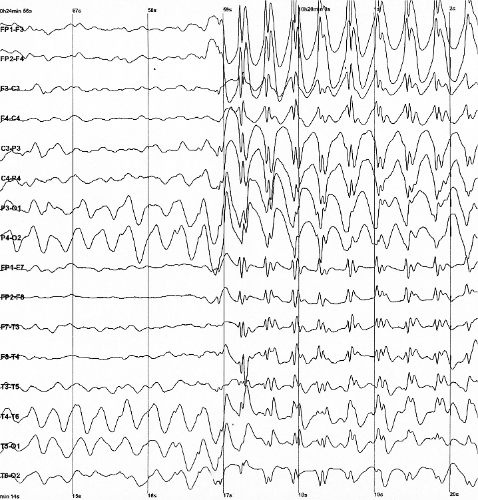
\includegraphics[width=0.6\textwidth]{eeg_example}
    \caption{Example of epileptic spikes monitored with \acs{eeg}}
    \label{fig:eeg_example}
\end{figure}

The number of electrodes used can range from a few dozen to hundreds. They are positioned on specific sections of the patient's head, therefore different electrodes monitor the activity of different areas of the brain. In this way, by looking at the \acs{eeg} and knowing the position of each electrode, the specialist can understand which areas of the patient's brain are involved in the seizure. The electrodes are identified based on whether they are placed on the left or right side of the head and also based on the lobe they are recording from (frontal lobes, temporal lobes, parietal lobes or occipital lobes). The \acs{eeg} monitoring captures several types of brain waves, which differ in the frequency. Specific ranges of frequencies are determined by particular moments of the day, situations and states of mind.

The \acs{eeg} is a very helpful tool for epilepsy diagnosis, but it can't show for certain the presence of epileptic seizures. In fact, despite the existence of typical signal patterns associated with epilepsy, usually epileptic seizures look very different on the \acs{eeg} depending on the patient: some seizures are recognizable thanks to the presence of typical spikes in the electrical signals; other seizures happen without showing any visible change in the \acs{eeg}. Therefore, we have reason to think that for some patients the seizure is "hidden" in the relations between signals behaviour, more than in the behaviour of each signal itself. Even when the change in the \acs{eeg} pattern is clear, it could involve only a subset of electrodes (partial seizures) or all the electrodes (generalized seizures), and it is difficult to determine if the disruption of the signal is actually caused by epilepsy or if it simply represents an 'abnormal' \acs{eeg}, which could happen without the presence of seizures.

%------------------------------------------------
% Problem definition
%------------------------------------------------

\section{Problem definition} \label{sec: problem_definition}
\paragraph{} The focus of this thesis is on the problem of seizure prediction, of which we are going to analyze three different cases in order to have a clearer and more complete idea of the machine learning models potentialities on epileptic seizures data.

The seizure prediction problem can be treated as a classification problem, whose aim is to predict a class associated with each sample. In the case of an \acs{eeg}, if we consider discrete instants of time (time steps), we can represent the \acs{eeg} information as a matrix $N \times F$, where the rows represent the $N$ electrodes and the columns represent the features associated with the $F$ time steps. So, for each of the $N$ electrodes, we have a sequence of $F$ values representing the amplitude over time. The task can be treated as a classification problem by associating each time step with a label or target, which represents the class of membership between \textit{seizure} and \textit{non-seizure}. This means that each time step is classified based on the presence or absence of an ongoing epileptic seizure in that instant. If we indicate with $x_t$ the set of signals features related to a single time step, we can say that each time step $t$ with features $x_t$ has an associated target $y_t$, which is equal to $1$ if there is an ongoing seizure and to $0$ otherwise. Thus considered, the seizure prediction problem becomes the task of predicting the class target $y_t$ related to the time step's features $x_t$.

\begin{figure}[htbp]
    \centering
    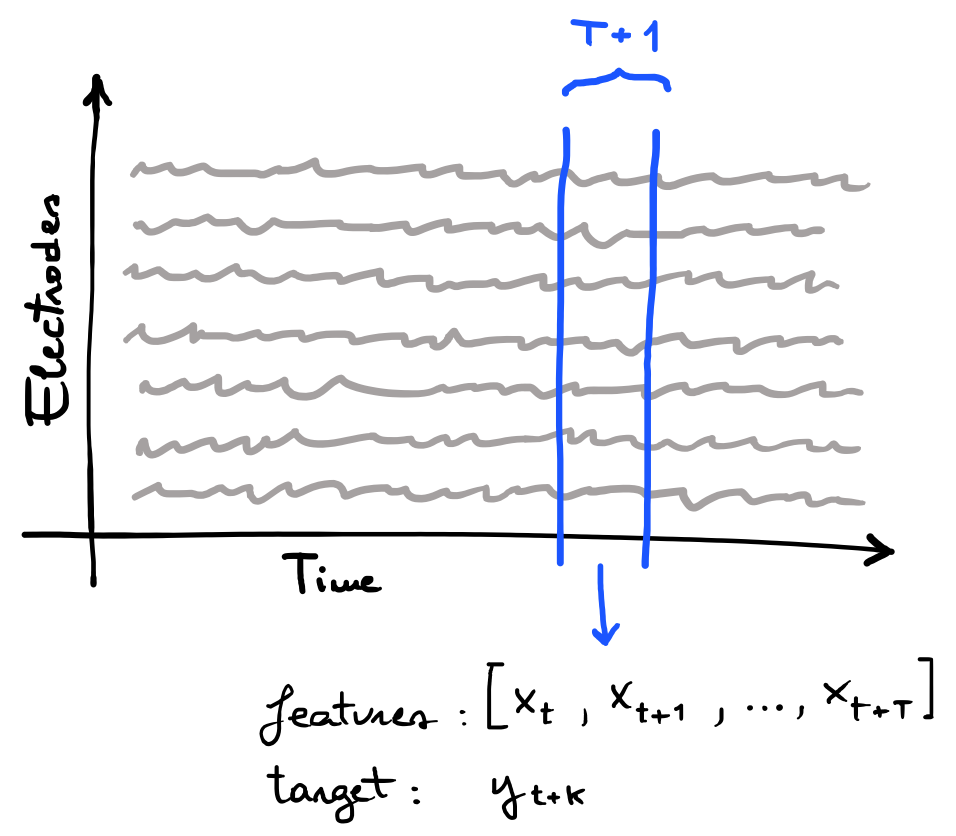
\includegraphics[width=0.6\textwidth]{problem_def}
    \caption{Problem definition}
    \label{fig:problem_def}
\end{figure}

Let's consider a time portion of $T+1$ discrete time steps in an \acs{eeg}: the portion will be characterized by a sequence of features $[x_t, x_{t+1}, x_{t+2}, ... , x_{t+T}]$, one for each time step $t$, representing the signals amplitude (measured in volts) in that instant. Let's imagine that the time portion is used to predict a single target $y_{t+k}$, which indicates whether the time step $t+k$ is part of an ongoing epileptic seizure or not. The described situation is illustrated in Figure \ref{fig:problem_def}. Considering this scenario, we can individuate three cases of study of the problem, depending on the value of the variables $T$ and $k$:
\begin{itemize}
    \item $T=0,\quad k=0$: in this case, the length of the time portion is equal to $1$ and the target corresponds to label of the single time step in the time portion (see Figure \ref{fig:problem_def1}). So at each time step $x_t$ is associated the target $y_t$ (as in the case described above). We can consider this case as a baseline scenario of the prediction problem, that is the detection based on a time step.\\
    \textsc{Example:} \quad$T=0, k=0\quad \Rightarrow{}\quad [x_3] \rightarrow{} y_3$
    \begin{figure}[h]
        \centering
        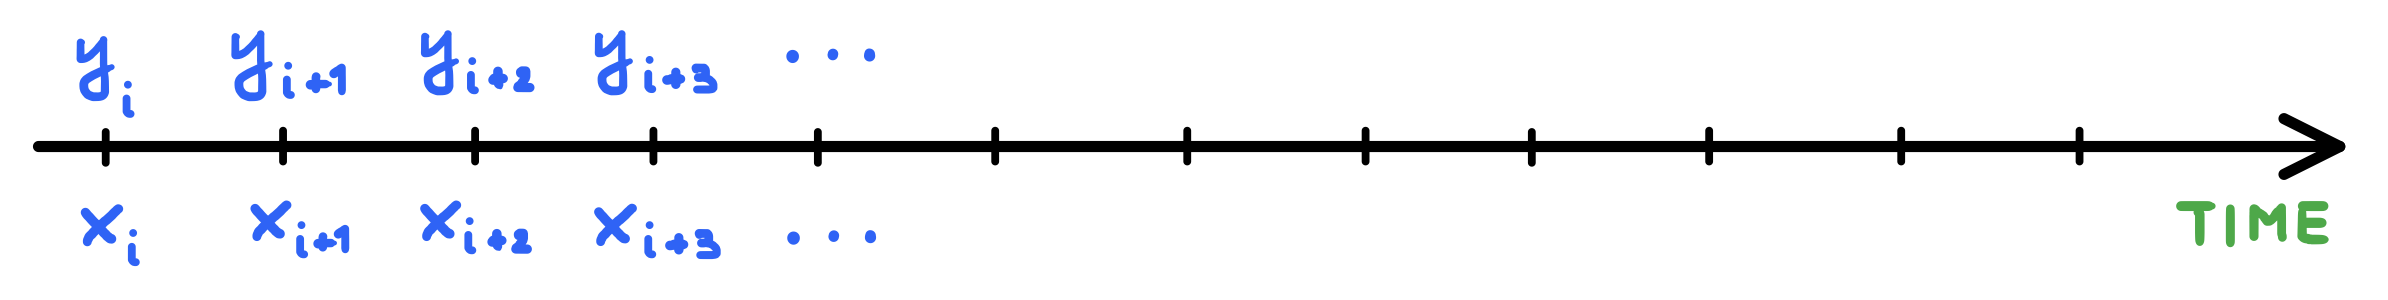
\includegraphics[width=0.8\textwidth]{problem_def1}
        \caption{Detection on a time step, representing the sample $x_i$ with target $y_i$}
        \label{fig:problem_def1}
    \end{figure}
    \item $T>0,\quad k=T$: in this case, the length of the time portion is greater that $1$, so a sample consists of a sequence of time steps, and the target is the label associated to the last time step of the sequence (see Figure \ref{fig:problem_def2}). So at each sequence $[x_t, x_{t+1}, ... , x_{t+T}]$ is associated the target $y_{t+T}$. This is still a borderline case of prediction, but with the addition of temporal dependencies between time steps, that is the detection based on a sequence of time steps.\\
    \textsc{Example:} \quad$T=5, k=5\quad \Rightarrow{}\quad [x_0, x_1, ..., x_5] \rightarrow{} y_5$
    \begin{figure}[h]
        \centering
        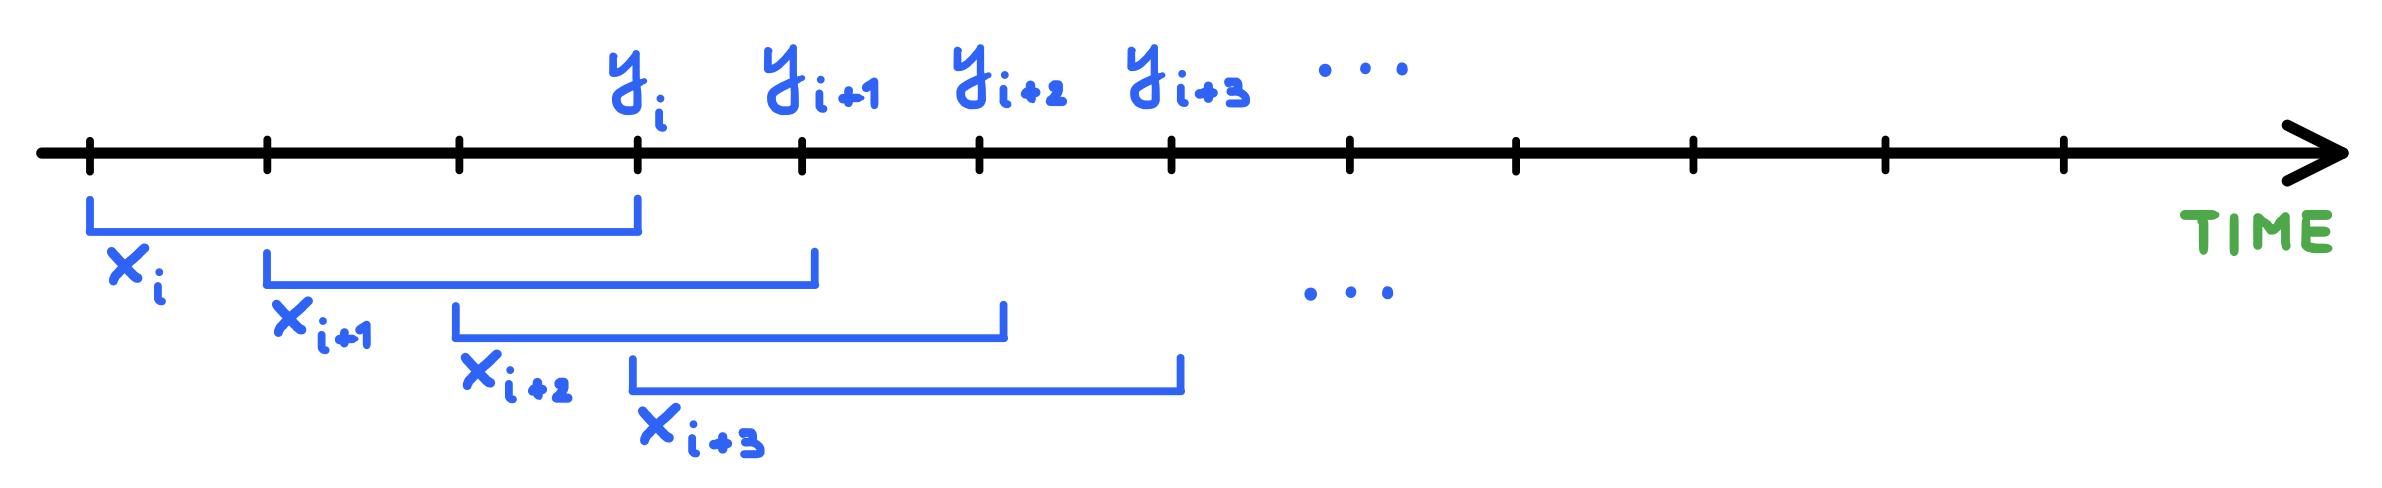
\includegraphics[width=0.8\textwidth]{problem_def2}
        \caption{Detection on a sequence, representing the sample $x_i$ with target $y_i$}
        \label{fig:problem_def2}
    \end{figure}
    \item $k>T$: in this case, we have a sequence of time steps whose target is associated to a time step that doesn't belong the sequence, but is forwards in time ($t>T+1$) (see Figure \ref{fig:problem_def3}). This means that at each sequence $[x_t, x_{t+1}, ... , x_{t+T}]$ is associated the target $y_{t+k}$, where $(t+k) > (t+T)$. This is the real prediction problem, since temporal dependencies are used to predict a time step some time in the future, so we are dealing with the prediction based on a sequence of time steps.\\
    \textsc{Example:} \quad$T=5, k=8\quad \Rightarrow{}\quad [x_0, x_1, ..., x_5] \rightarrow{} y_8$
    \begin{figure}[h]
        \centering
        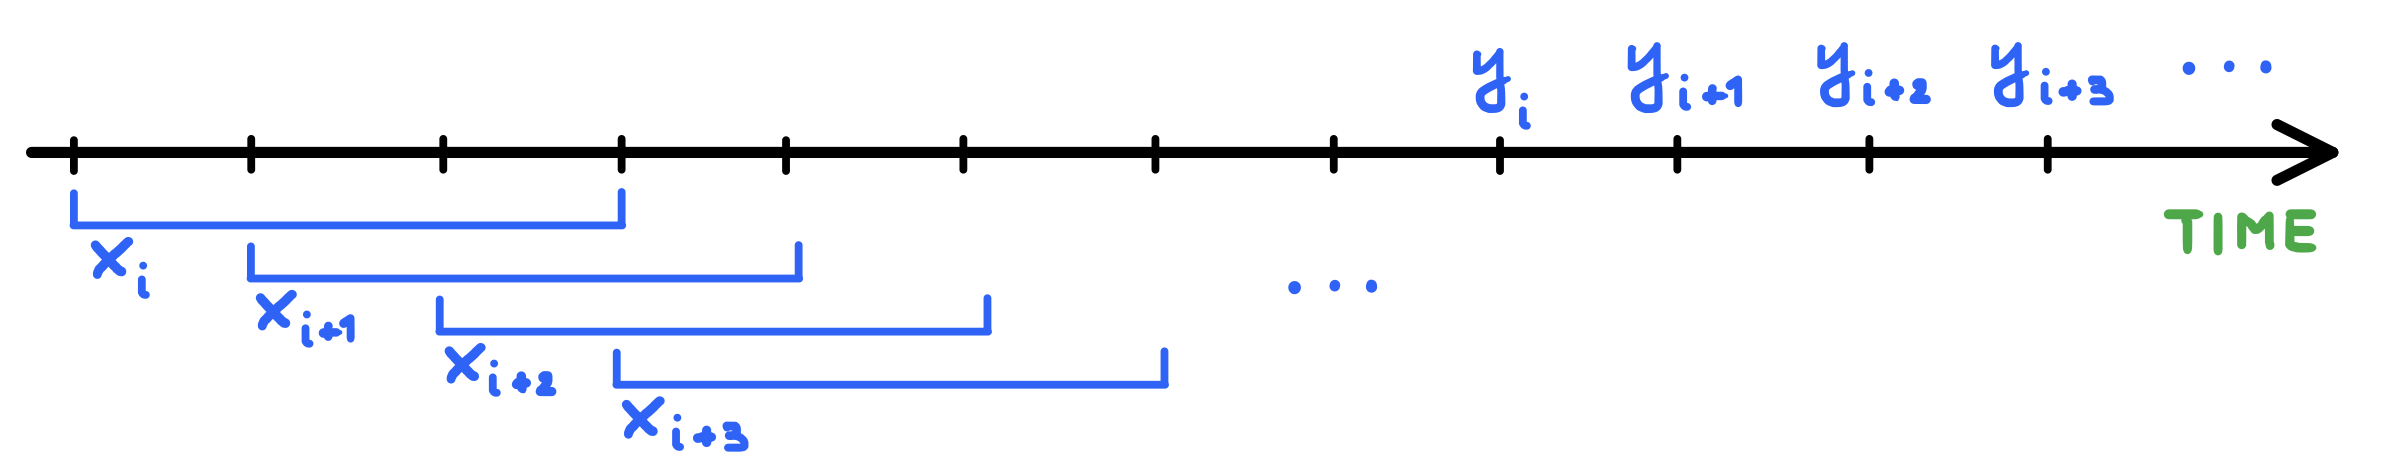
\includegraphics[width=0.8\textwidth]{problem_def3}
        \caption{Prediction on a sequence, representing the sample $x_i$ with target $y_i$}
        \label{fig:problem_def3}
    \end{figure}
\end{itemize}
The first two cases are examples of borderline cases of the prediction problem, that we define detection, since the target $y_{t+k}$ to predict is associated to a time step that is still inside the time window we look at to predict it ($k \leq T$). The third case, on the other hand, is a genuine prediction problem, since the target $y_{t+k}$ to predict is associated to a time step that is outside the time window we look at to predict it and it is forwards in time with respect to the time window ($k > T$). The difficulty of this last case is that we cannot look at the features $x_t$ in order to predict the target $y_t$, but we have to rely on information from previous time steps.

%------------------------------------------------
% Classification
%------------------------------------------------

\section{Classification} \label{sec: classification}
\paragraph{} The problem of epileptic seizure prediction can be identified as a classification task. Classification is the process of predicting the target associated with each sample in the data. In other words, the classification task consists in finding a mapping function from the input sample's features to the discrete output targets. This task is usually associated to data that can be assigned to a certain number of categories, which correspond to the targets to predict. When the data needs to be assigned to only two categories, we talk about binary classification. In this project, the problem of epileptic seizure (as described in Section \ref{sec: problem_definition}) can be considered a binary classification task, since we want to classify the time steps in two classes, which are the \textit{seizure} class and the \textit{non-seizure} class.

One of the most common methods to solve a binary classification task is logistic regression. Since the majority of models used in this project rely on logistic regression, we are going to use it as an example in order to provide a more complete description of the classification problem.

The logistic regression algorithm is used to estimate the probability that an instance belongs to a particular class \cite{OReilly:handsonML}. If the estimated probability is greater than a fixed threshold, which is commonly set to $0.5$, then the model assigns the instance to the positive class (in our case, \textit{seizure} class), otherwise it assigns the instance to the negative class (in our case, \textit{non-seizure} class). In this way, logistic regression can be used as a binary classifier.

Let's look at a very simple logistic regression model as an example: it computes the weighted sum of the input features $\mathbf{x}$ multiplied to the model parameter $\theta$ and it outputs the logistic of the result:
\begin{align}
    \hat{p} = h_{\theta}(\mathbf{X}) = \sigma\left(\theta^T \mathbf{x}\right)
\end{align}
The logistic $\sigma$ is a sigmoid function that generates a number between $0$ and $1$, representing the probability $\hat{p}$ that an instance $\mathbf{x}$ belongs to the positive class. The sigmoid function is illustrated in Figure \ref{fig:sigmoid} and it is mathematically defined as:
\begin{align}
    \sigma(t) = \frac{1}{1 + \exp{(-t)}}
\end{align}

\begin{figure}[htbp]
    \centering
    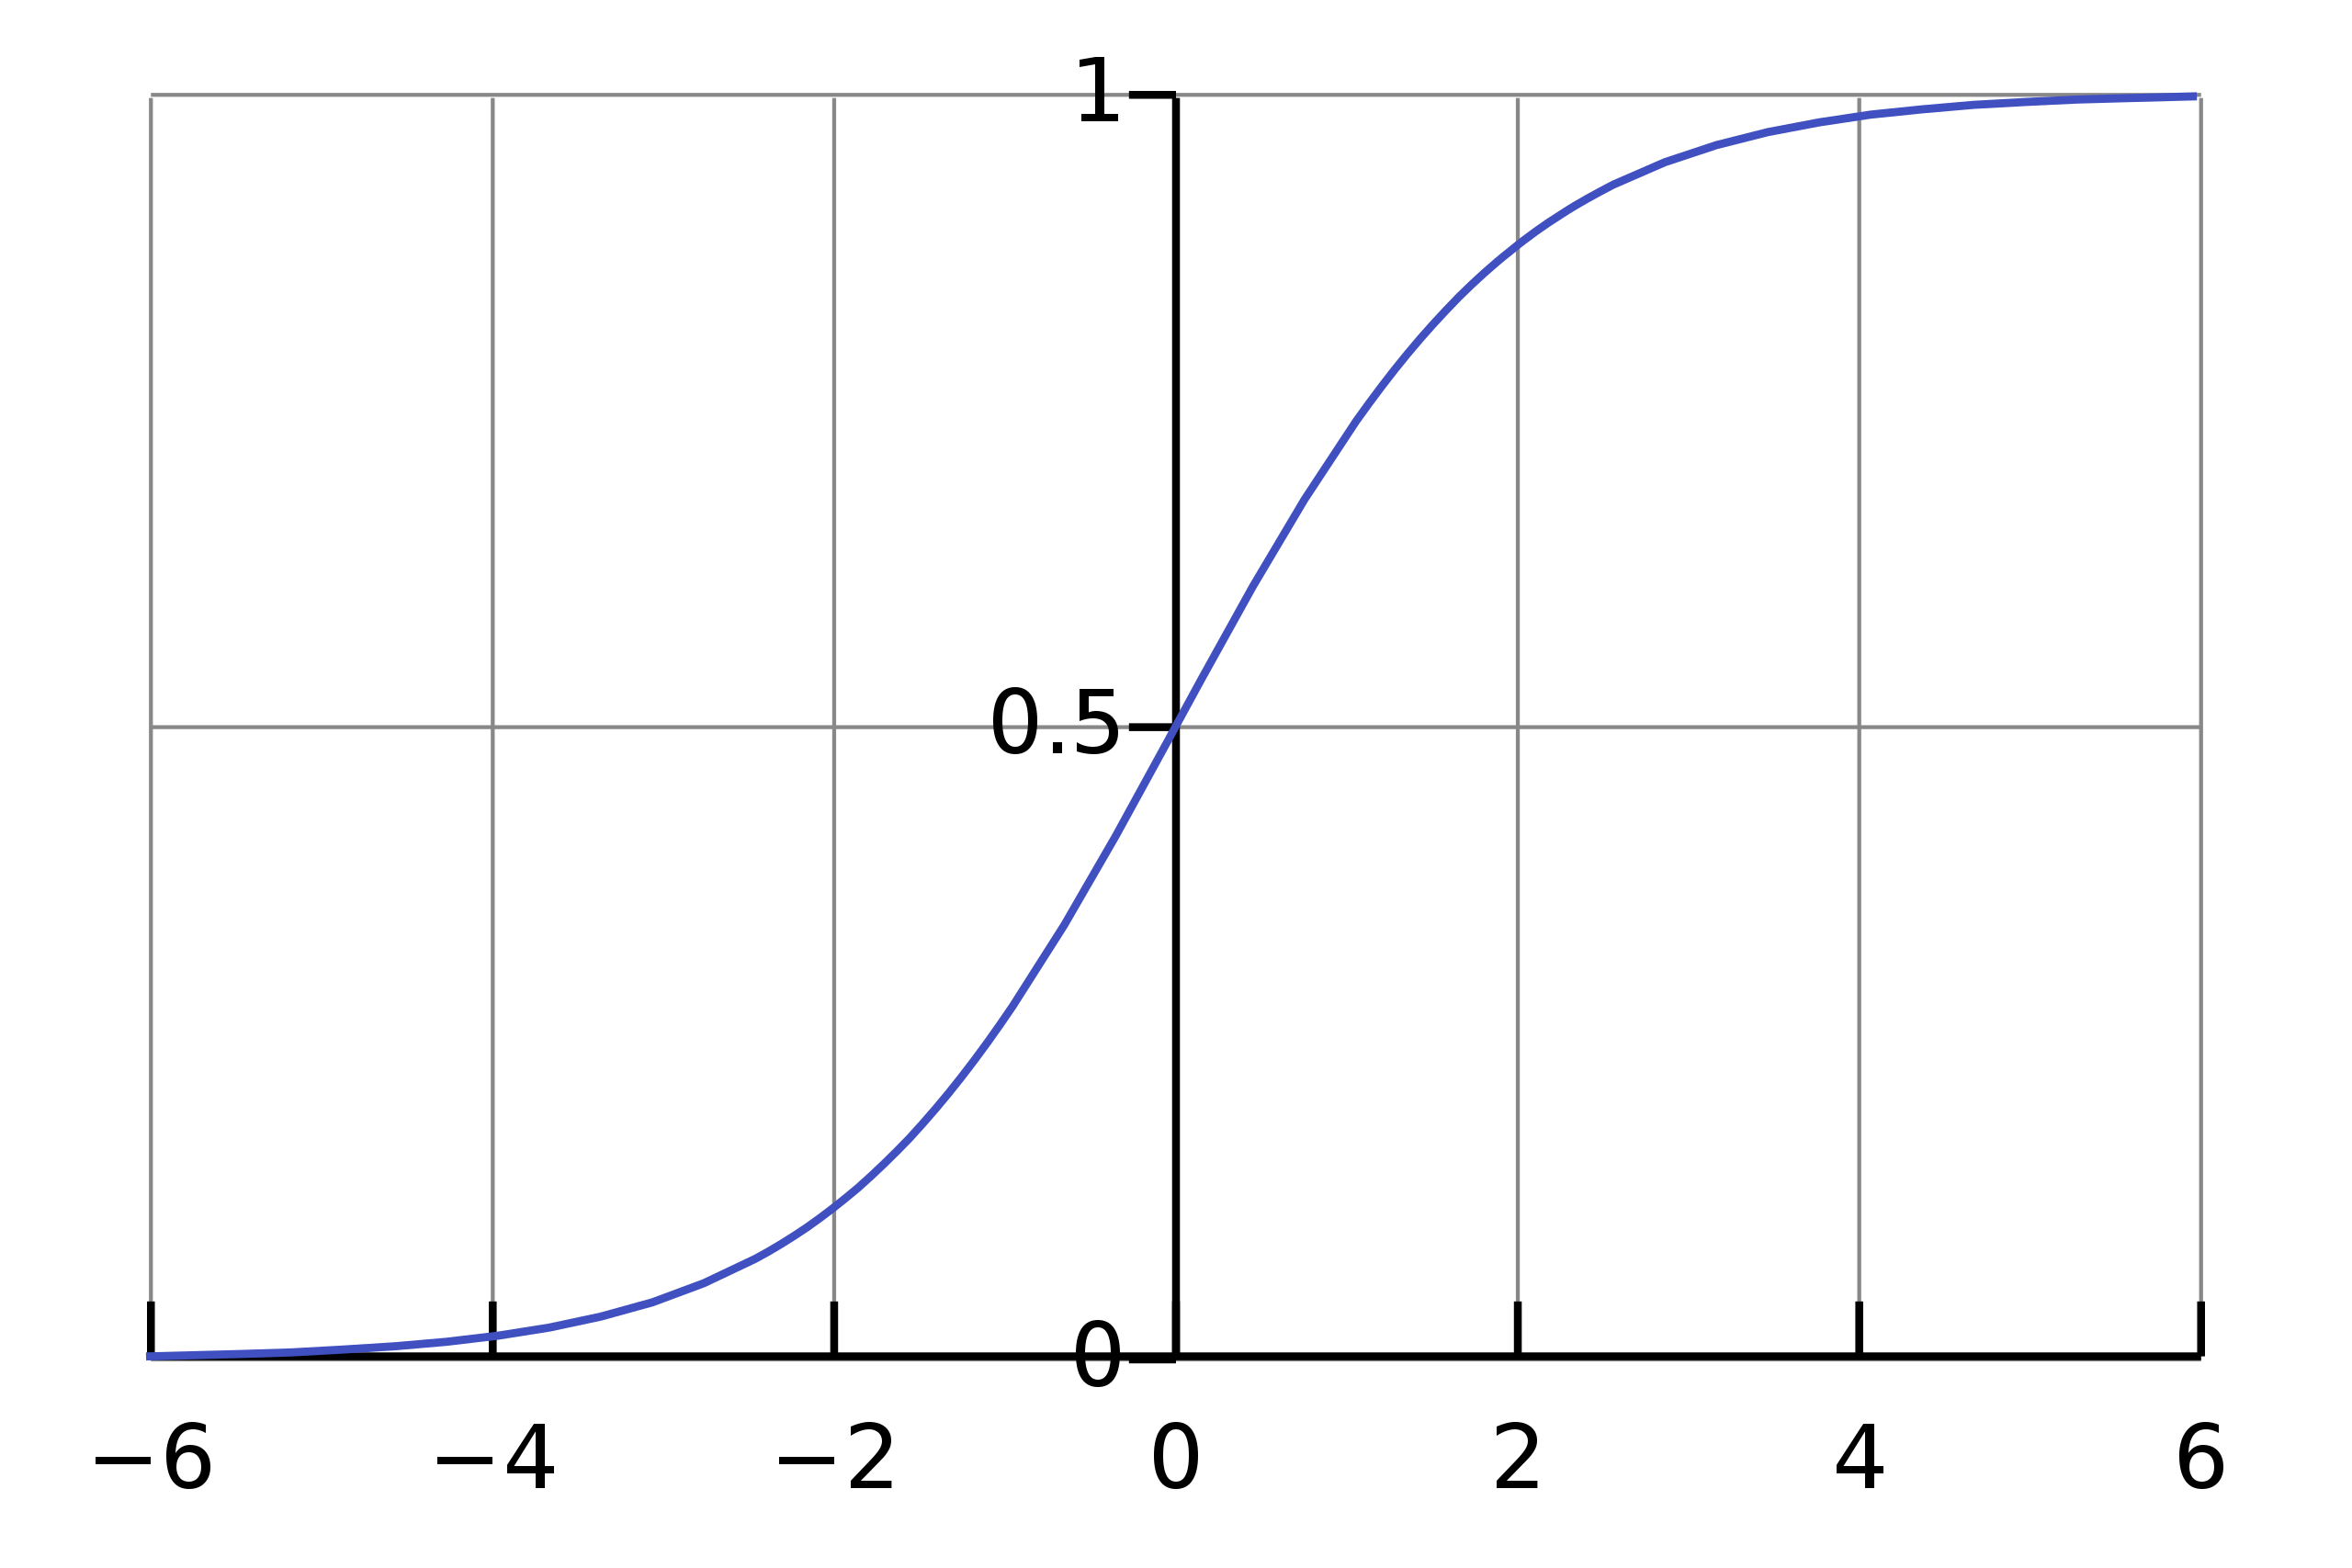
\includegraphics[width=0.6\textwidth]{sigmoid}
    \caption{Sigmoid function (from \textit{Wikipedia, the free encyclopedia})}
    \label{fig:sigmoid}
\end{figure}

The predictions $\hat{y}$ for the binary classifier can be easily obtained by applying the following equation to the estimated probability $\hat{p}$:
\begin{align}
    \hat{y} = \left\{\begin{array}{l}{0 \text { if } \hat{p}<0.5} \\ {1 \text { if } \hat{p} \geq 0.5}\end{array}\right.
\end{align}

The model parameter $\theta$ is trained in order to estimate high probabilities for positive instances and low probabilities for negative ones. In order to train it, we need a cost function that directs the model on the right track. For logistic regression algorithms, usually the most suitable cost function is the \textit{log loss}, since it captures exactly the aim of the classifier:
\begin{align}
    c(\theta) = \left\{\begin{array}{ll}{-\log (\hat{p})} & {\text { if } y=1} \\ {-\log (1-\hat{p})} & {\text { if } y=0}\end{array}\right.
\end{align}
$-\log (\hat{p})$ becomes higher and higher and tends toward infinity the more $\hat{p}$ get close to $0$, while it gets near to $0$ when $\hat{p}$ approaches $1$. $-\log (1-\hat{p})$ behaves in the opposite way, so it makes sense to use the first one for the positive class and the second one for the negative class. The cost function is applied to multiple training instances by computing the average cost over all the $n$ instances:
\begin{align}
    \textit{error } = -\frac{1}{n} \sum^{n}_{i=1}\left[y_i \log(\hat{p}_i) +
    (1 - y_i) \log(1 - \hat{p}_i)\right]
\end{align}
The log loss cost function is then used by an optimizer, for instance Gradient Descent or Root Mean Square Propagation algorithms, in order to update the model parameters accordingly. Usually, like in this project, the optimizer works on mini-batches, so the model parameters are updated after each mini-batch.

The algorithms that we studied in this work leverage this learning process, but instead of using such a simple model consisting of only one parameter, we used a set of more complex machine learning models and applied logistic regression to each of them to build several binary classifiers.

%------------------------------------------------
% Metrics
%------------------------------------------------

\section{Metrics} \label{sec: metrics}
\paragraph{} In order to evaluate the models, four metrics have been chosen, which are commonly used for binary classifiers: loss, accuracy, ROC-AUC and recall. The first two metrics are the most common performance measures for all the machine learning models.

\paragraph{Loss} The loss is the cost function evaluated on a particular set of data. In our case, we used the log loss (already described in Section \ref{sec: classification}) for deep learning models and the mean squared error (\acs{mse}) loss for classic machine learning models as cost functions. The \acs{mse} loss, also called Brier score, is the mean squared difference between the predicted probability and the actual target. The \acs{mse} loss takes values between 0 and 1 and it suggests whether the predictions are well calibrated. Its formula is:
\begin{align}
    \textit{MSE loss}=\frac{1}{n} \sum_{i=1}^{n}(\hat{p}_{i} - y_{i})^{2}
\end{align}
where $n$ is the number of samples, $\hat{p}_i$ is the predicted probability of sample $i$ and $y_i$ is the target of sample $i$.

\paragraph{Accuracy} The accuracy is simply the ratio of correct prediction, which in a binary classifier is represented by the number of true prediction (true positive and true negative) over the total number of predictions:
\begin{align}
    \textit{acc } = \frac{(TP + TN)}{(TP + TN + FP + FN)}
\end{align}
where \textit{TP} = true positive, \textit{TN} = true negative, \textit{FP} = false positive, \textit{FN} = false negative.

\paragraph{Recall} The recall, also called sensitivity or true positive rate, is the number of positive instances correctly classified over the total number of positive instances:
\begin{align}
    \textit{recall } = \frac{(TP)}{(TP + FN)}
\end{align}

\paragraph{ROC-AUC} The receiver operating characteristic curve (\acs{roc} curve) is a plot of the true positive rate (recall) against the false positive rate (shown in Figure \ref{fig:roc_auc}):
\begin{align}
    \textit{TPR } = \frac{(TP)}{(TP + FN)} \qquad\qquad \textit{FPR } = \frac{(FP)}{(FP + TN)}
\end{align}
The false positive rate is the number of negative instances incorrectly classified as positive over the total number of negative instances.
\begin{figure}[htbp]
    \centering
    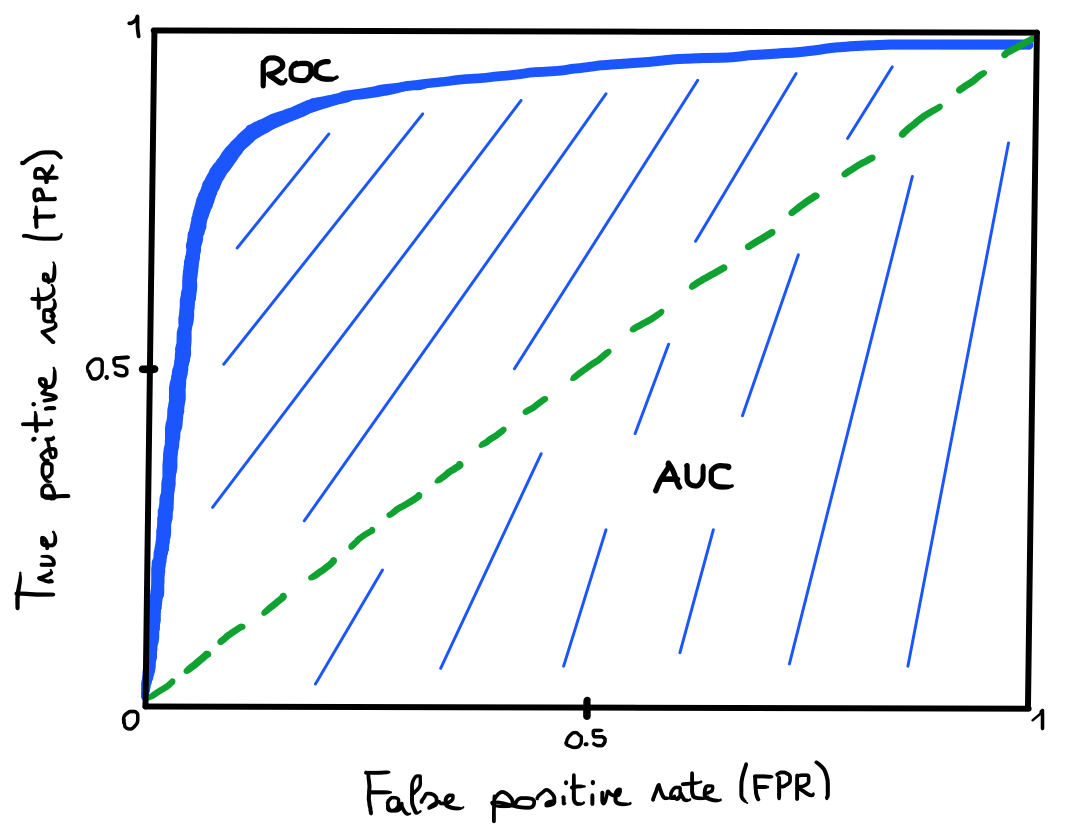
\includegraphics[width=0.6\textwidth]{roc_auc}
    \caption{\acs{roc} curve and respective \acs{auc}}
    \label{fig:roc_auc}
\end{figure}

The \acs{roc} curve represents a plot of TPR and FPR at different classification thresholds: if we lower the threshold, the classifier predicts more items as positive, so both TPR and FPR increase. In order to find the best classification threshold, we need to find a tradeoff between TPR and FPR, trying to obtain a higher TPR as possible and a lower FPR as possible (looking at the curve, we need to find the point that is closest to the upper left corner). For this purpose we can rely on the \textit{area under the \acs{roc} curve} (\acs{auc}), which provides a performance measure for different classification thresholds. The ROC-AUC ranges from 0 to 1 and its value represents the quality of the classifier predictions. A perfect classifier has \acs{auc} = 1, while a completely random classifier has \acs{auc} = 0.5.

%------------------------------------------------
% Classic machine learning models
%------------------------------------------------

\section{Classic machine learning models} \label{sec: classic_ml_models}
\paragraph{} Machine learning models are able to perform a specific task efficiently, without the need of explicit instructions, but relying uniquely on the patterns and features they learn from data. Giving the nature of this project's problem and the type of data we are working on, all the models that have been used have been trained in a supervised manner; this means that the training data fed to the algorithm includes the labels. In the case of a classification task, the training data consist of both the data features and the respective classes of membership, so that the model can learn from examples and discover patterns that allow it to make good predictions on new data.

In this section we are going to describe the classic machine learning algorithms that have been used, leaving the deep learning models (neural networks) for the next section.

\subsection{Random forest}
\paragraph{} A random forest is an ensemble of decision trees, which are machine learning algorithms able to perform both classification and regression \cite{OReilly:handsonML}. To understand how a random forest works, we first need to say a few words about decision trees.

A decision tree is a model represented as a tree in graph theory, with a root node, internal vertices, leaf nodes and edges between them. Each node can be seen as a decision unit: it contains a boolean expression based on some input features and it makes decisions based on this condition. The leaf nodes make and exception since, for classification tasks, each of them correspond to a different class. The classification of a single input instance, then, works as follows: starting from the root node, each node evaluate its boolean expression on one (or multiple) instance's feature and, depending on whether the condition is \textit{True} or \textit{False}, the path to follow continues on the left or right child of that node. The process goes on until a leaf node is reaches and the instance is finally assigned to the class corresponding to that leaf node. Figure \ref{fig:decision_tree} shows and example of a decision tree applied to the famous Iris dataset for classification. In that case, the features used by nodes to create a condition are at first the petal length and then the petal width. The three leaf nodes correspond to the tree classes: setosa, versicolor and virginica. The \textit{gini} attribute assigned to each node measures its impurity, which depends on the class distribution of the instances to which the node is applied. If $gini = 0$, then the node is pure, meaning that all the instances to which it is applied belong to the same class. If all the leaf nodes' \textit{gini} attribute is equal to zero, then the decision tree has perfectly classified all the instances.
\begin{figure}[htbp]
    \centering
    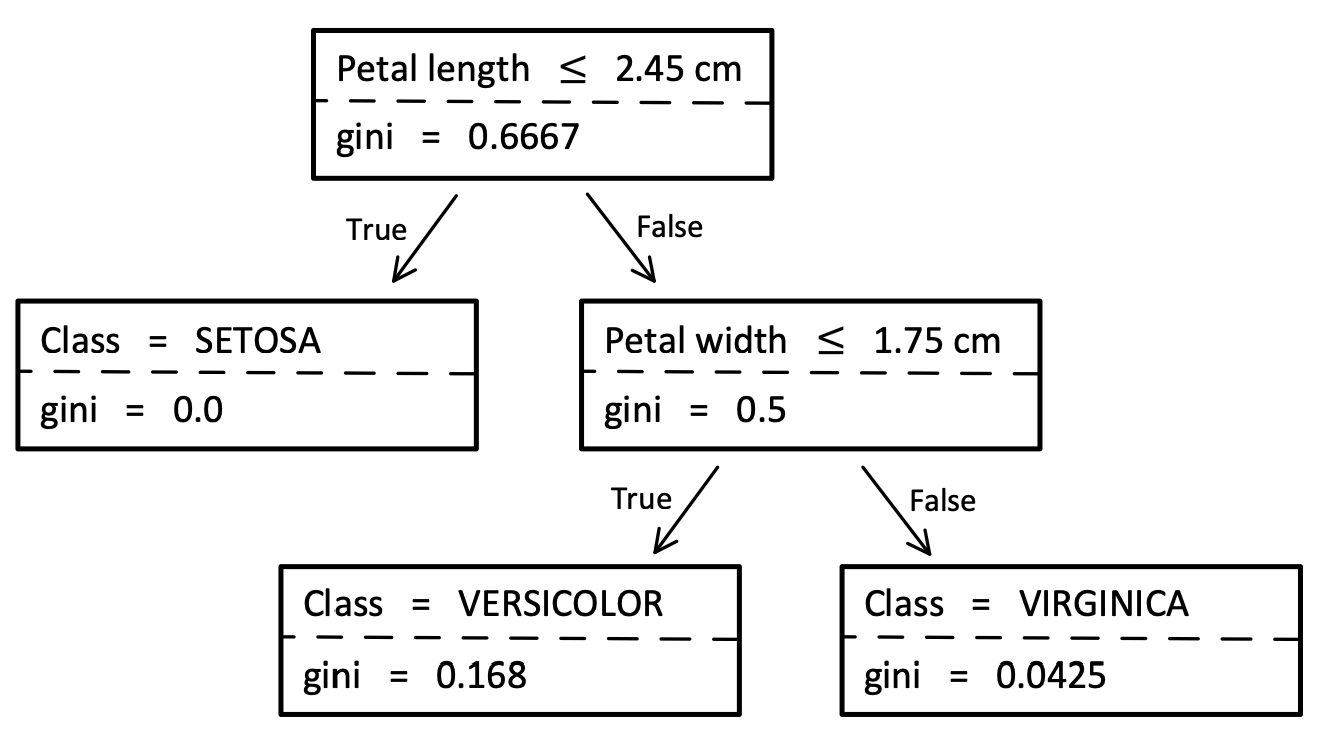
\includegraphics[width=0.7\textwidth]{decision_tree}
    \caption{Example of decision tree applied to the famous Iris dataset for classification}
    \label{fig:decision_tree}
\end{figure}

When the final prediction is computed using an ensemble of decision trees, we talk about random forest. In a random forest, $k$ different decision trees are trained in parallel on different random subsets of the training set. The sampling of the data can be performed with replacement (\textit{bootstrapping}), like in this project, or without replacement. Both methods allow training instances to be selected multiple times for different decision trees, but, when using bootstrapping, the same instance could be selected multiple times also for the same decision tree. Once all the decision trees have been trained, the random forest prediction is computed by aggregating the predictions of all its decision trees. Typically the statistical mode is used as aggregation function, but the average can be used as well. A random forest can be regularized by setting the number of decision trees to use and their maximum depth.

In general, random forest algorithms work better than decision trees and are less prone to overfitting. The reason is the greater tree diversity: in addiction to the data sampling, when splitting a node during the construction of the tree, the split is chosen no longer as the best among all features, but as the best among a random subset of the features.

\subsection{Gradient boosting}
\paragraph{} Gradient boosting (tree-based) is very similar to random forest, as it is itself an ensemble of decision trees. Differently from random forest, in gradient boosting the decision trees are trained in a sequential way, one at a time, and each one tries to correct the errors made by its predecessor. In particular, each new decision tree is fitted on the residual errors made by the previous one. Therefore, while the first decision tree of the sequence will fit the instances $\mathbf{X}$ and the targets $\mathbf{y}$, the second decision tree will fit $\mathbf{X}$ and the residual errors $y_1 = \mathbf{y} - \hat{y}_1$, where $\hat{y}_1$ are the predictions made by the first decision tree on $\mathbf{X}$. Likewise, the third decision tree will fit $\mathbf{X}$ and the residual errors $y_2 = y_1 - \hat{y}_2$, where $\hat{y}_2$ are the predictions made by the second decision tree on $\mathbf{X}$, and so on. So we can consider gradient boosting as a gradient descent algorithm.

Usually gradient boosting have better performance with respect to random forest, but, since decision trees are not trained independently, it is more prone to overfitting.

\subsection{Support vector machine}
\paragraph{} \acf{svm} is a very powerful machine learning algorithm able to perform both linear and non-linear classification and regression \cite{OReilly:handsonML}. It is a binary classifier, but it can be used also as a multiple-class classifier. In order to classify data, the \acs{svm} represents the instances as points on a decision surface and divides them through a decision boundary that is placed in the middle of the largest possible gap between the two classes' instances (positive and negative class). In other words, if we imagine the data projected in a 2-dimensional space, the \acs{svm} tries to find a line able to separate the positive and negative instances staying as far away as possible from the closest instances. This situation is illustrated in Figure \ref{fig:svm_line}, where the two group of instances, belonging to the blue and green classes, are divided by the red line. The boundary generated by the \acs{svm} is placed as far as possible from the instances, trying to maximize the distance $w$ from the nearest instances. In this way, in case we made a small error in the location of the boundary, we have a margin of error that prevents a misclassification. The instances that lie on the edges of the decision boundary's margins are called \textit{support vectors} (in Figure \ref{fig:svm_line} they are represented as filled circles). The position of the support vectors completely determines the max-margin decision boundary and the distance between support vectors of different classes determine the width of the optimal boundary’s margins.
\begin{figure}[htbp]
    \centering
    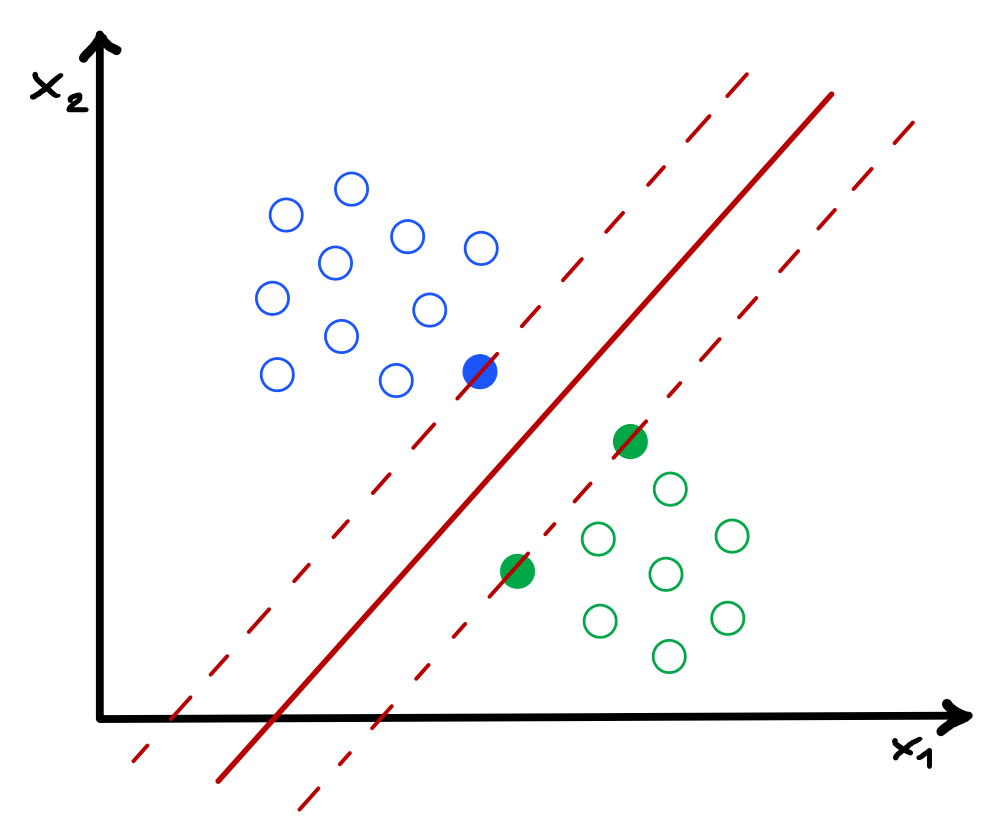
\includegraphics[width=0.4\textwidth]{svm_line}
    \caption{Example of \acs{svm} decision boundary for data classification}
    \label{fig:svm_line}
\end{figure}

In the general case with $d$-dimensional data, \acsp{svm} find a ($d-1$)-dimensional hyperplane such that the margin of separation between the two classes is maximized.

If the data points are linearly separable, the \acs{svm} is able to construct two parallel hyperplanes that separate the data points in the two respective classes. The hyperplanes can be respectively described by the two equations:
\begin{align}
    &\vec{w} \cdot \vec{x}^{+}-b=1 \\
    &\vec{w} \cdot \vec{x}^{-}-b=-1
\end{align}
The distance between the two hyperplane is $\frac{2}{\|\vec{w}\|}$, so, in order to maximize the distance between them, we want to minimize $\|\vec{w}\|$, while avoiding margin violations (\textit{hard margin}) or limiting them (\textit{soft margin}).

Hard margin can be used for problems where the data points are linearly separable. In this case, the max-margin hyperplane is completely determined by those data points which are nearest to it and we want to prevent data points from falling into the margin. To reach this result, we can use the following objective function, subjected to the following constraints:
\begin{align}
    &\text{objective function }= \min \frac{1}{2}\|\vec{w}\|^2 =  \min \frac{1}{2} w^{T} w\\
    &\text{constraints }= \left\{\begin{array}{ll}{\text{if } y=1 :} & {w^{T} x+b \geq 1} \\ {\text{if } y=0 :} & {w^{T} x+b <-1}\end{array}\right.
\end{align}
These constraints guarantee that each point lies on the correct side of the margin.

In some cases, the problem can be non-linear and therefore not solvable with hard-margin; in other cases, the problem can be linear, but we would like a general solution that takes into account the presence of some errors in the data. In these situations, soft-margin can be used in place of hard-margin. Soft-margin \acsp{svm} allow some exceptional data points to fall into the margin or to lie on the wrong side of the margin. Soft-margin \acs{svm} introduces two new parameters: $\varepsilon_i$ represents the distance of $x_i$ from his true class margin hyperplane; $C$ is a parameter that allows to control better the softness of the margin, defining the tradeoff between the objective and the constraints. If $C$ is very big, the \acs{svm} becomes very rigid and behaves similarly to hard-margin; on the other hand, if $C$ is very small, the \acs{svm} imposes a smaller penalization for misclassified samples. Soft-margin is defined by the following objective function, subjected to the following constraints:
\begin{align}
    &\text{objective function }= \min \frac{1}{2} w^{T} w + C \sum^{n}_{i=1} \varepsilon_i\\
    &\text{constraints }= \left\{\begin{array}{lll}{\text{if } y=1 :} & {w^{T} x+b \geq (1 - \varepsilon_i)} \\ {\text{if } y=0 :} & {w^{T} x+b < (-1 + \varepsilon_i)} \\ {\text{for all } i :} & {\varepsilon_i \geq 0}\end{array}\right.
\end{align}
Figure \ref{fig:svm_formulas} shows a geometric representation of the parameters and formulas just presented.
\begin{figure}[htbp]
    \centering
    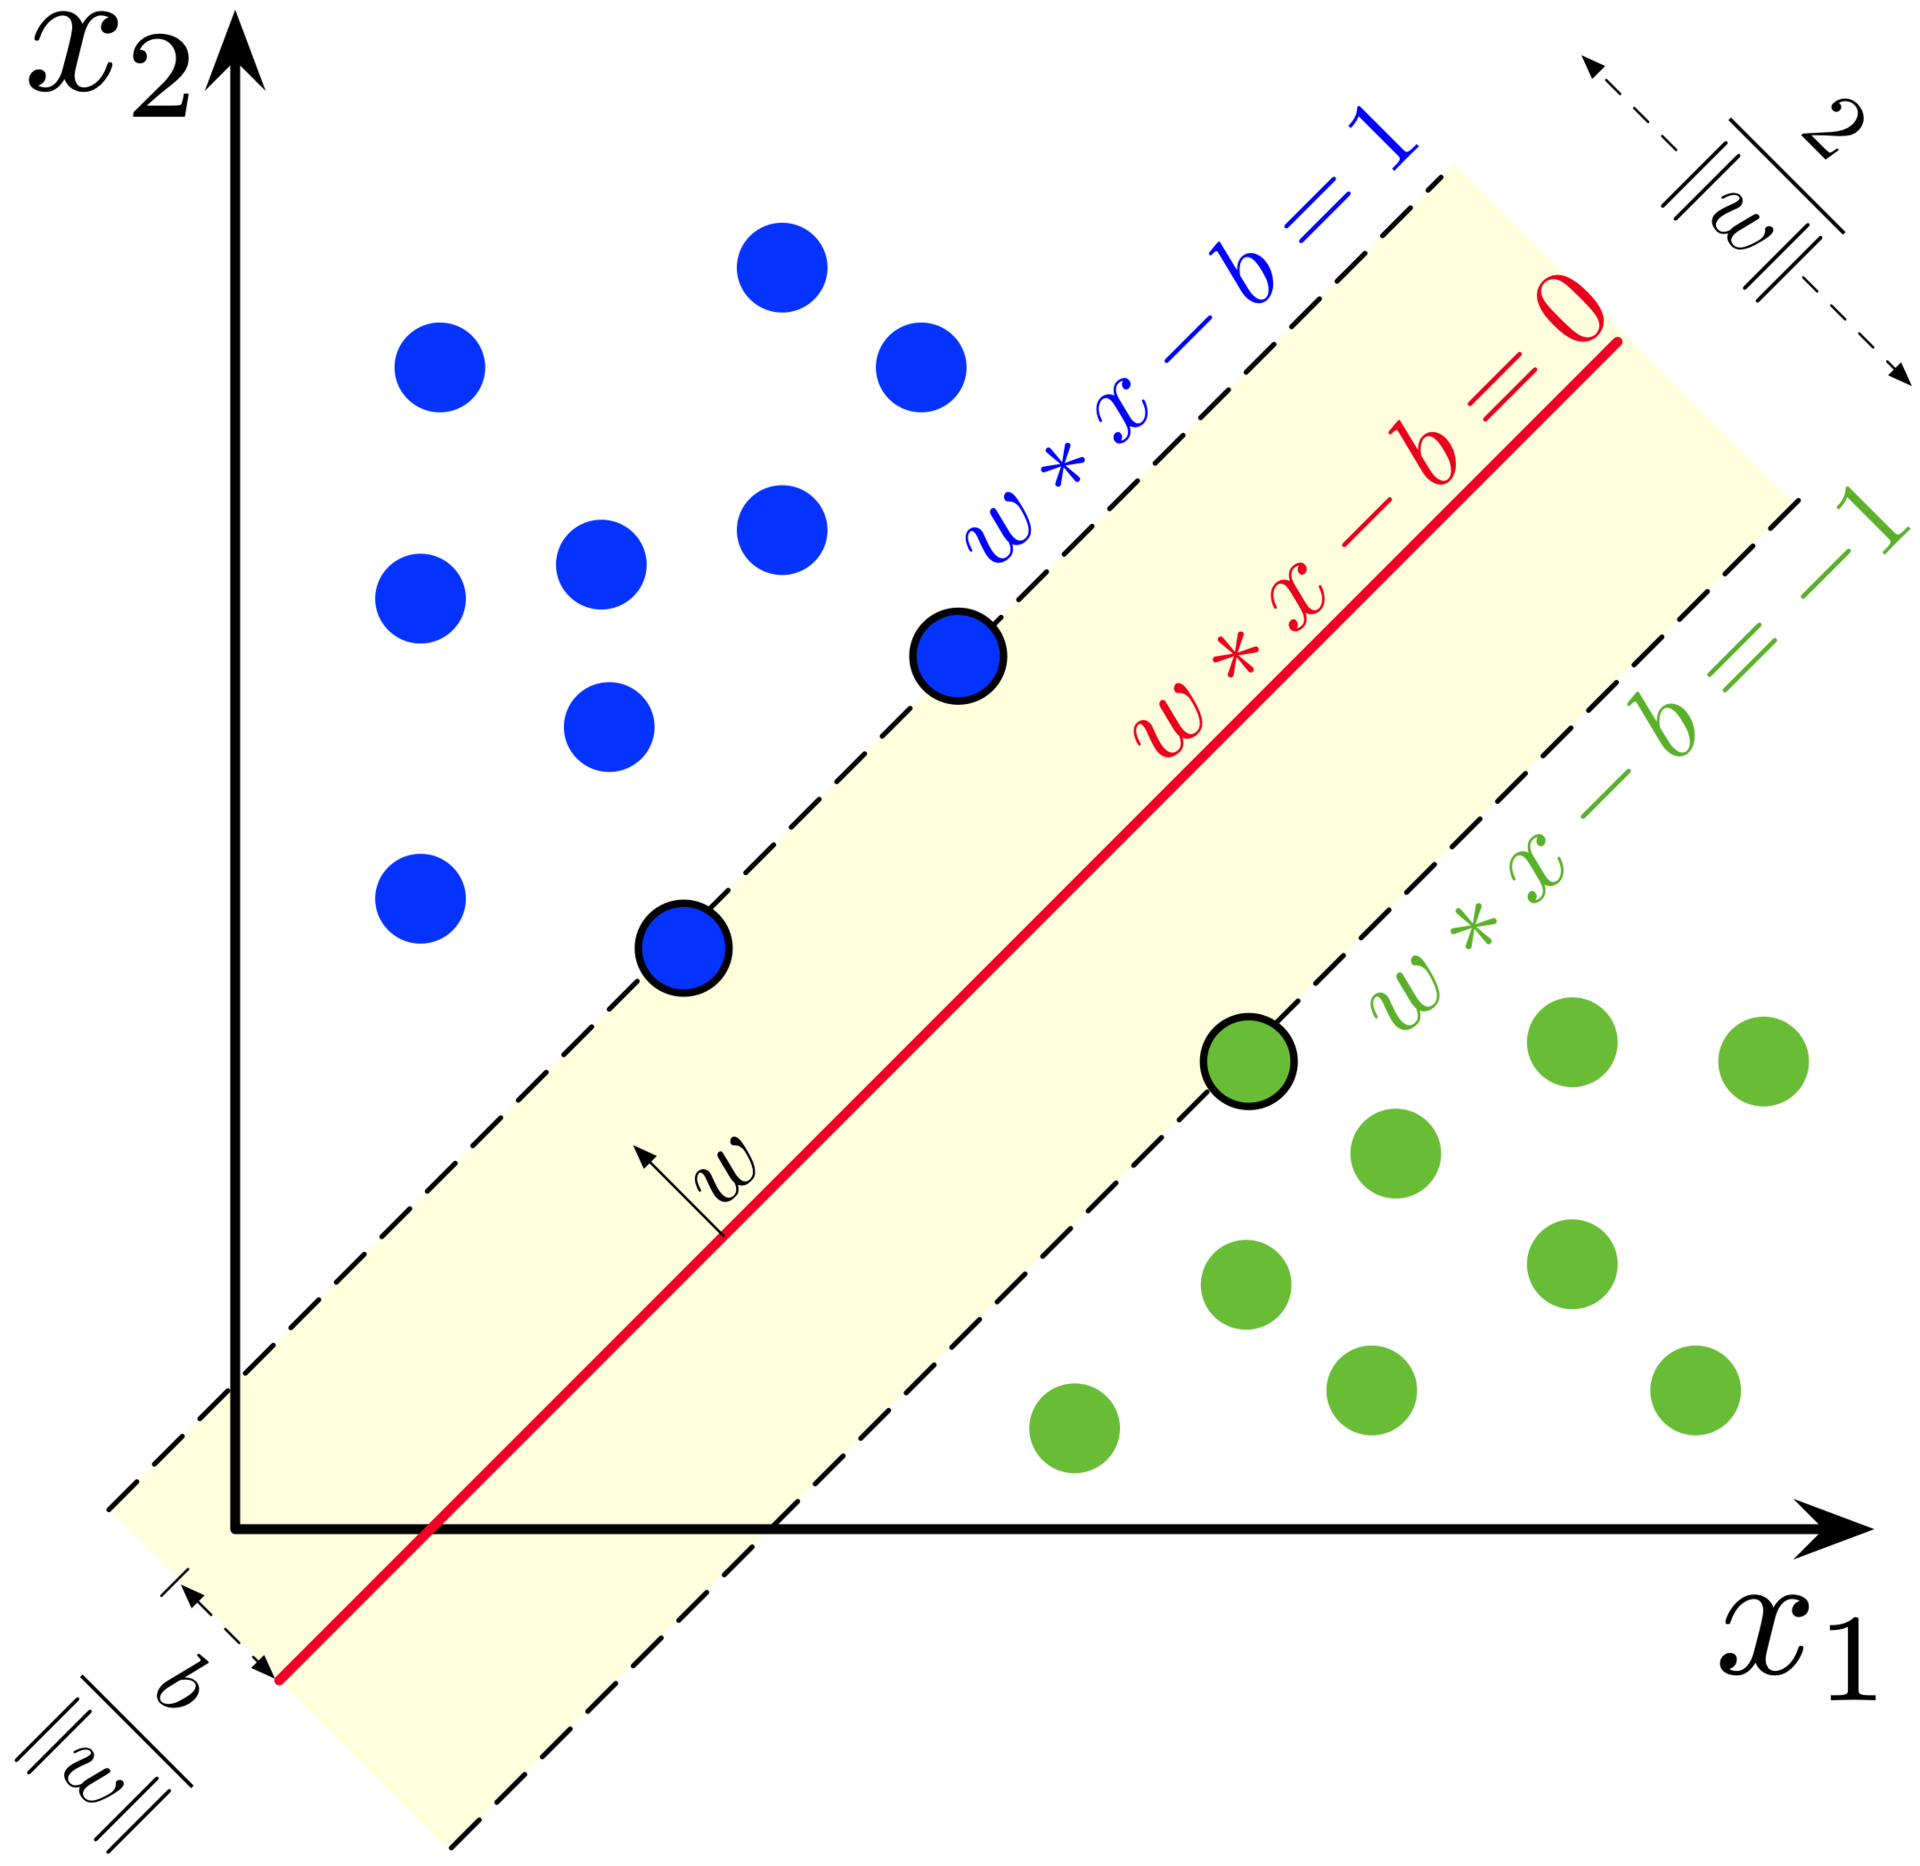
\includegraphics[width=0.4\textwidth]{svm_formulas}
    \caption{Geometric representation of \acs{svm}'s equations}
    \label{fig:svm_formulas}
\end{figure}

When data are not linearly separable, we can still use \acs{svm} in two ways: we can simply use soft-margin and permit some tolerance in presence of errors, or we can rely on a kernel function $K(a, b)$. A kernel function allows the \acs{svm} to lead the data points to a situation where they are linearly separable again. Indeed, the data can be mapped to a higher-dimensional feature space, where they are linearly separable by an optimal hyperplane. A feature map is the function that maps the data points to an higher-dimensional feature space: the function $\phi(x_i)$ maps every $x_i$ to the new feature space:
\begin{align}
    <\phi(a), \phi(b)>
\end{align}
The increase of space's dimensions can be computationally expensive, due to the computation of all the additional features. To avoid an high-cost computation, we can use the \textit{kernel trick}: applying a kernel function allows to compute the dot product of weights in the lower-dimensional space instead of in the higher-dimensional space:
\begin{align}
    <\phi(a), \phi(b)> = K(a, b)
\end{align}
The trick consists in expressing the problem just in function of the dot products, without the need to know the entire mapping to the new feature space. Actually, a kernel is a function that is able to compute the dot product $\phi(a)^T \phi(b)$ based only on the original vectors $a$ and $b$, without the need to compute the transformation $\phi$ on the vectors. Figure \ref{fig:svm_nonlinear} shows an example of a non-linear separable problem that could be solved by mapping data to a higher-dimensional space.
\begin{figure}[htbp]
    \centering
    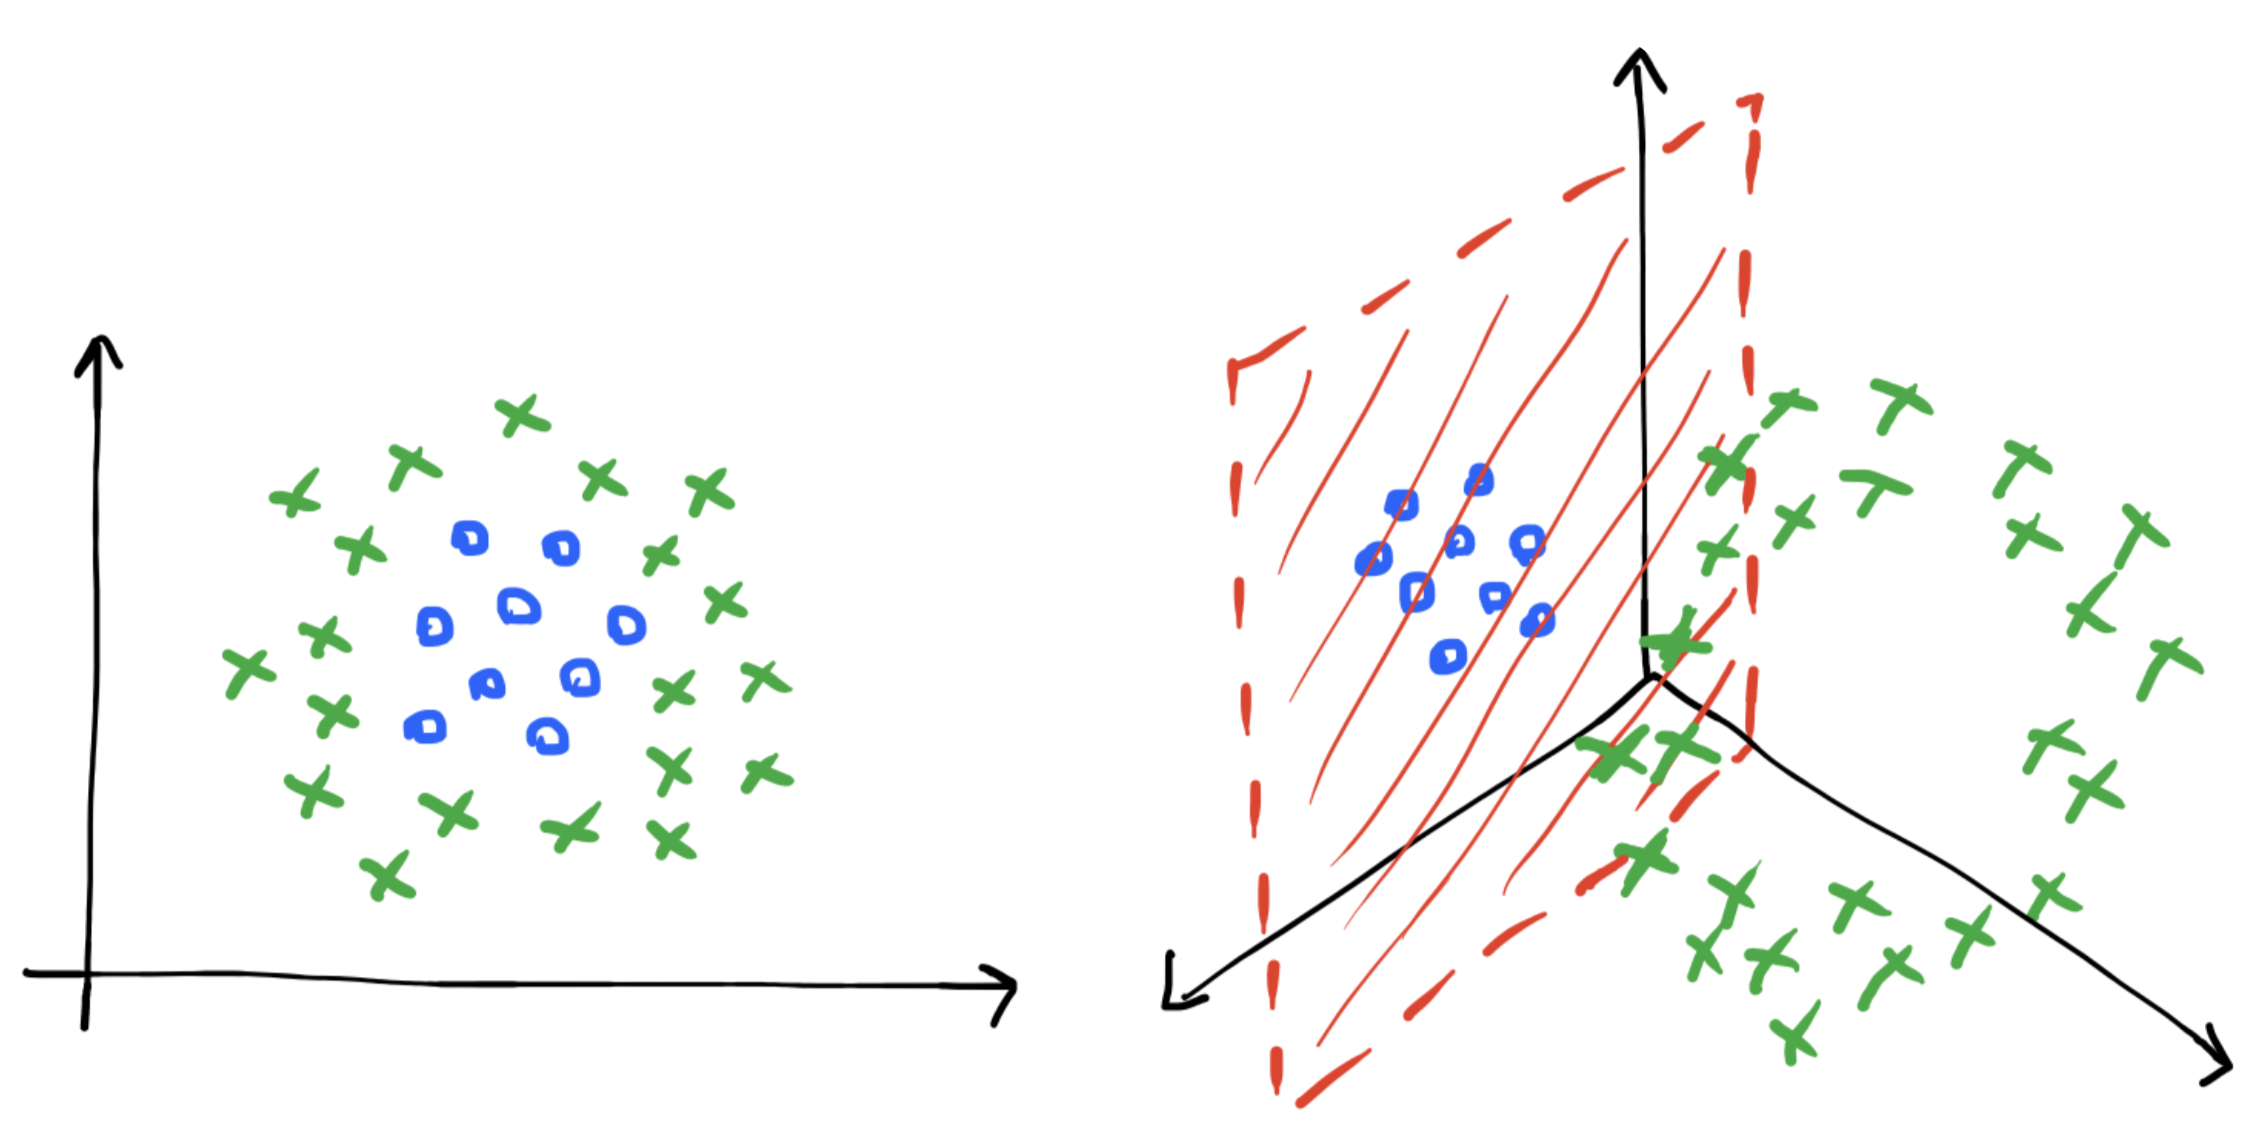
\includegraphics[width=0.6\textwidth]{svm_nonlinear}
    \caption{Example of a non-linear separable problem solved in a higher-dimensional space}
    \label{fig:svm_nonlinear}
\end{figure}

A frequently used kernel is the Gaussian \acf{rbf} kernel. This kernel generates new features by measuring the distance between the support vectors and all other instances: the function value decreases as the distance from the support vectors grows, so it can be considered a similarity measure. Through Gaussian \acs{rbf} kernel, the input vector is mapped to an infinite vector and then normalized by dividing each component by the vector’s length. The Gaussian \acs{rbf} kernel is defined by the equation:
\begin{align}
    K(a, b) = \exp \left(-\frac{\|a - b\|^{2}}{2 \sigma^{2}}\right) = \exp \left( -\gamma \|a - b\|^{2} \right)
\end{align}
The hyperparameter $\gamma = \frac{1}{2 \sigma^{2}}$ can be used as regularization term, since it controls how strict the decision boundary is by determining a strong sharpness if $\gamma$ is big (if $\sigma$ is small) and a weak sharpness otherwise (if $\sigma$ is big). So if the \acs{svm} is overfitting, $\gamma$ should be reduced, and if it is underfitting, $\gamma$ should be increased.

The kernel trick can be used together with the soft-margin in order to reach good performance and better generalization.

%------------------------------------------------
% Deep learning models
%------------------------------------------------

\section{Deep learning models} \label{sec: dl_models}
\paragraph{} Deep learning is a subfield of machine learning that differentiate itself for the specific type of models that it uses in order to learn a certain task. Deep learning models use a hierarchical representation of the features in order to make predictions \cite{Nvidia:dl}. Like other machine learning algorithms, deep learning models automatically extract common patterns found in the data, which become the crucial features to be used in the classification or regression process. The difference with standard machine learning methods is in the way the features are gathered. Deep learning models organize the feature identification in a hierarchical way, by extracting multiple layers of non-linear features to be used for making predictions. The \textit{deep} hierarchy of non-linear features allows the model to learn more complex features with respect to standard machine learning algorithms. The most common deep learning models, which make use of a hierarchical representation of the features, are \textit{artificial neural networks}.


\subsection{Artificial neural networks}
\paragraph{} Artificial neural networks, or simply neural networks (\acsp{nn}), are very powerful and versatile models that are inspired by human neural networks: the structure of artificial neural networks is comparable to the one of our brain, which has neurons and connection between them to transmit electrical impulses. Similarly, artificial neural networks are composed by several neurons which are the computational cores of the model and which transmit the processed information to each other.

Neural networks organize the neurons in layers: the input layer is represented by the input data, the output layer is the last one that process data and returns the result of the entire model, while all the layers in between are called \textit{hidden layers} and, in addition to transforming the data, they send the processed information to the next layer. Figure \ref{fig:nn_layers} shows an example of a typical network's structure.
\begin{figure}[htbp]
    \centering
    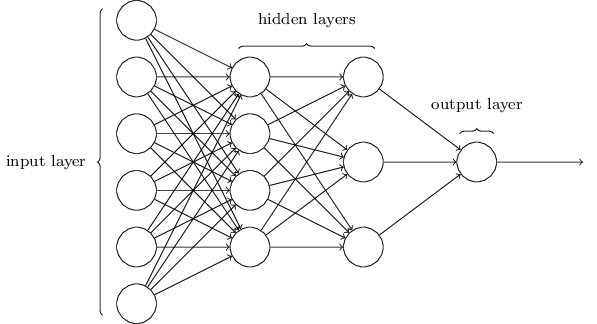
\includegraphics[width=0.7\textwidth]{nn_layers}
    \caption{Neural network's structure and layers (from \textit{Neural Networks and Deep Learning} free online book)}
    \label{fig:nn_layers}
\end{figure}

The most classic form of neural networks is the \textit{feed-forward neural network} \acs{fcnn}, also called dense neural network. A \acs{fcnn} consists of a sequence of fully-connected layers \cite{OReilly:TFforDL}. Each layer represents a function (linear and non-linear transformations) from $\mathbb{R}^F$ to $\mathbb{R}^{F_m}$. This means that, for each input instance having $F$ features, the corresponding output will have dimensionality $F_m$, where $F_m$ is the number of neurons in the network's output layer (the $m$-th layer). Even for the hidden layers, the output dimension depends on the number of neurons present in the layer.

The network is called \textit{fully-connected} because the output of each neuron in one layer is sent as input of each neuron in the next layer, so there is a direct connection between all the neurons belonging to subsequent layers. Figure \ref{fig:nn_dense} shows and example of dense neural network, making visible the full interconnection between subsequent layers.
\begin{figure}[htbp]
    \centering
    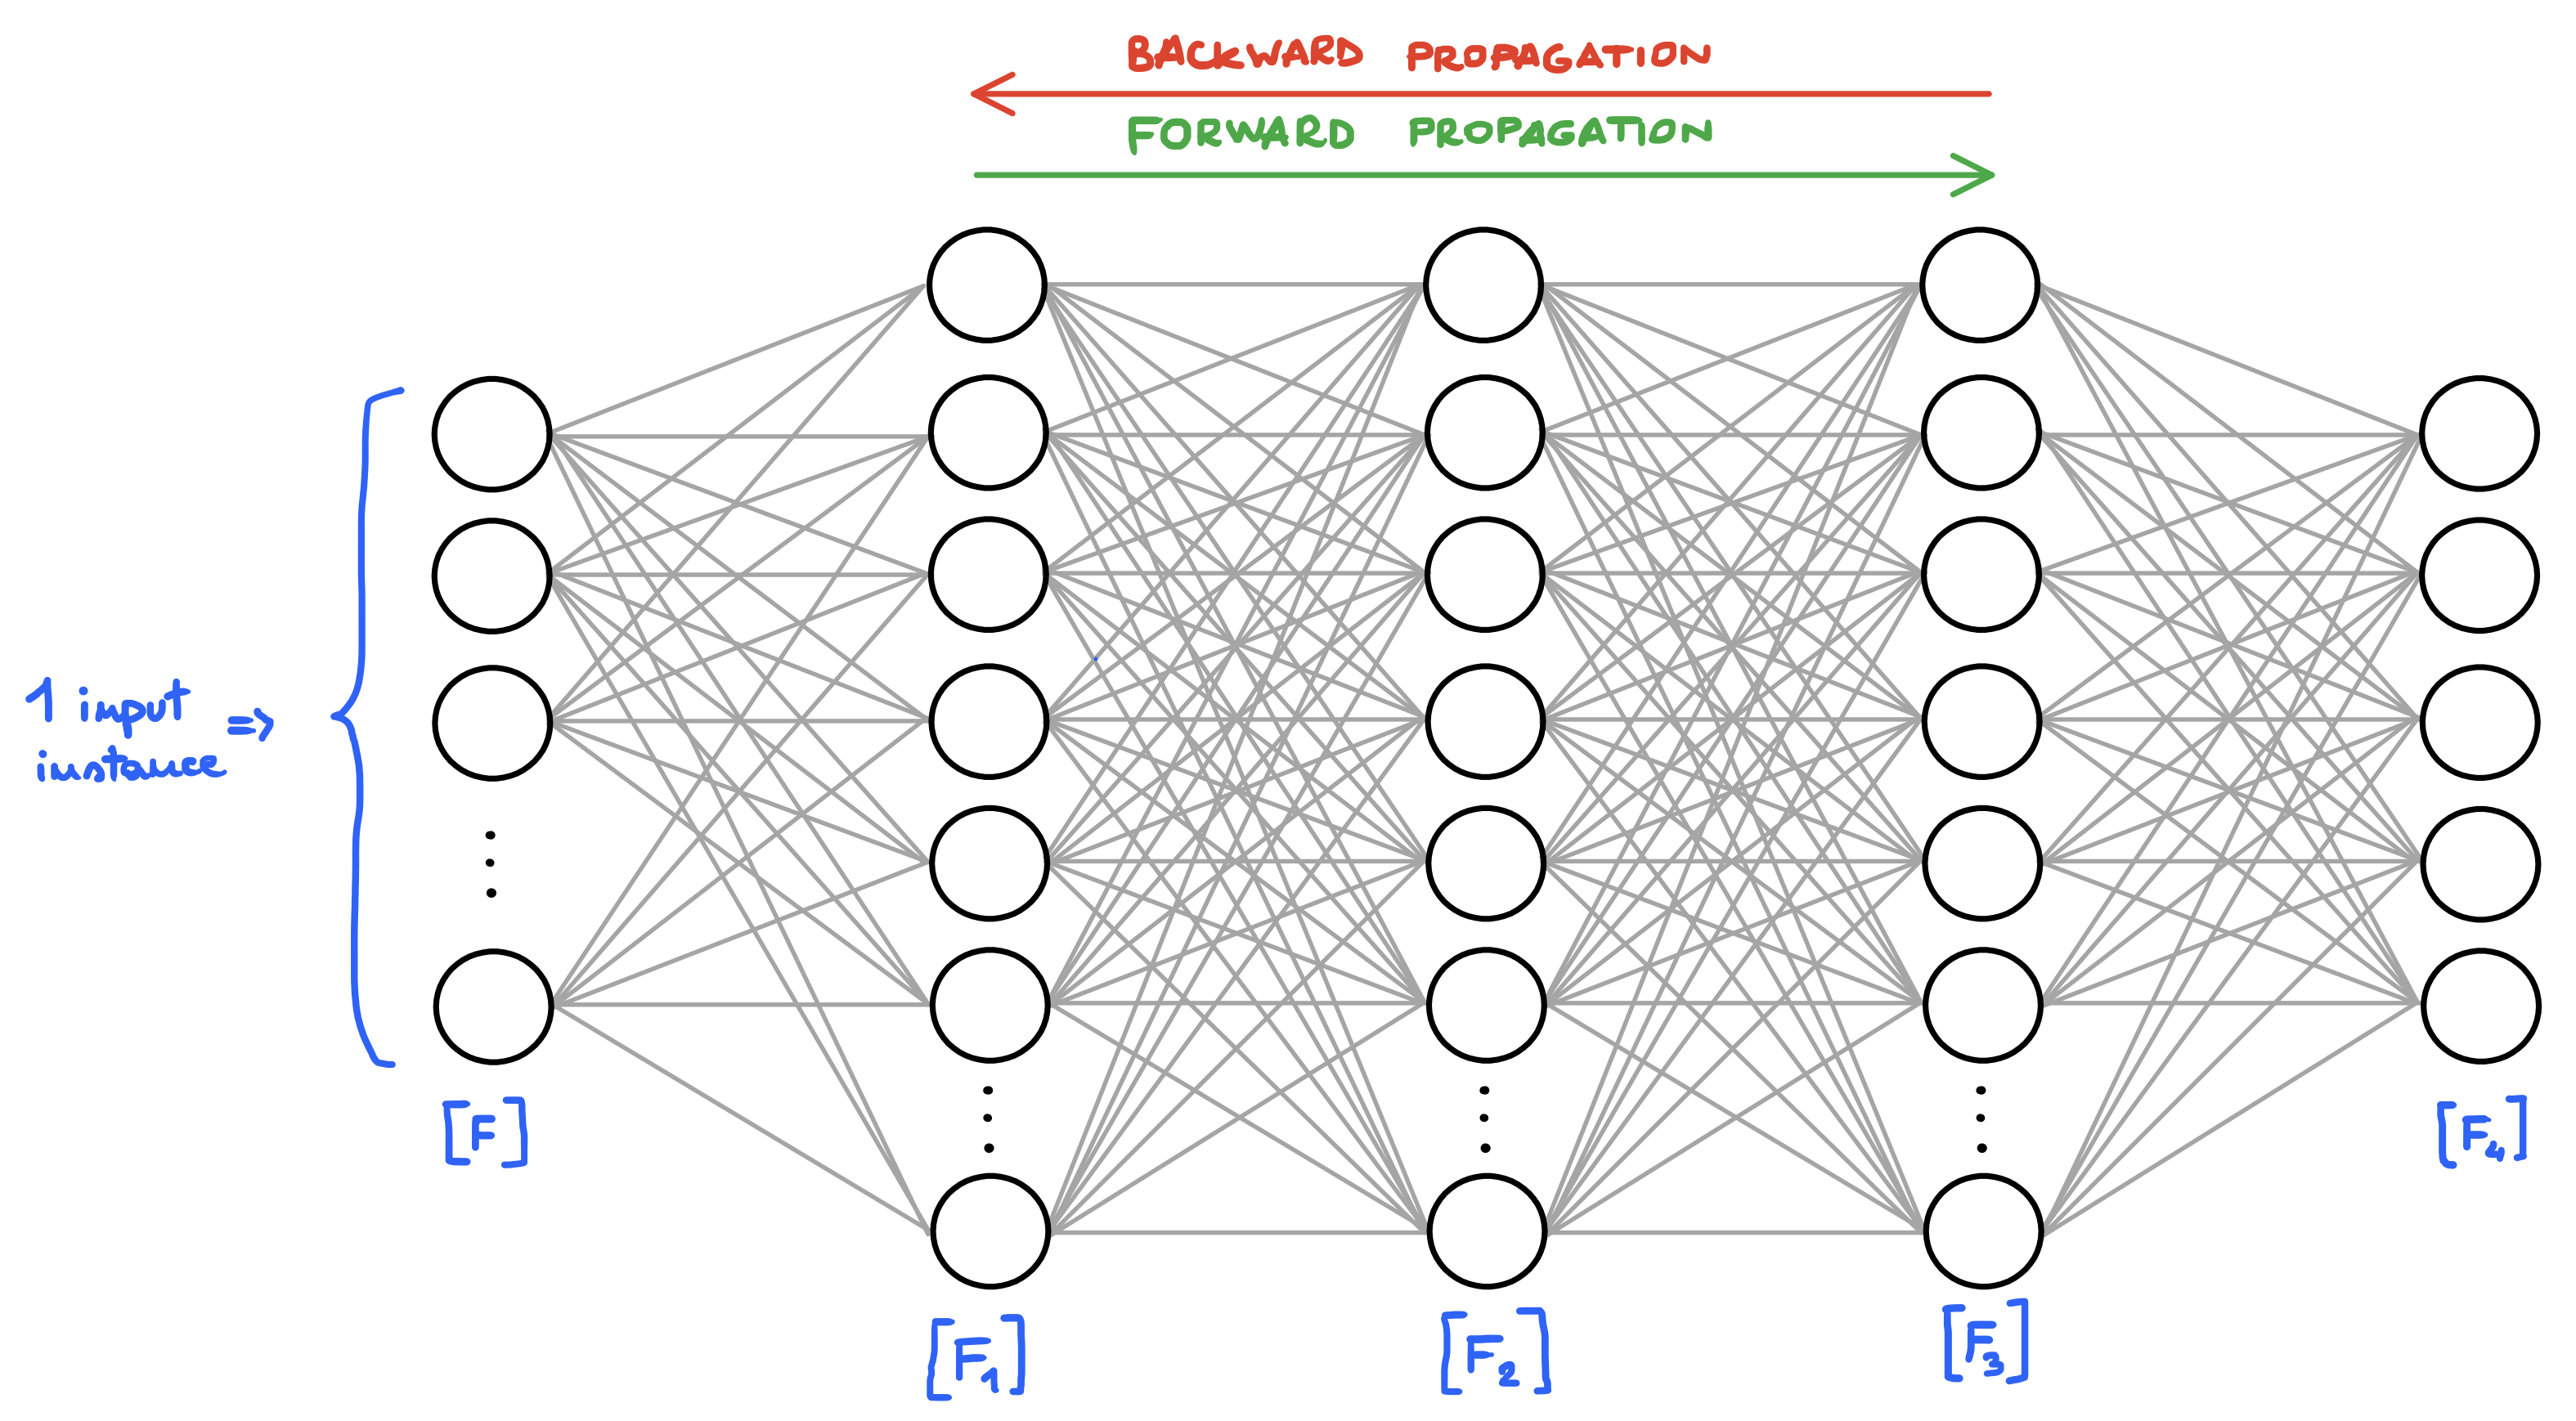
\includegraphics[width=0.9\textwidth]{nn_dense}
    \caption{Example of dense neural network}
    \label{fig:nn_dense}
\end{figure}

Each neuron processes the input data by computing the following transformation:
\begin{align}
    \mathbf{x}_{i}^{l}=\sigma\left(\sum_{j} \mathbf{w}_{ij}^{l} \mathbf{x}_{j}^{l-1} + \mathbf{b}_{i}^{l}\right)
\end{align}
where the subscript represent the $i^{th}$ or $j^{th}$ neuron of the layer in the superscript, which is the $l^{th}$ or $(l-1)^{th}$ layer, $\mathbf{x}$ represents the input features, $\mathbf{w}$ represents the correspondent weights, $\mathbf{b}$ represents the bias term, usually equal to 1, and $\sigma$ represents the activation function. The weighted sum plus the bias term form the linear part of the transformation, followed by the non-linear part, which is the application of the activation function. The bias term helps the network approximating the objective function; while the activation function, as already mentioned, introduces the non-linearity properties by mapping the data to the desired output. Figure \ref{fig:nn_neuron} illustrates the functioning of a single neuron.
\begin{figure}[htbp]
    \centering
    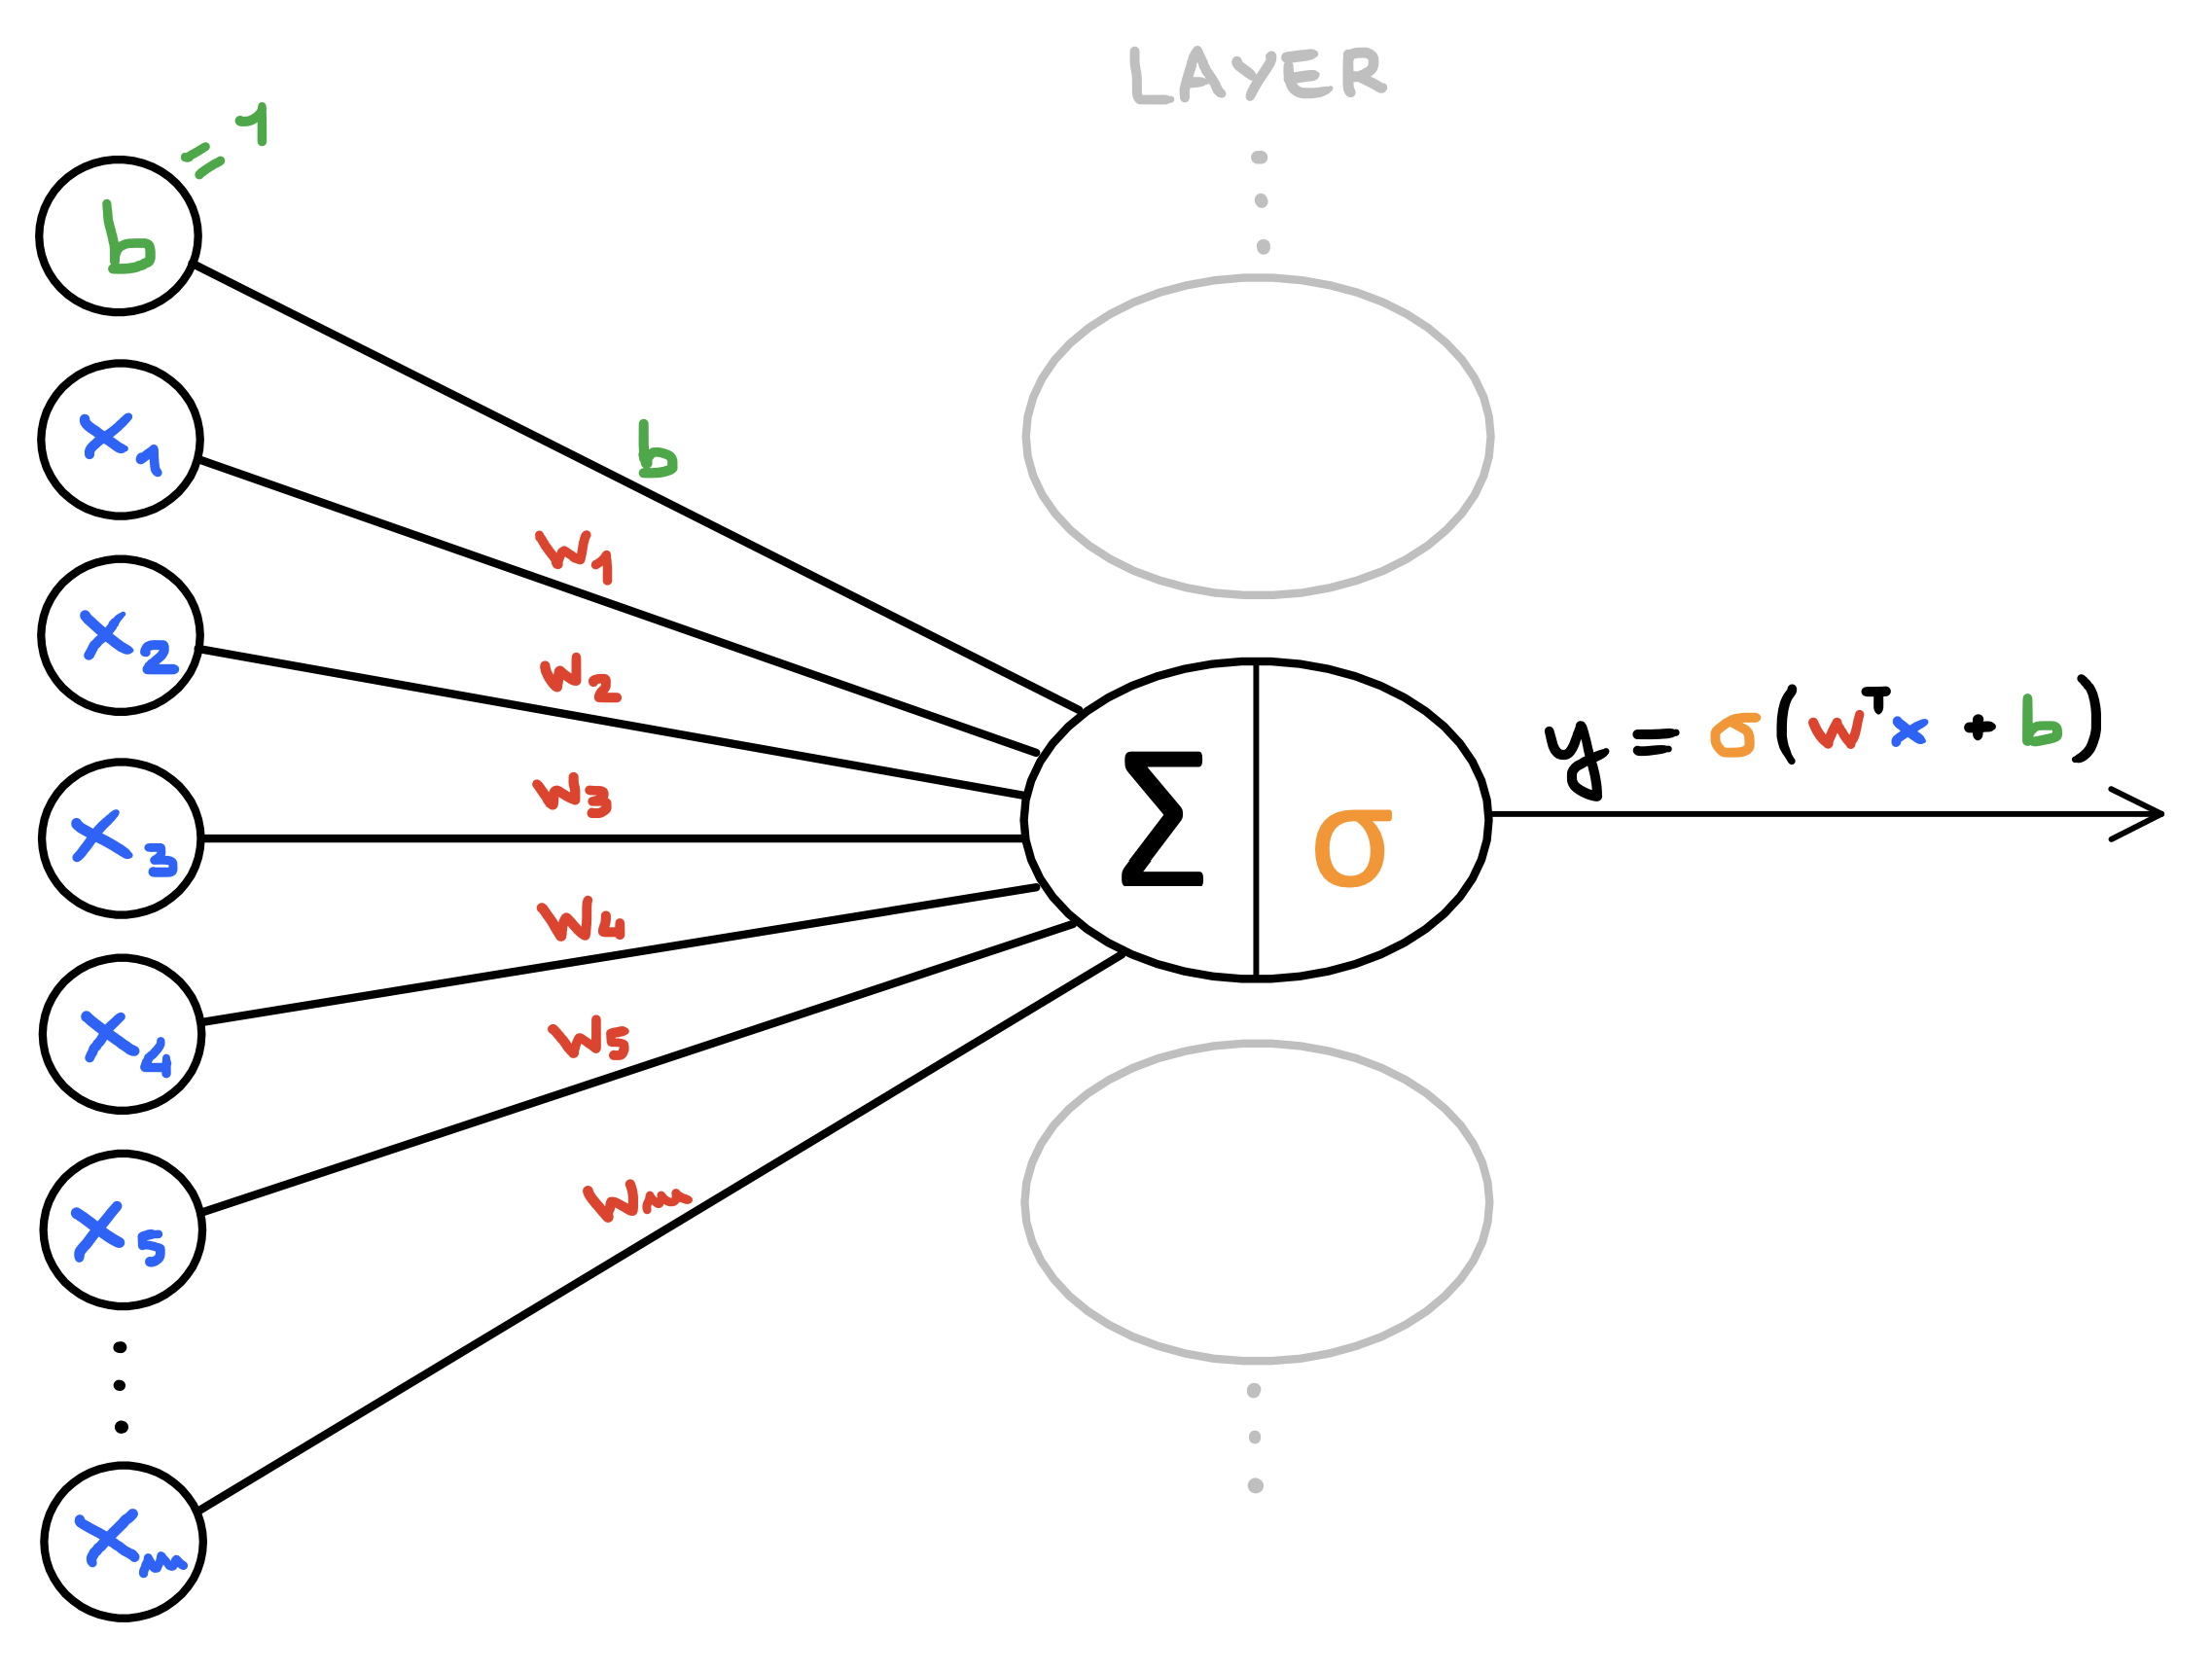
\includegraphics[width=0.6\textwidth]{nn_neuron}
    \caption{Illustrated description of the functioning of a single neuron}
    \label{fig:nn_neuron}
\end{figure}

Each neuron in a layer performs this operation and the outputs of all the neurons of that layer will be the inputs for the next layer. Formally, the inputs and outputs of layers of a neural network can be described by the equations:
\begin{align}
    &h^{\textit{out}}_{0} = \mathbf{X}\qquad\qquad\qquad \text{(input layer)}\\
    &h^{\textit{in}}_{i} = h^{\textit{out}}_{i-1} \times \mathbf{W}_i + \mathbf{B}_i\\
    &h^{\textit{out}}_{i} = \phi_i (h^{\textit{in}}_{i})
\end{align}
where $\mathbf{X}$ is the features matrix of input data, $\mathbf{W}_i$ is the weights matrix of layer $i$, $\mathbf{B}_i$ is the bias vector of layer $i$, $\phi_i$ is the activation function used by neurons of layer $i$, and the operator $\times$ represents matrix multiplication.

When used for classification tasks, the output layer of a \acs{fcnn} has a number of neurons that is equal to the number of classes of the data. In this way, each output of the network (computed through softmax or sigmoid activation function) corresponds to the estimated probability that the input instance belongs to the corresponding class. The instance is then assigned to the class which obtained higher probability.

\subsection{Neural network's training process}
\paragraph{} The training process of neural networks takes places through two steps: the forward and backward propagations. For each training input instance, the model computes the output of every neuron in each consecutive layer until it reaches the final predictions from the output layer (\textit{forward pass)}. After that, it compares its prediction with the actual targets and measures the output error. The error is then propagated through each layer in reverse in order to compute the error contribution (error gradient) from each neuron's connection, until it reaches the input layer (\textit{backward pass}). The error is then used by the optimizer to update the connections weights and allow the model to learn. The neural networks in which the activation flows only in one direction are included in the category of feed-forward neural networks.

The \textit{backpropagation} represents the core of the learning process of a neural network, since it is the procedure to update the model's learnable parameters. After the generation of the predictions (forward pass), the gradient of the loss function with respect to the weights is computed; then the weights are updated in the opposite direction of the gradient. This operation is called \textit{Gradient Descent}. The "magnitude" of the update is given by the \textit{learning rate}, which can be decisive in the search for the loss function's global minimum.


\subsection{Optimizers}
\paragraph{} An optimization algorithm determines the way in which the model's parameters (\textit{weights}) are updated during the training process. The aim of an optimizer is to minimize an objective function that is dependent on the model's weights, which is the cost function. Since the cost function is computed using the model's predictions and the latter are determined by the weights and input features, the weights have a crucial role in minimizing the cost function. Since the weights values are determined by the Gradient Descent, the role of an optimizer is to optimize the Gradient Descent process, in order to make it more efficient and effective. In this project, the optimizer that has been used for all the models is the \acf{adam} optimizer.

\paragraph{\acs{adam} optimizer} \acs{adam} is one of the most popular and used optimizers in deep learning, that usually has good performances. It is based on two intuitions: adaptive learning rate (inspired by RMSProp optimizer) and momentum optimization \cite{arXiv:adam} \cite{arXiv:optimizers}. An adaptive learning rate method computes individual learning rates for different model's learnable parameters; while a momentum method helps accelerating the Gradient Descent process by adding a fraction of the update vector of the past time step to the current update vector. This optimizer stores two moments: the first moment $m_t$ (the mean), which is estimated as the exponentially decaying average of past gradients, and the second moment $v_t$ (the uncentered variance), which is estimated as the exponentially decaying average of past squared gradients. The two moments are computed respectively as follows:
\begin{align}
    m_{t} &=\beta_{1} m_{t-1}+\left(1-\beta_{1}\right) g_{t} \\
    v_{t} &=\beta_{2} v_{t-1}+\left(1-\beta_{2}\right) g_{t}^{2}
\end{align}
where $g_{t}$ is the gradient on current mini-batch and $\beta_1$, $\beta_2$ are optimizer's decay rates, usually set close to 1. Since $m_t$ and $v_t$ are initialized as zero-vectors, they are biased towards zero, therefore they need to be corrected:
\begin{align}
    \hat{m}_{t} =\frac{m_{t}}{1-\beta_{1}^{t}} \qquad\qquad\qquad
    \hat{v}_{t} =\frac{v_{t}}{1-\beta_{2}^{t}}
\end{align}
The first moment $m_t$ is used as momentum optimization parameter, while the second moment $v_t$ is used to adapt the learning rate to each different weight. The resulting \acs{adam} update rule for model's weights is the formula:
\begin{align}
    \theta_{t+1}=\theta_{t}-\frac{\eta}{\sqrt{\hat{v}_{t}}+\epsilon} \hat{m}_{t}
\end{align}
where $\theta$ is the model weight and $\eta$ is the learning rate ($\epsilon$ is just a smoothing term usually initialized to a tiny number).


\subsection{Activation functions}
An activation function is a non-linear mapping between the input and the output. Activation functions are essential in neural networks layers, since they introduce the non-linearity properties to the model: without activation functions, the neural network would be a simple linear transformation and it wouldn't be able to learn from complex data.

Some activation functions are more suited to hidden layers, while others are perfect to compute the final output of the model. In this project, we used the sigmoid function as activation function for the last layer of our models in order to classify data, as previously explained in Section \ref{sec: classification}. For the hidden layers, we used both \acf{relu} and \acf{tanh} activation functions.

\paragraph{ReLU} \acs{relu} is a very popular and extremely fast and effective activation function for hidden layers. Its principle is very simple: it keeps only positive values, while setting to 0 all the negative ones.
\begin{align}
    \text{R}(x) = max(0, x)
\end{align}
The \acs{relu} function is illustrated in Figure \ref{fig:relu}. The \acs{relu} activation function is very effective for very deep networks, since it helps avoiding the vanishing gradient problem. This problem arises when the gradient of the loss function, used to update the model's weights, assumes too small values during the backpropagation across the layers and the network is not able to learn anymore. \acs{relu}, thanks to the sparsity of its outputs, helps avoiding this problem.

\paragraph{Tanh} \acs{tanh} is similar to sigmoid, but it ranges from $-1$ to $1$. It maps negative input as strongly negative, positive ones as strongly positive and zero inputs near zero. Its formula is:
\begin{align}
    \tanh{(x)} = \frac{e^{2x} - 1}{e^{2x} + 1}
\end{align}
The \acs{tanh} function is illustrated in Figure \ref{fig:tanh}.
\begin{figure}[htbp]
    \centering
    \begin{subfigure}[t]{0.5\textwidth}
		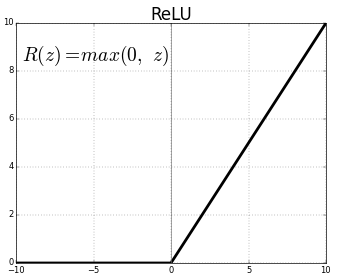
\includegraphics[width=0.9\textwidth]{relu}
        \caption{ReLU activation function (from \textit{Medium})}
        \label{fig:relu}
	\end{subfigure}%
	~
	\begin{subfigure}[t]{0.5\textwidth}
		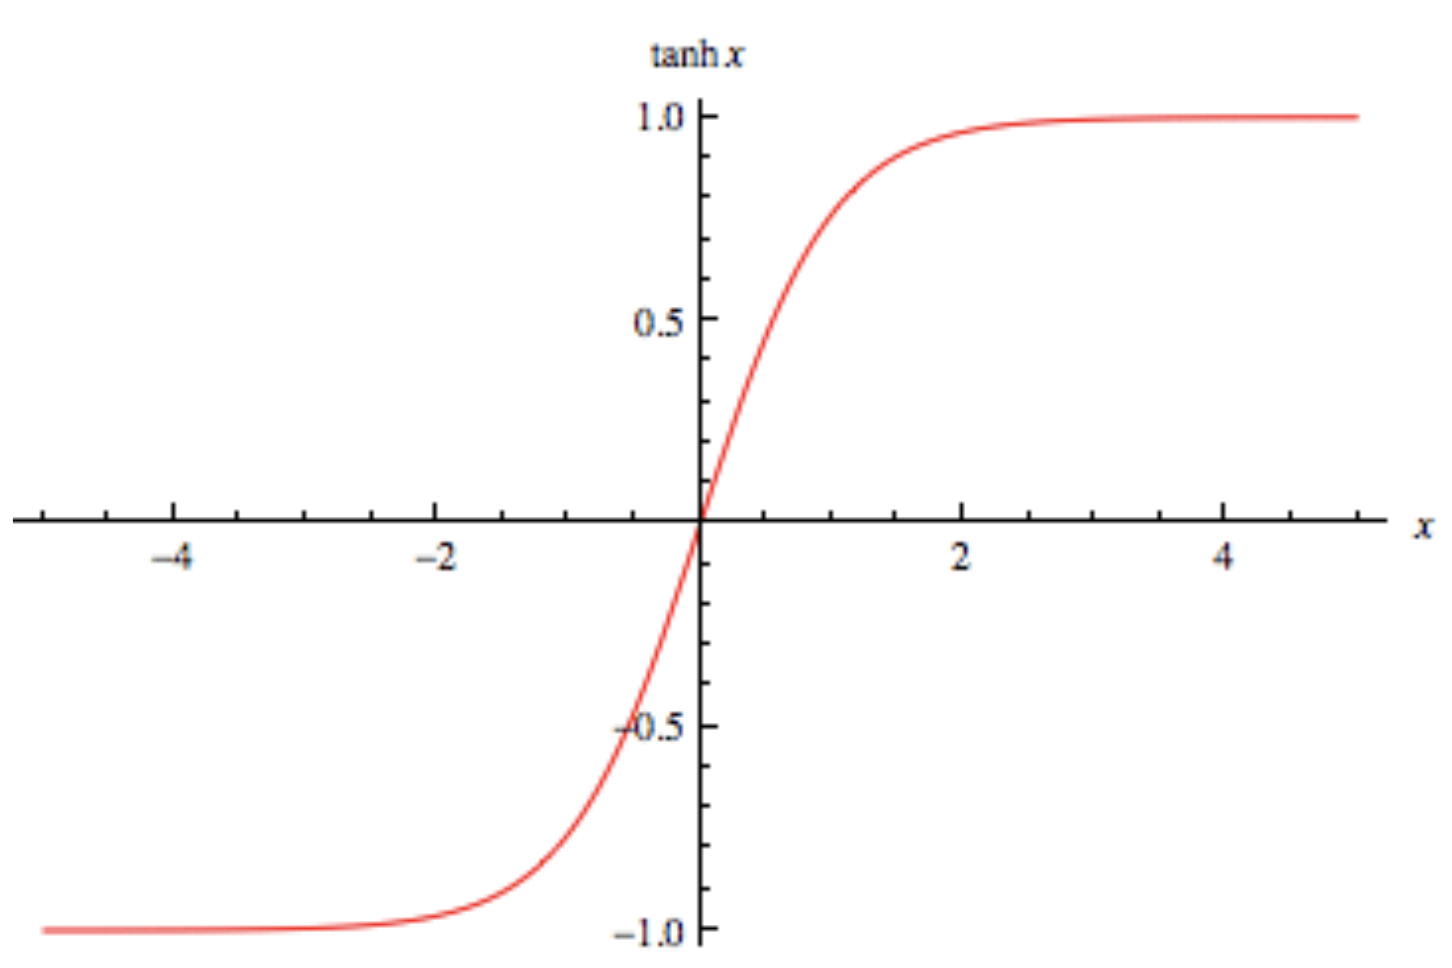
\includegraphics[width=1\textwidth]{tanh}
        \caption{Tanh activation function (from \textit{Wolfram MathWorld})}
        \label{fig:tanh}
	\end{subfigure}
	\caption{Activation functions}
\end{figure}


\subsection{Regularization}
\paragraph{} Regularization techniques are very useful in deep learning in order to avoid overfitting. Deep neural networks generally have a huge amount of parameters, which represent their power to learn from complex datasets; this flexibility, however, sometimes leads to the overfitting of the training set, preventing the model from making good predictions on any other dataset \cite{OReilly:handsonML}. To solve this problem, there exist several regularization methods, which in some way limit the amount of freedom of the model by encouraging the optimization process to find simpler solutions.

The regularization techniques used in this project are the $\ell_{2}$ regularization and dropout.

\paragraph{$\mathbf{\ell_2}$ regularization} The $\ell_2$ regularization, also called Ridge Regression or Tikhonov regularization, constrains the model's flexibility by adding a regularization term to the cost function. In this way, while trying to fit the data, the model is forced to keep the weights as small as possible. The regularization term added to the loss function is the 2-norm (Euclidean distance) squared, controlled by the parameter $\lambda$, which handles the amount of regularization of the model. This is expressed by the equation:
\begin{align}
    &\textit{regularization term } = \lambda \|\theta\|_{2}^{2} = 
    \lambda \sum_{i=1}^{m} \theta_{i}^{2}\\
    &\textit{error } = (\textit{loss function}) + \lambda \sum_{i=1}^{m} \theta_{i}^{2}
\end{align}
where $\|\cdot\|_{2}$ represents the 2-norm and $m$ is the length of the weights vector $\theta$ of the model. If $\lambda = 0$, then there is no regularization, since the regularization term added to the loss function is zero. If $\lambda$ is too large, then the weights take a value very close to zero and the model underfits the data, not being able to learn from it.

\paragraph{Dropout} Dropout is probably the most popular regularization technique in deep learning. The principle is very simple: during the training process, some layer's neurons are "dropped out", which means they are set to zero and completely ignored. The neurons to shut down are selected from each layer based on a probability $p$. This means that, at each training step, each neuron has a probability $p$ of being shut down for that training step. The probability $p$ represents the dropout rate, that is the fraction of nodes to ignore.
\begin{figure}[htbp]
    \centering
    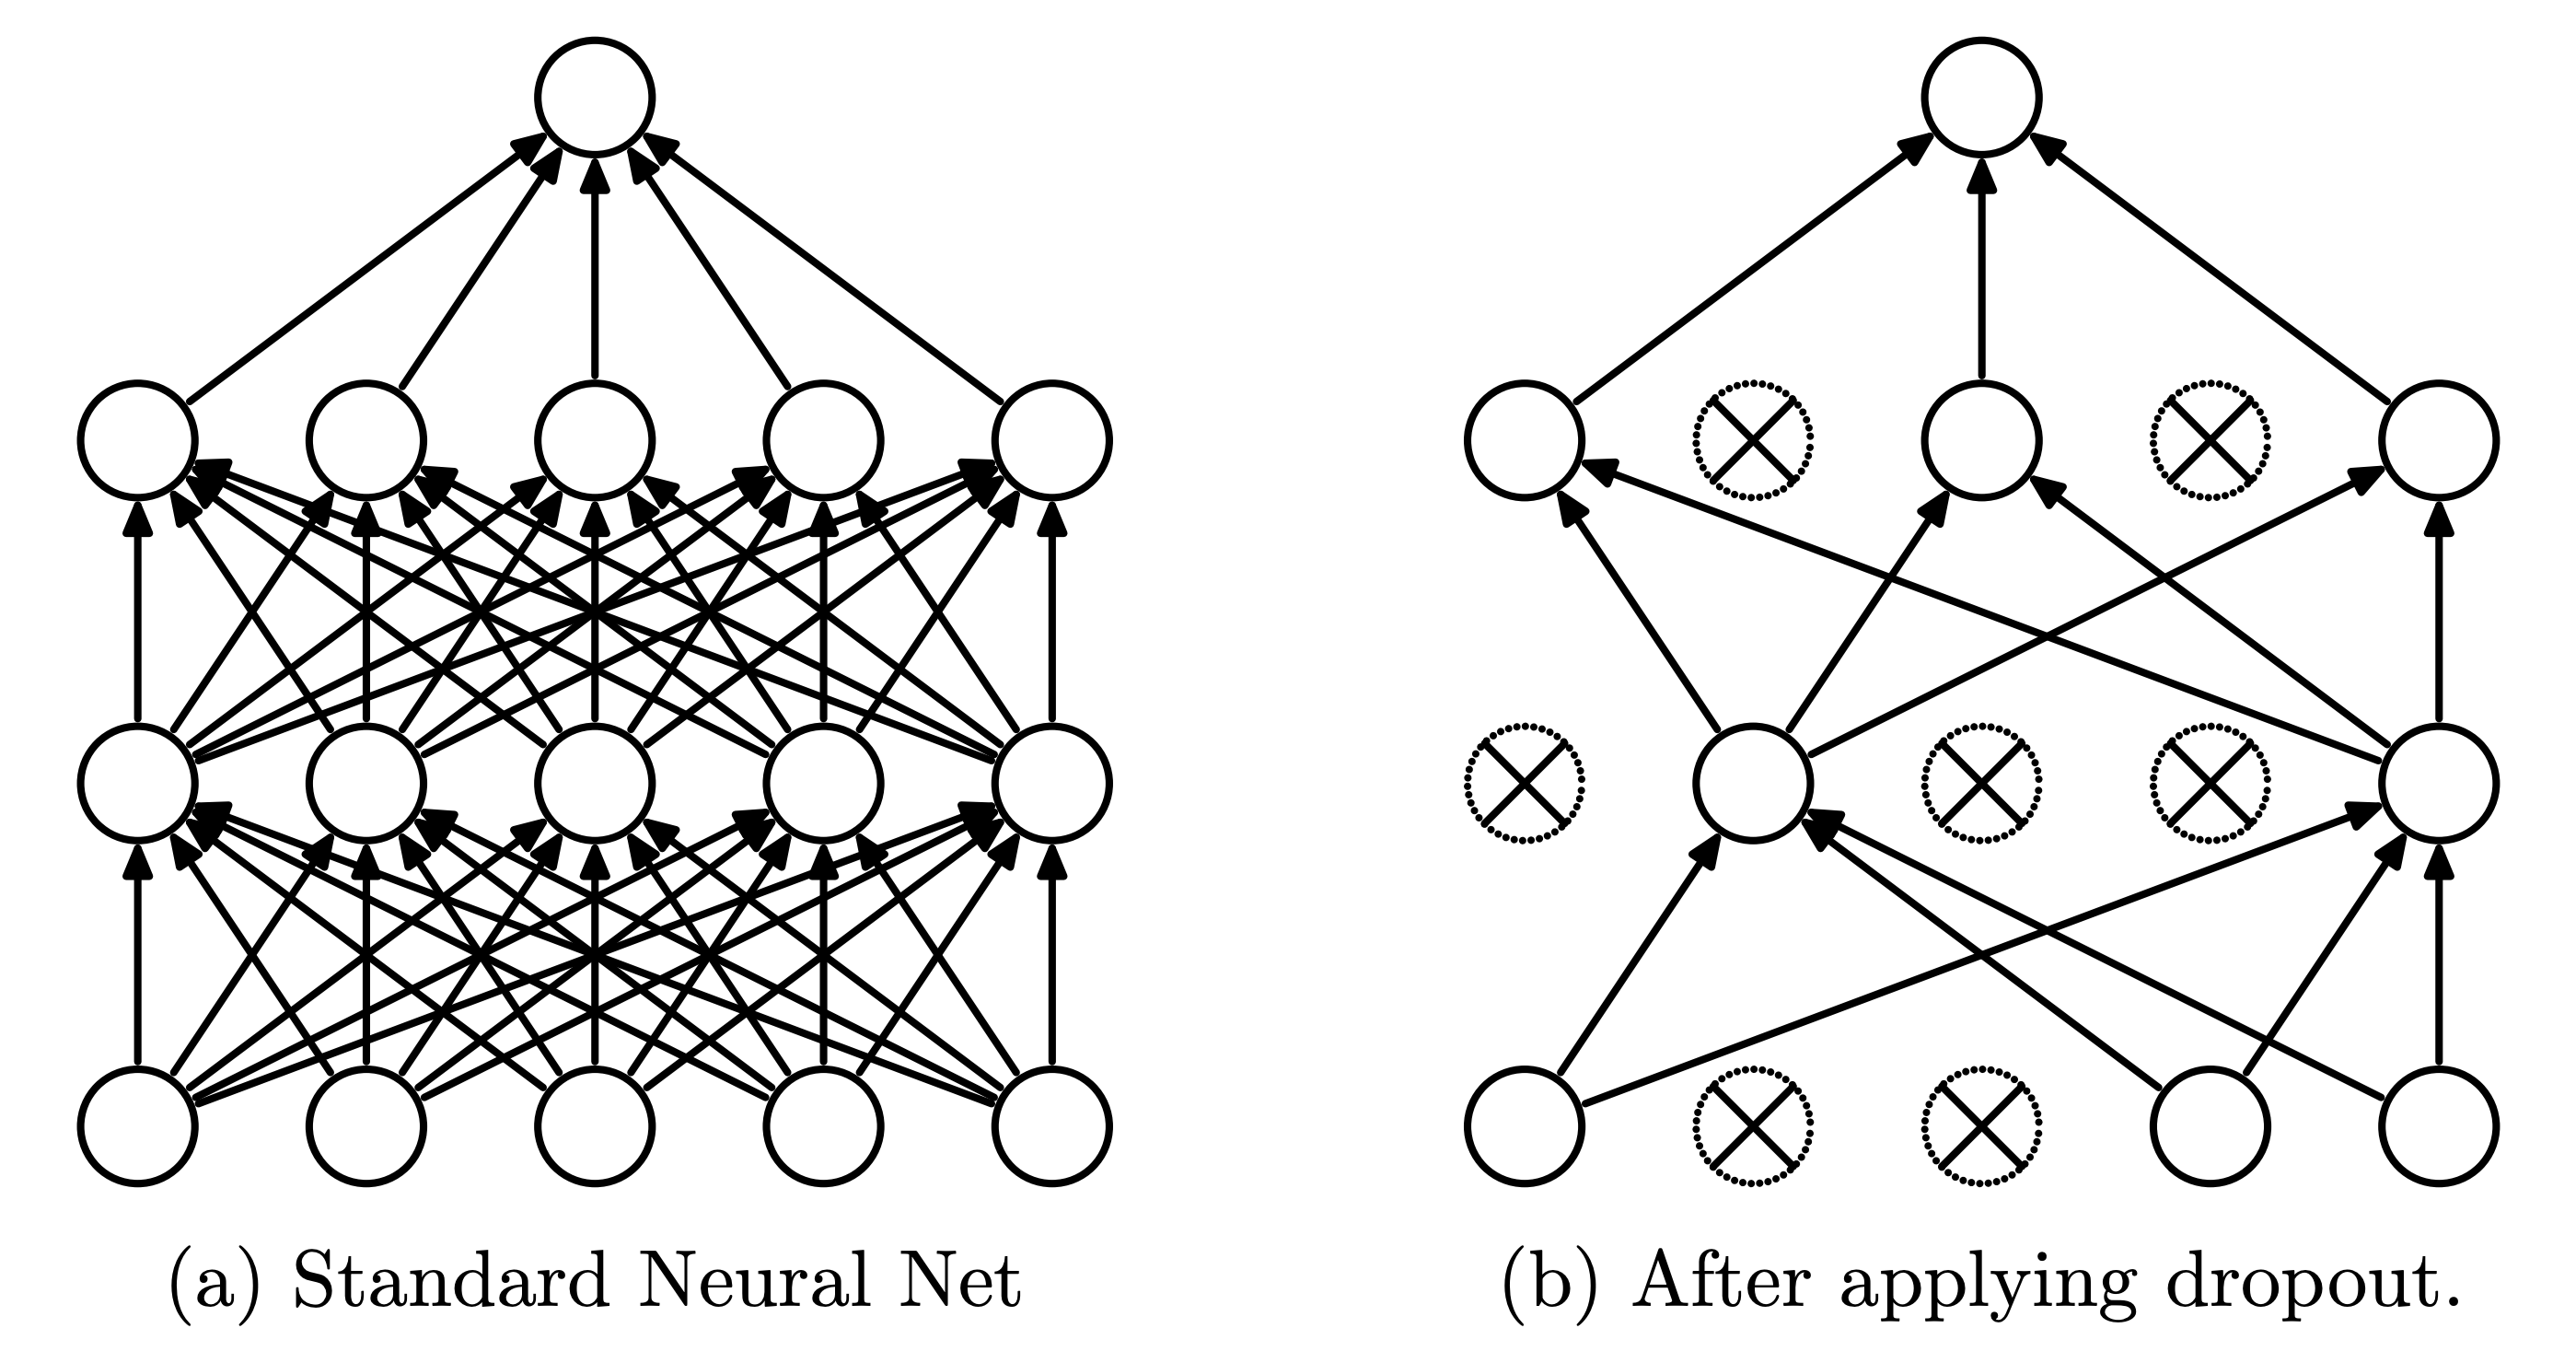
\includegraphics[width=0.7\textwidth]{dropout}
    \caption{Illustrated example of dropout (from \textit{Srivastava, Nitish, et al. ”Dropout: a simple way to prevent neural networks from overfitting”, JMLR 2014})}
    \label{fig:dropout}
\end{figure}

Figure \ref{fig:dropout} shows and example of dropout applied to a simple dense neural network. The idea behind dropout is that the network cannot rely on the features of each individual neuron, because if an essential neuron is shut down, then the network is not able to perform well. By ignoring some percentage of different neurons at each training step, the model is forced to learn more robust features, that work well together with the features of other groups of neurons. This approach prevents co-adaption, which is a situation that arises when some neurons are highly dependant on others. Dropout forces each single neuron to learn informative features, different from the ones learned by other neurons. In this way, a neuron is not dependant on the features of few individual neurons, leading to a better generalization.


\subsection{Convolutional neural network}
\paragraph{} Convolutional neural networks (\acsp{cnn}) are feed-forward networks that work very well especially for image recognition and complex visual tasks in general \cite{OReilly:handsonML}. A typical \acs{cnn} architecture consists of different building blocks: the convolutional layers, which identify low-level features in the image and learn to assemble them into higher-level features; the pooling layers, which subsample the image in order to reduce its dimensionality; finally, the dense network, which is at the end of the architecture and that uses the extracted features to make a prediction (see Figure \ref{fig:nn_conv}). Let's look at the functioning of convolutional and pooling layers.
\begin{figure}[htbp]
    \centering
    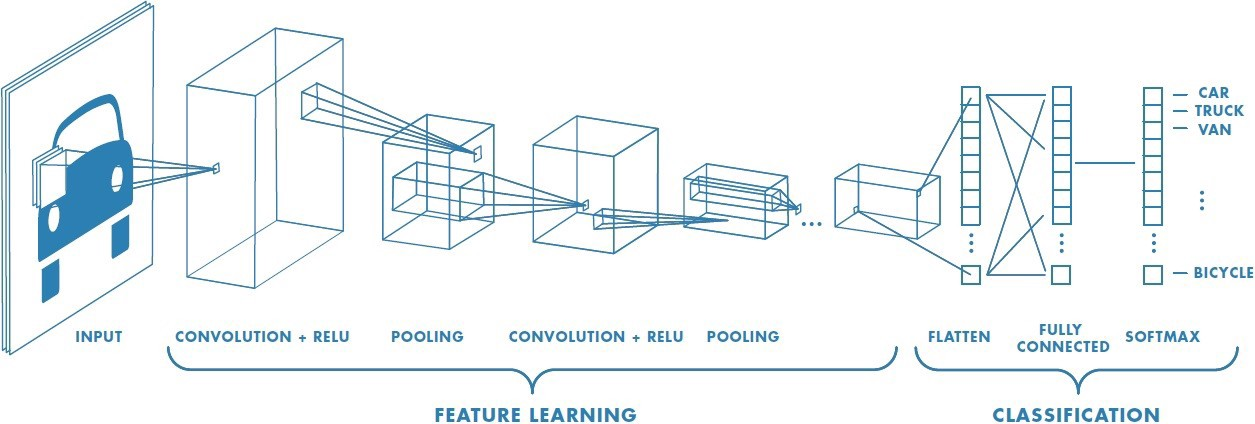
\includegraphics[width=1\textwidth]{nn_conv}
    \caption{Typical architecture of a convolutional neural network (from \textit{Medium - Towards Data Science})}
    \label{fig:nn_conv}
\end{figure}

Convolutional layers are different from dense layers only for the fact that they are not fully-connected: in convolutional layers, neurons are not connected to all previous layer's neurons, but only to neurons in their receptive fields. If we represent one layer's neurons mapped in 2D as a matrix, we can say that each neuron in the current matrix $l$ looks at a limited region of the previous matrix $l-1$, so it is connected only to neurons located within that region, as shown in Figure \ref{fig:nn_conv_layer}. This architecture allows to focus on low-level features in the first layer, where neurons look at small regions of the input image, and to aggregate them in high-level features in the following layers, where neurons combine lower-level features form the previous layer.
\begin{figure}[htbp]
    \centering
    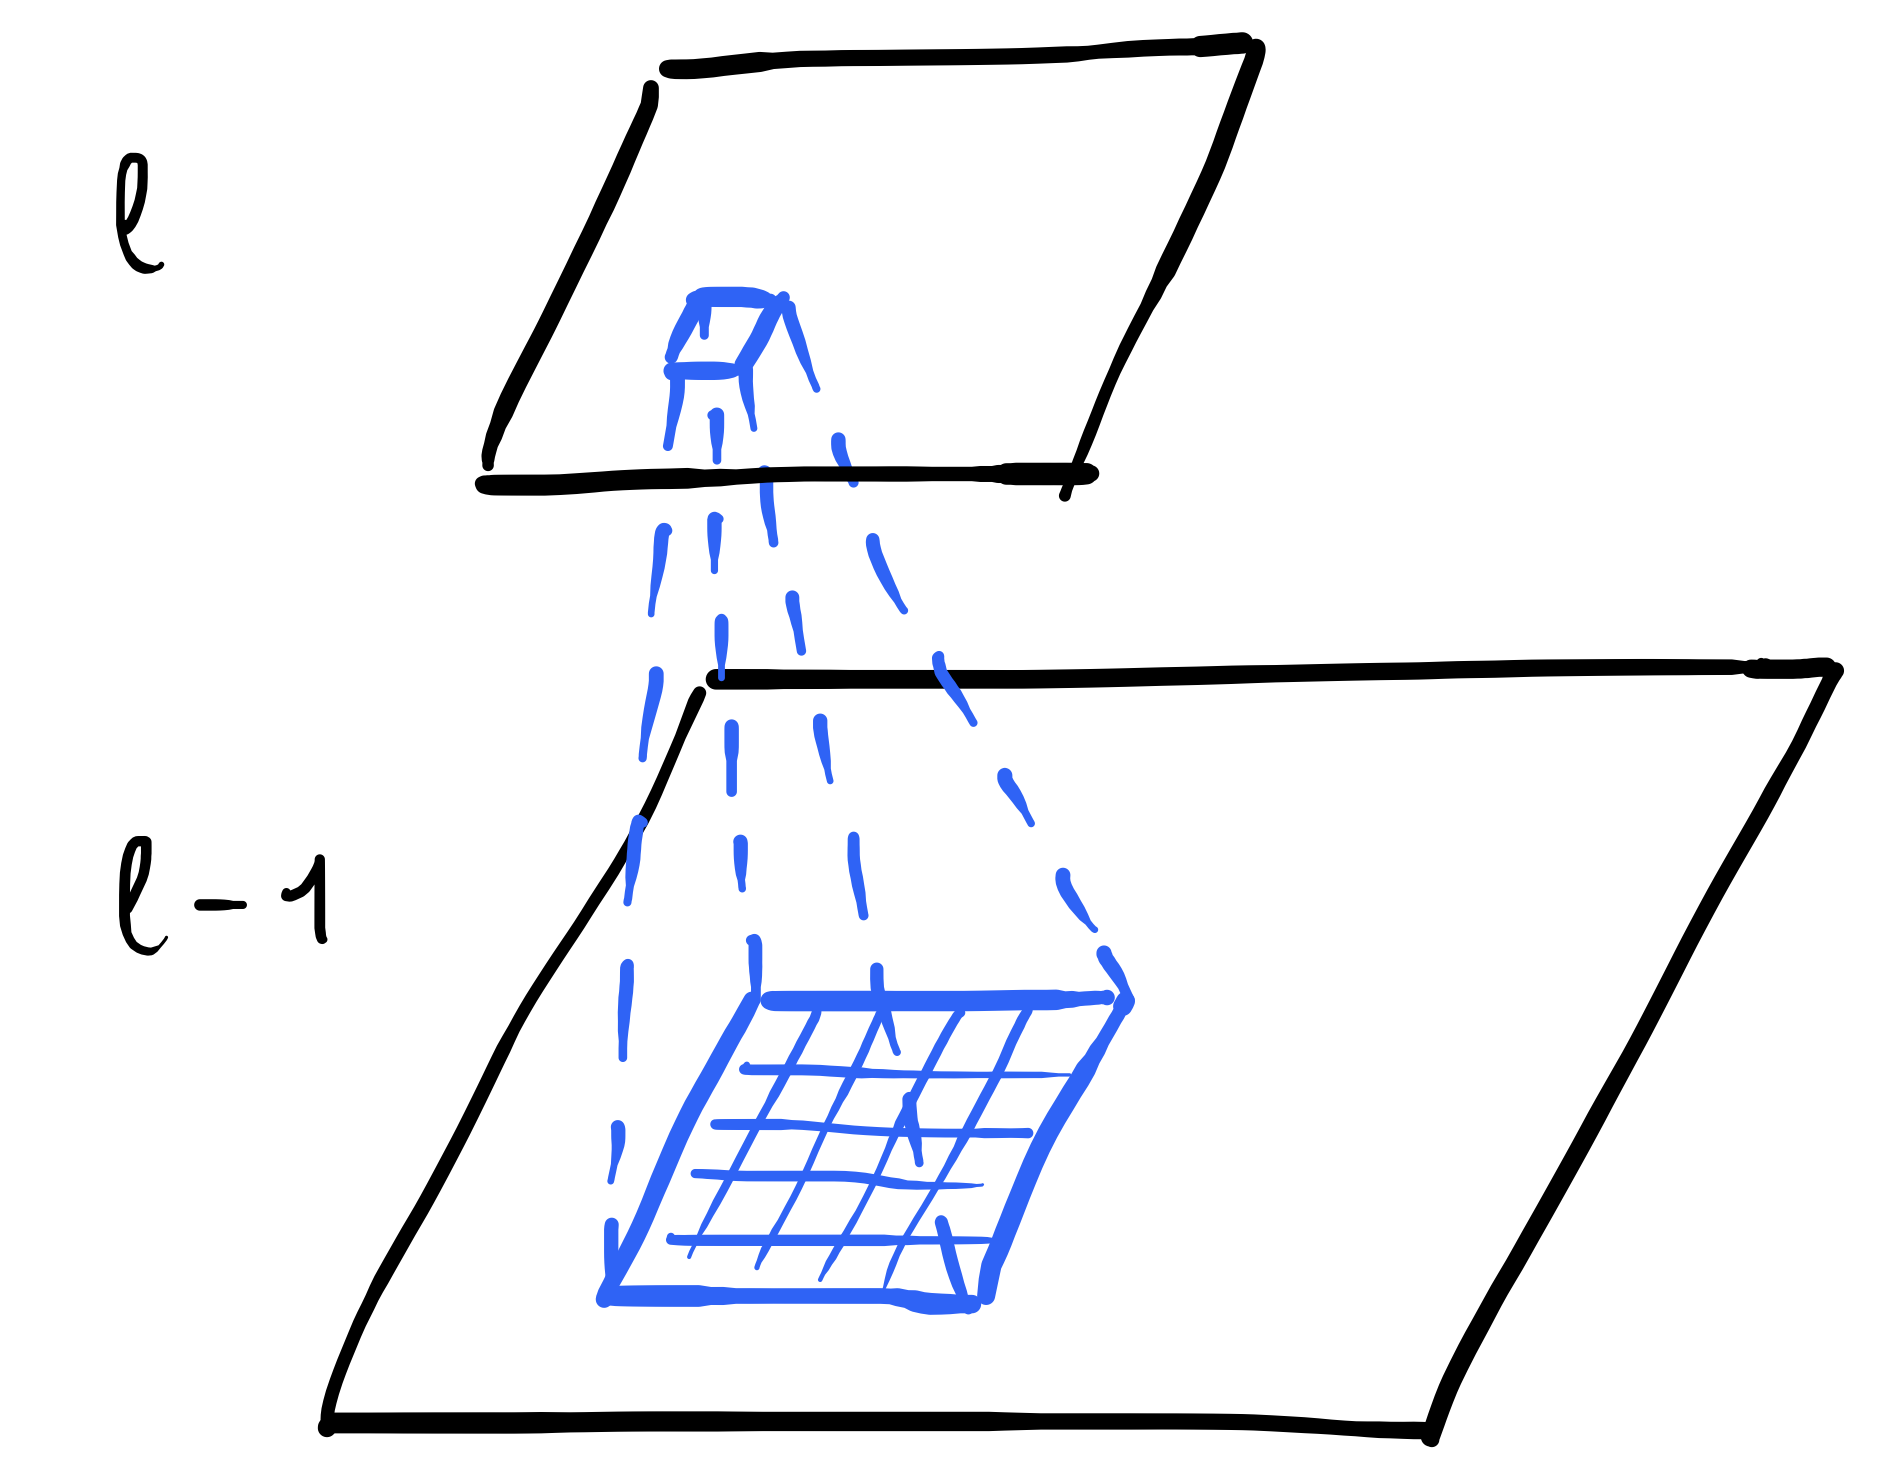
\includegraphics[width=0.35\textwidth]{nn_conv_layer}
    \caption{Relation between convolutional layer's neurons}
    \label{fig:nn_conv_layer}
\end{figure}

\begin{figure}[htbp]
    \centering
    \begin{subfigure}[t]{0.25\textwidth}
		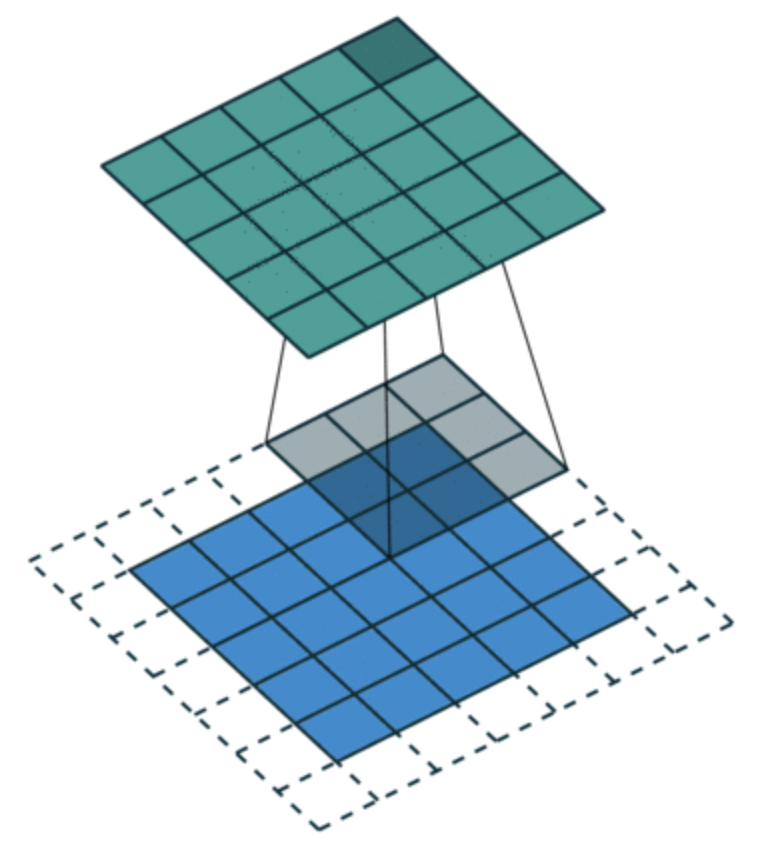
\includegraphics[width=1\textwidth]{nn_conv_padding}
        \caption{Zero padding}
        \label{fig:nn_conv_padding}
	\end{subfigure}
	~
	\begin{subfigure}[t]{0.8\textwidth}
		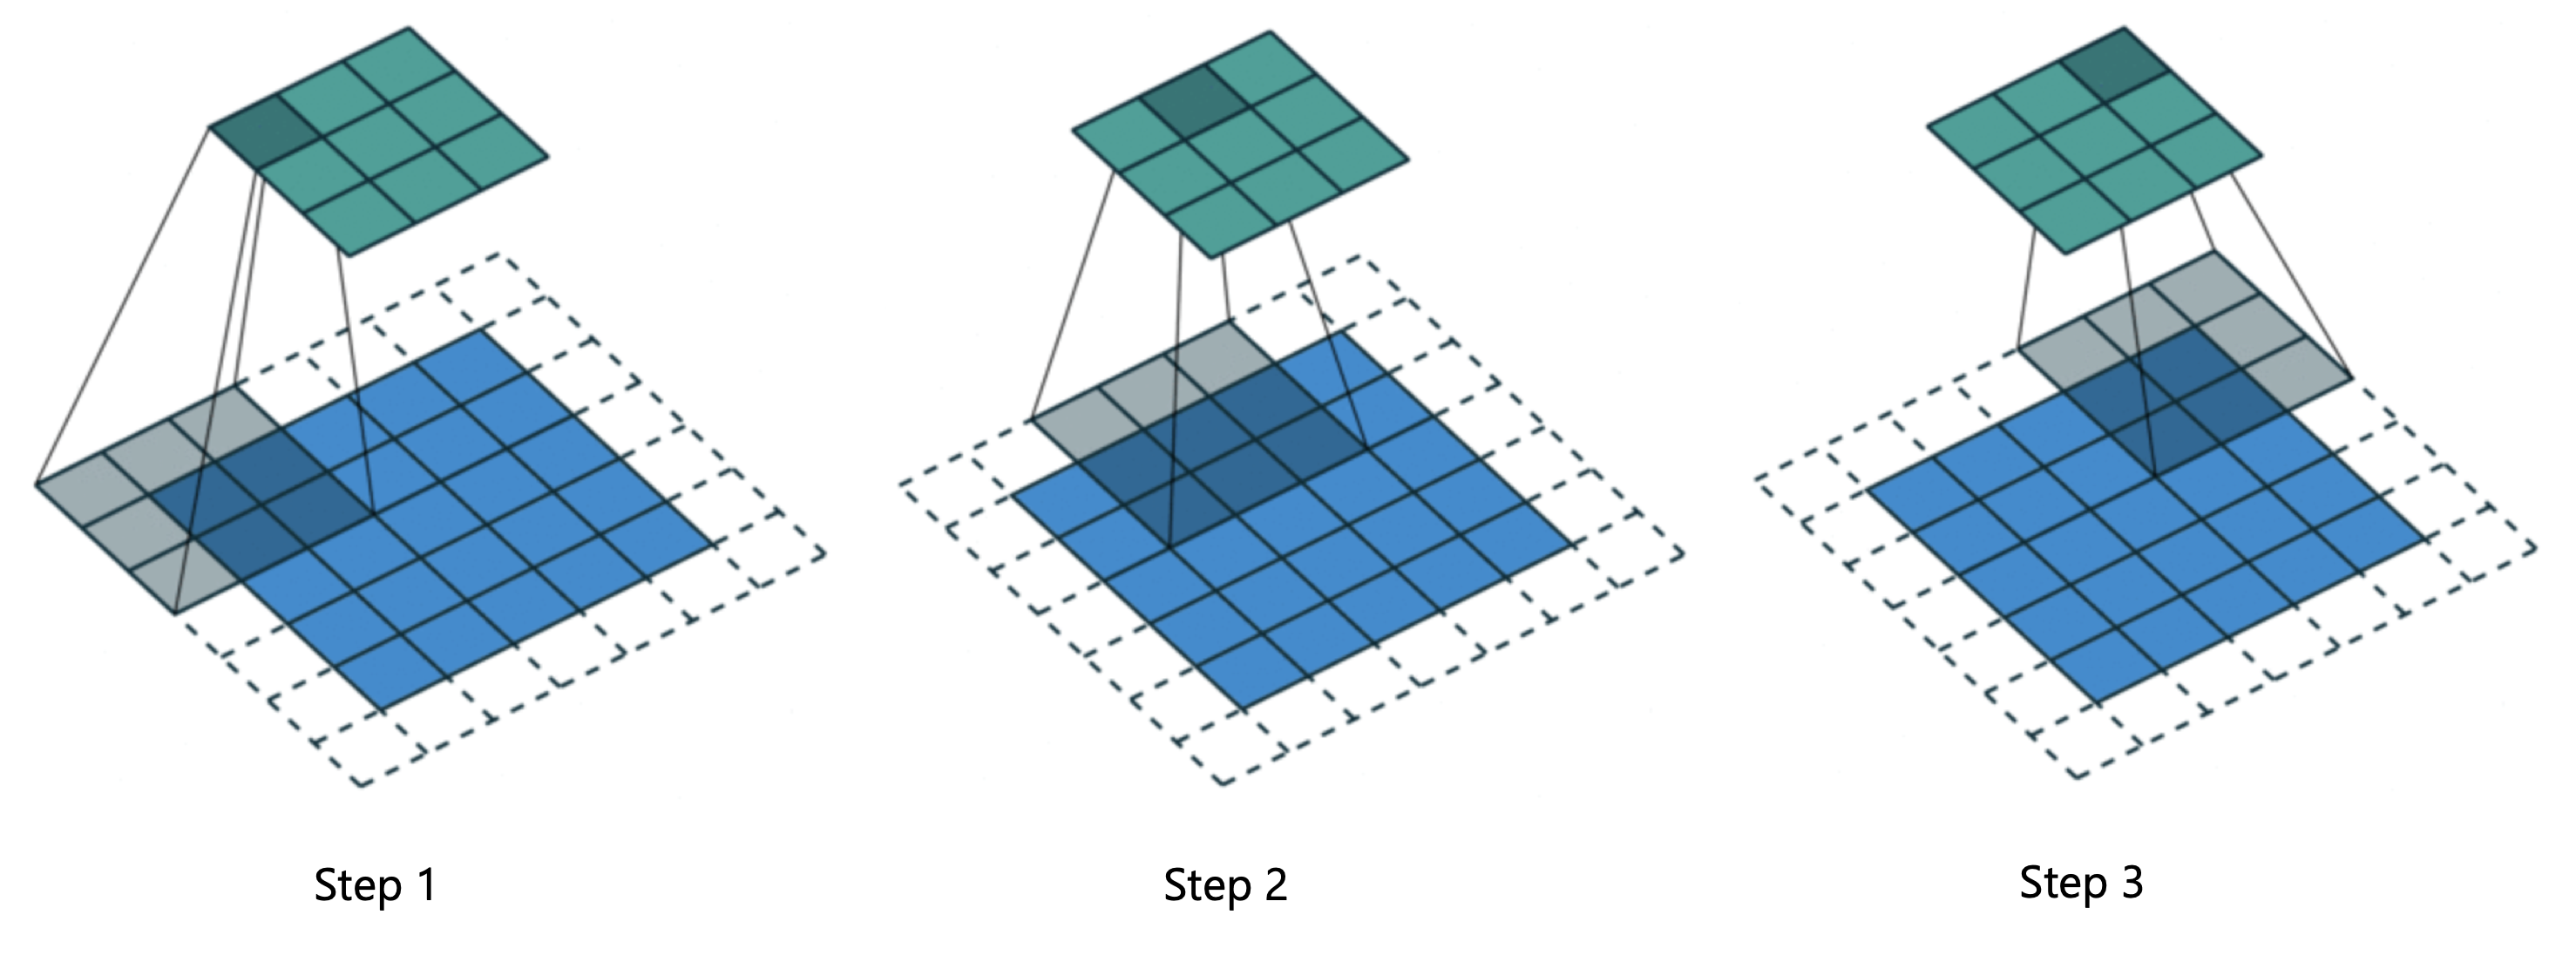
\includegraphics[width=1\textwidth]{nn_conv_stride}
        \caption{Sequence of receptive fields with stride equal to 2}
        \label{fig:nn_conv_stride}
    \end{subfigure}
    \caption{(from \textit{Medium - Towards Data Science})}
    \label{fig:padding_stride}
\end{figure}

In order for a layer to have the same dimensionality of the previous layer, zero padding can be applied by adding a zero-frame to the previous layer (Figure \ref{fig:nn_conv_padding}). In order for a layer to have a much smaller dimensionality with respect to the previous layer, we can use a higher stride, which is the distance between two subsequent receptive fields. By default, the stride is set to 1, so usually the difference between two receptive fields is is one row/column of neurons; by increasing the stride, a smaller number of receptive fields is taken into consideration, therefore the following layers is much smaller (Figure \ref{fig:nn_conv_stride}).

In a convolutional layer, neurons weights are represented by \textit{filters} (also called \textit{kernels}). A filter is a matrix of the same size of the receptive field and it contains the weights that are applied to the corresponding receptive field. The application of the same filter to all the receptive fields of an image produces a feature map, which identify and highlight the details of the image that are most similar to the filter. A convolutional layer is composed by several feature maps of equal size, that in practice corresponds to having multiple matrices of neuron stacked together generating a third dimension, which is the number of feature maps. In a convolutional layer, all neurons in the same feature map share the same weights and bias, so they all use the same filter, while from layer to layer the filter used is different. In this way, the convolutional layer applies different filters to the input image and each feature map can specialize on identifying a specific image feature. Figure \ref{fig:nn_conv_filter} shows a $3\times3$ filter applied over three feature maps (depth); for example, it could be the case of a color image composed of three color channels, which correspond to the three feature maps.
\begin{figure}[htbp]
    \centering
    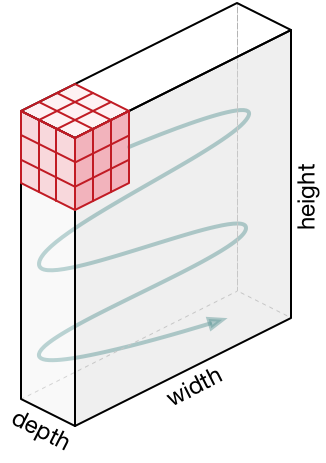
\includegraphics[width=0.3\textwidth]{nn_conv_filter}
    \caption{Movement of a $3\times3$ filter applied over three feature maps (from \textit{Medium - Towards Data Science})}
    \label{fig:nn_conv_filter}
\end{figure}

Convolutional layers are usually followed by pooling layers. As already mentioned, the goal of a pooling layer is to subsample the input image in order to reduce its dimensionality; this action has the positive effects of cutting down the computational and memory loads and of reducing the number of parameters, thus diminishing the risk of overfitting. A pooling layer is very similar to a convolutional layer, since it is focused on a receptive field too and it has configurable size, padding and stride. The crucial difference is that a pooling layer doesn't have weights, but instead it aggregates all the information in a receptive field by using an aggregation function (for example the mean or max functions). The pooling layer works on every channel (or feature map) independently, so the output has the same depth as the input. The advantage of using a pooling layer also results from the added capability of the model’s invariance to local translation. This means that, since the pooling layer outputs a summarized version of the features detected in a certain area of the input, a small translation of the input generate almost no change in the pooled output.

Through convolutional and pooling layers, a \acs{cnn} is able to learn high-level features, while reducing the data dimensionality, and to use this information to make predictions through the dense neural network at the end of the architecture.


\subsection{Recurrent neural network}
 \paragraph{} Recurrent neural networks (\acsp{rnn}) are usually used to analyze sequences of data and time series in order to predict the future, thanks to their ability to "memorize" past information \cite{OReilly:handsonML}. This is due to the fact that they are not feed-forward network, since the output of a neuron is sent back to itself. In other words, at each time step $t$, a recurrent neuron receives the features of the input $x_t$ as well as its own output $y_{t-1}$ from the previous time step. In this way, each input of a recurrent neuron is determined by the current input instance alongside with some information from all the previous instances. Expanding this logic to an entire layer of recurrent neurons, at each time step $t$, each neuron receives both the input $x_t$ as well as the entire layer's output $y_{t-1}$ from the previous time step. Figure \ref{fig:nn_recurrent} illustrates the logic behind a recurrent neural network, showing the network unrolled through time.
\begin{figure}[t]
    \centering
    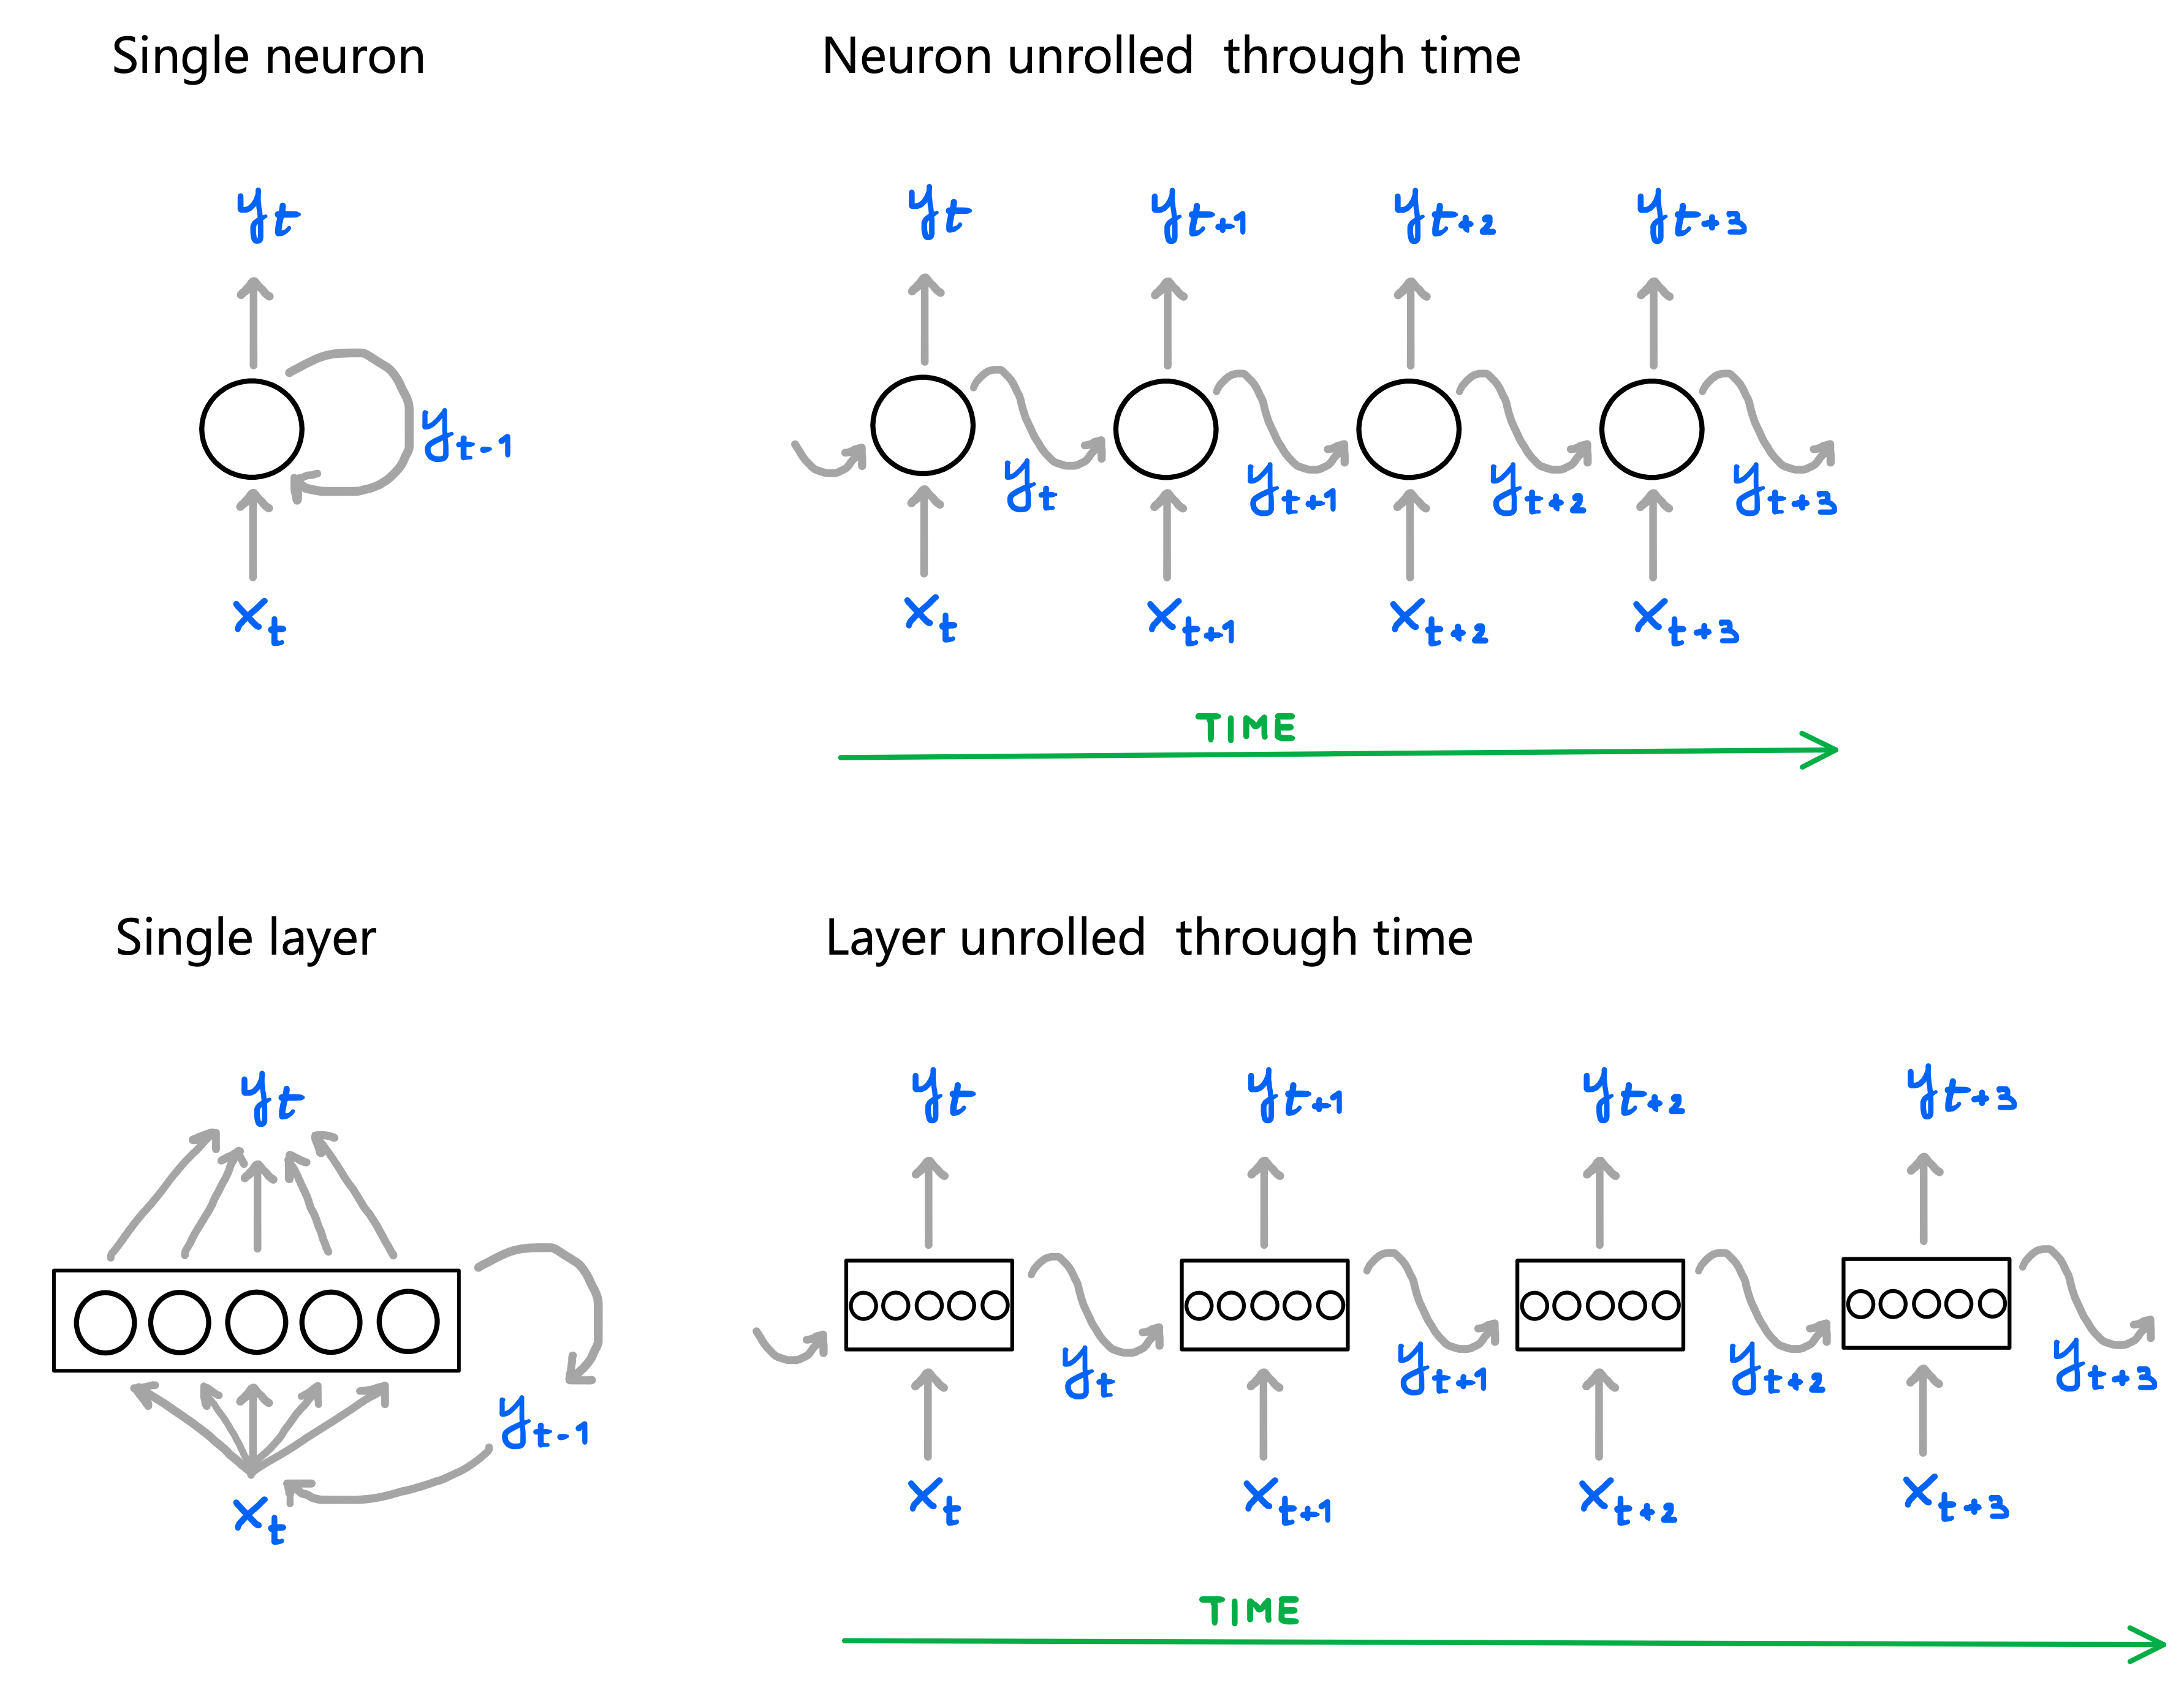
\includegraphics[width=1\textwidth]{nn_recurrent}
    \caption{Logic behind a recurrent neural network}
    \label{fig:nn_recurrent}
\end{figure}

Each recurrent neuron has two sets of weights, one for the inputs $x_t$ and the other for the previous output $y_{t-1}$. Naming $\mathbf{W}_x$ and $\mathbf{W}_y$ respectively these two sets of weights, we can rewrite the equation for the output $\mathbf{Y}_t$ of a recurrent layer:
\begin{align}
    \mathbf{Y}_t = \phi (\mathbf{X}_t \mathbf{W}_x + \mathbf{Y}_{t-1} \mathbf{W}_y + \mathbf{b})
\end{align}
where $\phi$ is the activation function of the layer and $\mathbf{b}$ is the bias. Concatenating the inputs $[\begin{array}{ll}{\mathbf{X}_t} & {\mathbf{Y}_{t-1}}\end{array}]$ and the weights $\mathbf{W} = \left[\begin{array}{c}{\mathbf{W}_x} \\ {\mathbf{W}_y}\end{array}\right]$, we can rewrite the equation as:
    \begin{align}
        \mathbf{Y}_t = \phi ([\begin{array}{ll}{\mathbf{X}_t} & {\mathbf{Y}_{t-1}}\end{array}] \mathbf{W} + \mathbf{b})
    \end{align}

We can say that the network is able to store some sort of "memory" of the past inputs and to use this information for the outputs of the the following time steps. A neuron, or layer of neurons, that is able to preserve some state across time steps is called a \textit{memory cell}. A cell's state at time $t$ can be denoted with $\mathbf{h}_t$, which corresponds to a function $\mathbf{h}_t = f(\mathbf{h}_{t-1}, \mathbf{x}_t)$. In the case of basic memory cells like the ones in a recurrent neural network, the element $\mathbf{h}_{t-1}$ corresponds exactly to the notation $\mathbf{y}_{t-1}$ that we used until now to denote the output from the previous time step.

The standard recurrent neural network model presents some drawbacks. First of all, when the network is trained on long sequences, it may suffer form the vanishing/exploding gradient problem, leading to convergence issues in the training procedure. Moreover, on the long run, the memory of information about the first time steps tends to fade away, since part of the information is lost at each step. We could consider the \acs{rnn} to have a short-term memory, which is not optimal when we need to predict events based on a long sequence of time steps. That is where the \acs{lstm} neural network comes in.


\subsection{\acs{lstm} neural network}
\paragraph{} An \acs{lstm} neural network, differently from a \acs{rnn}, is made of \textit{Long Short-Term Memory} (\acs{lstm}) cells \cite{NeuralComputation:lstm}. This type of cells allows the model to perform much better and to converge faster, in addition to preserving long-term information in long sequences. As shown in Figure \ref{fig:rnn_vs_lstm}, while the standard \acs{rnn} cell contains only a single computational unit (showed as a yellow box), the \acs{lstm} cell contains four interacting units (or layers), each one having a well-defined purpose. An \acs{lstm} cell keeps "in memory" two states, one for the short-term memory and the other for the long-term memory, respectively $\mathbf{h}_t$ and $\mathbf{C}_t$ (also called \textit{cell state}). The first one is the same that we saw for standard recurrent network's cells, while the cell state is what makes the \acs{lstm} model so special.
\begin{figure}[t]
    \centering
    \begin{subfigure}[t]{0.8\textwidth}
		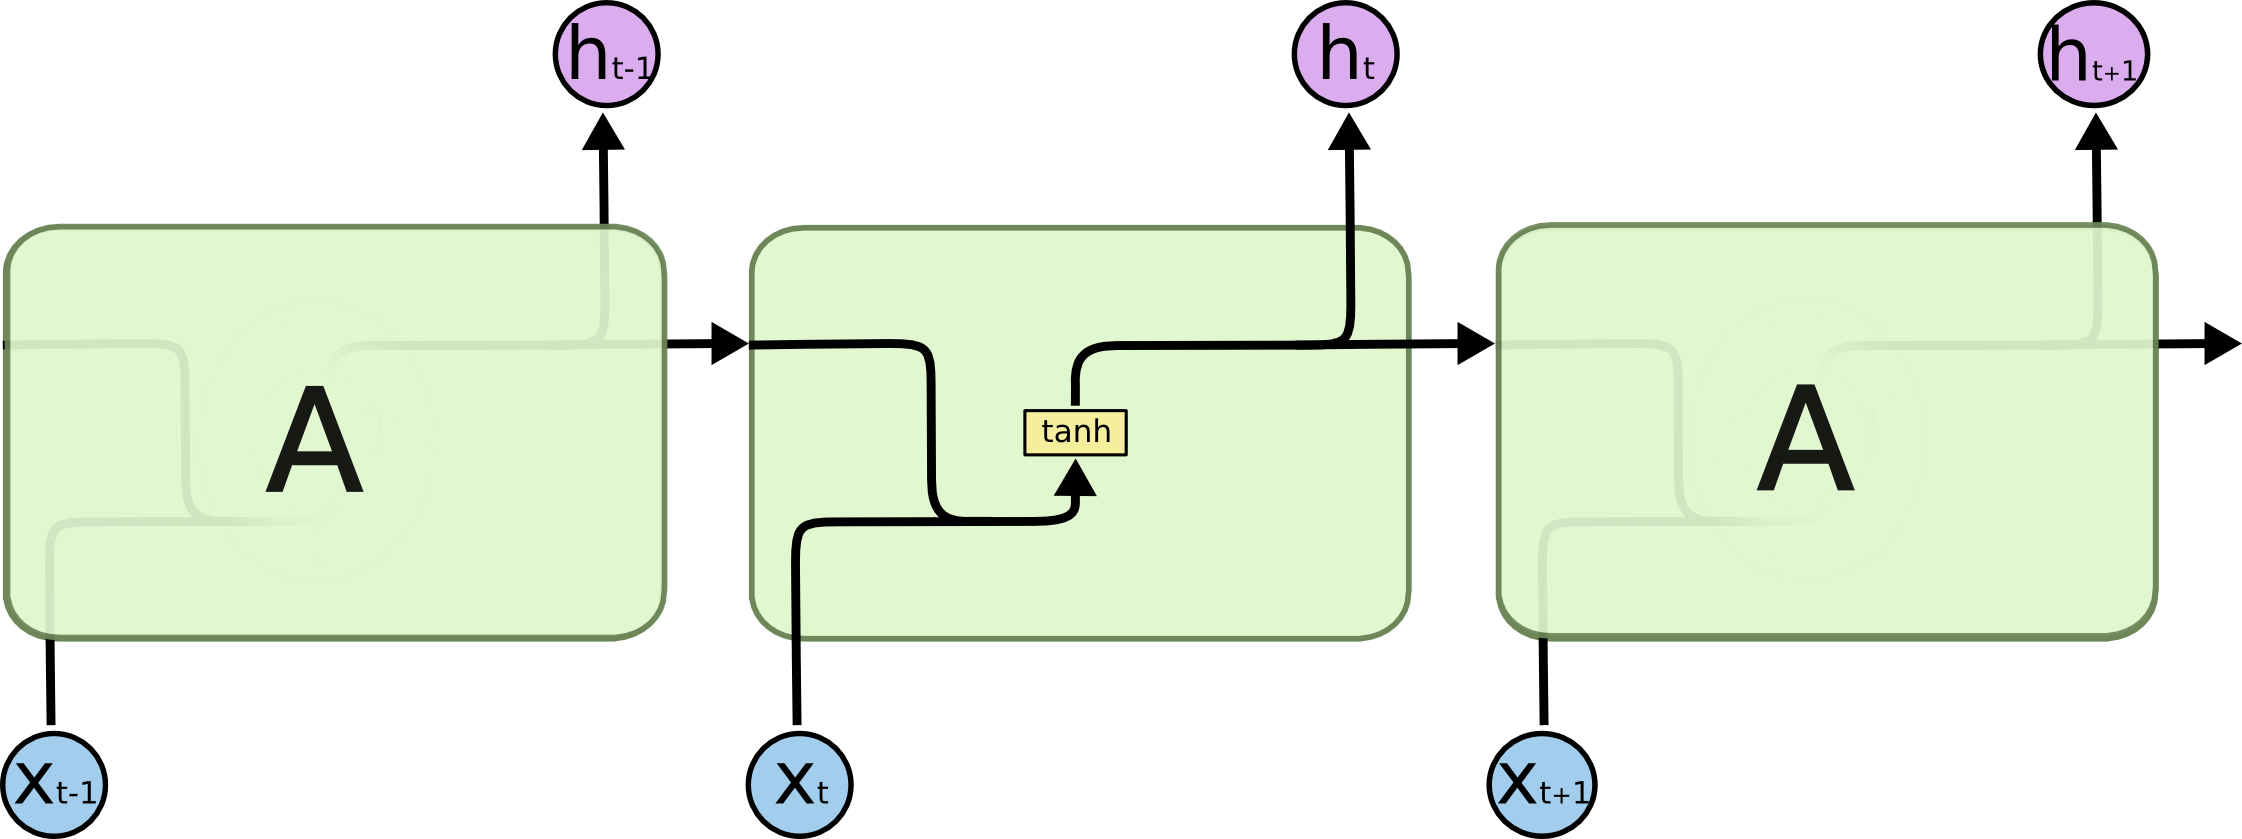
\includegraphics[width=1\textwidth]{nn_simplernn}
        \caption{Standard \acs{rnn} cell}
        \label{fig:nn_simplernn}
	\end{subfigure}
	~
	\begin{subfigure}[t]{0.8\textwidth}
		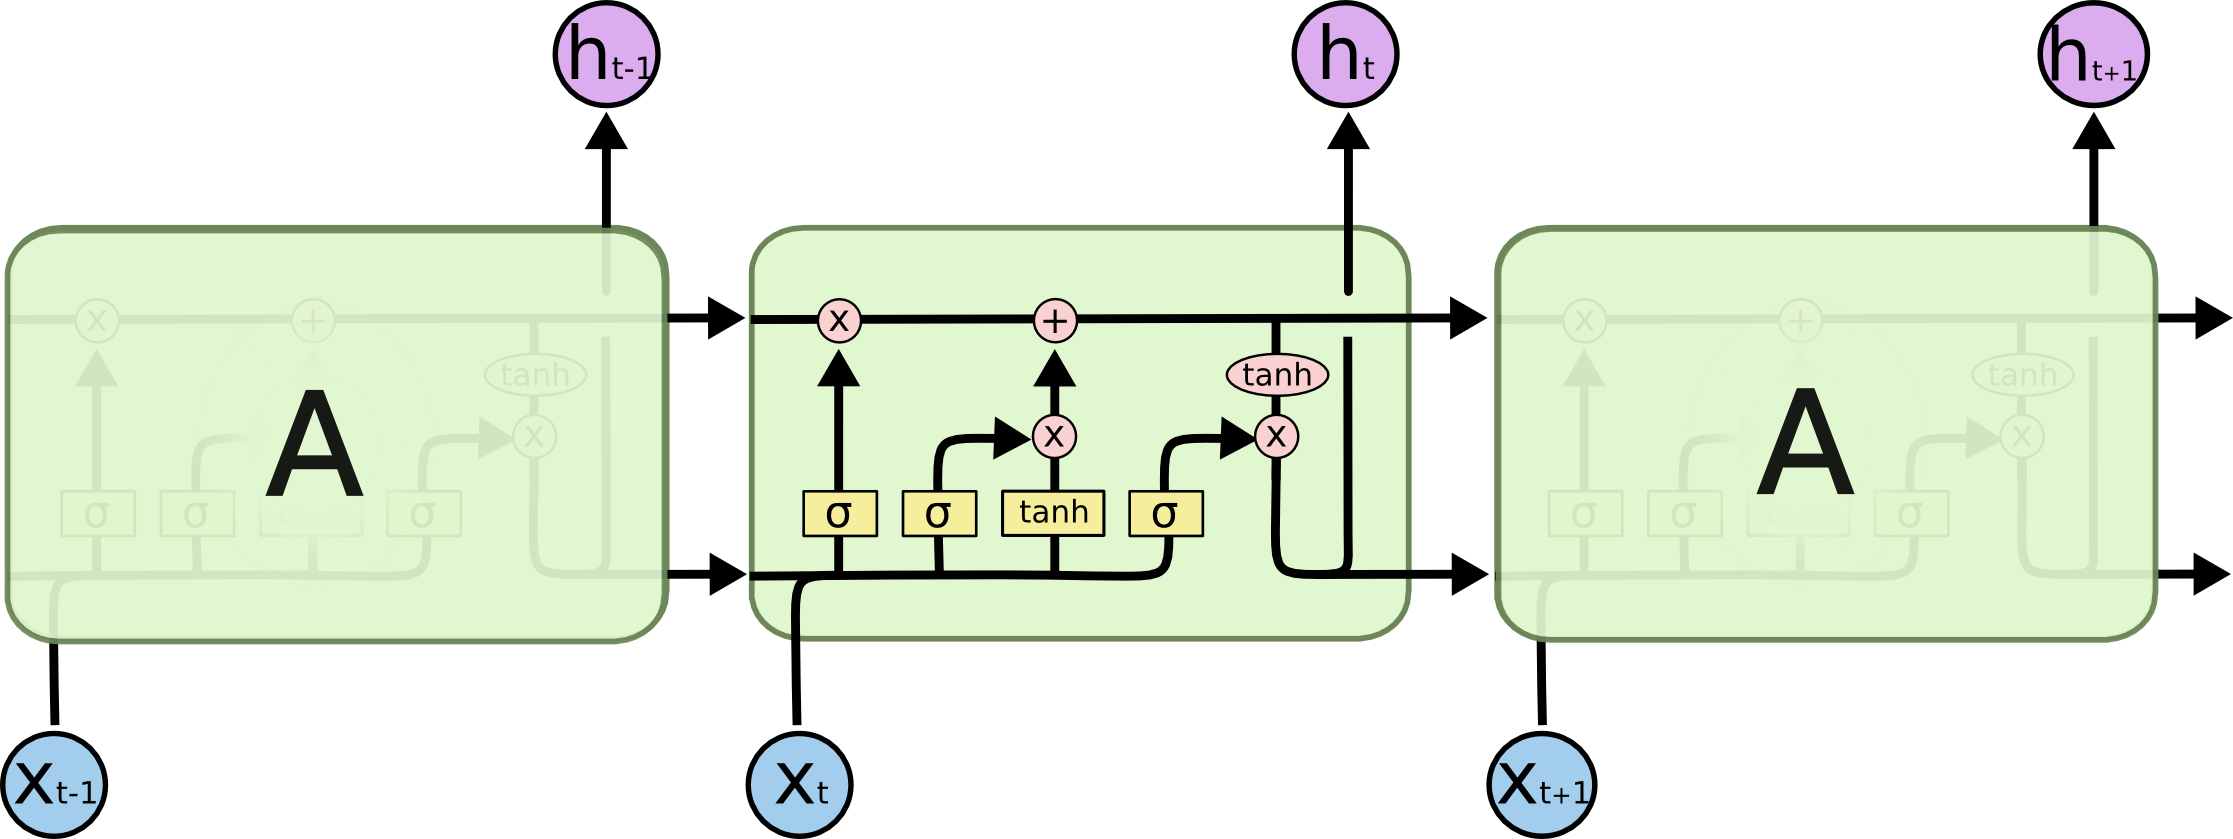
\includegraphics[width=1\textwidth]{nn_lstm}
        \caption{\acs{lstm} cell}
        \label{fig:nn_lstm}
    \end{subfigure}
    ~
    \begin{subfigure}[t]{0.6\textwidth}
		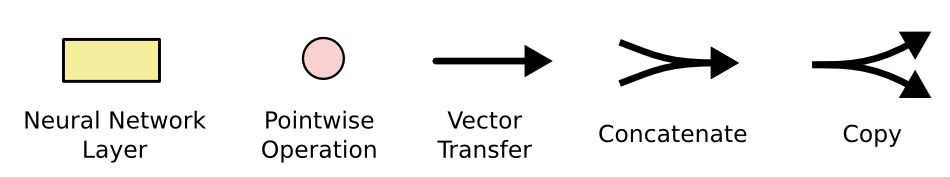
\includegraphics[width=1\textwidth]{nn_lstm_notation}
        \caption{Image notation}
        \label{fig:nn_lstm_notation}
	\end{subfigure}
    \caption{Difference between a standard \acs{rnn} cell and a \acs{lstm} cell (from \textit{colah's blog})}
    \label{fig:rnn_vs_lstm}
\end{figure}

In addition to the three inputs $\mathbf{x}_t$, $\mathbf{h}_{t-1}$ and $\mathbf{C}_{t-1}$, the \acs{lstm} cell makes use of four different fully connected layer, three of them using a sigmoid activation function and the remaining one using a \acs{tanh} activation function. Each one of the sigmoid activation outputs goes through a \textit{gate}, indicated in Figure \ref{fig:rnn_vs_lstm} with the symbol $\otimes$, representing an element-wise multiplication. Gates use the output of the sigmoids (between 0 and 1) to determine how much information should be let through. Let's dive into the functioning of an \acs{lstm} cell.

The cell state allows the network to decide what to store in the long-term memory and what to discard. Traversing the cell from left to right (Figure \ref{fig:nn_lstm_step1}), the cell states goes through two operations, the first being the \textit{forget gate} and the second being and addition operation. The forget state determines which long-term information to drop from $\mathbf{C}_{t-1}$ and it is controlled by the first sigmoid layer's output $f_t$, calculated from $\mathbf{x}_t$ and $\mathbf{h}_{t-1}$ (Figure \ref{fig:nn_lstm_step2}). The addition operation, on the other hand, adds information to the cell state based on the output of the \textit{input gate}, which determines which new information coming from $\mathbf{x}_t$ and $\mathbf{h}_{t-1}$ will be stored in the cell state (Figure \ref{fig:nn_lstm_step4}). The input gate is controlled by the second sigmoid layer's output $i_t$ and by the \acs{tanh} layer's output $\tilde{C}_t$ (Figure \ref{fig:nn_lstm_step3}). After that, the long-term state $\mathbf{C}_t$ is ready to be output, but before that, its state is copied to be passed to a \acs{tanh} activation function and to be filtered by the last gate, which is the \textit{output gate}, controlled by the third sigmoid layer's output $o_t$ (Figure \ref{fig:nn_lstm_step4}). This operation is essential in order to produce the short-term state $\mathbf{h}_t$ to output.

To sum up the fully-connected layer's roles:
\begin{itemize}
    \item The \acs{tanh} layer that outputs $\tilde{C}_t$ takes as inputs $\mathbf{x}_t$ and $\mathbf{h}_{t-1}$ and it is the same that we find in a basic recurrent cell. The result is partially stored as new information in the long-term state.
    \item The sigmoid layer that outputs $f_t$ takes as inputs $\mathbf{x}_t$ and $\mathbf{h}_{t-1}$ and it controls the forget gate. Based on the result, some parts of the long-term state are erased.
    \item The sigmoid layer that outputs $i_t$ takes as inputs $\mathbf{x}_t$ and $\mathbf{h}_{t-1}$ and it controls the input gate. Based on the result, some parts of the new information in $\tilde{C}_t$ are added to the long-term state.
    \item The sigmoid layer that outputs $o_t$ takes as inputs $\mathbf{x}_t$ and $\mathbf{h}_{t-1}$ and it controls the output gate. Based on the result, some parts of the long-term state are read and output as $\mathbf{h}_t$.
\end{itemize}
All the equations for the different outputs can be found in Figure \ref{fig:lstm_steps}.

Through this process, the \acs{lstm} model is able to preserve important information through time and to understand which are the essential inputs to keep and what to discard. This allows the network to learn long-term patterns in the data.
\newpage
\begin{figure}[H]
    \centering
    \begin{subfigure}[t]{0.7\textwidth}
		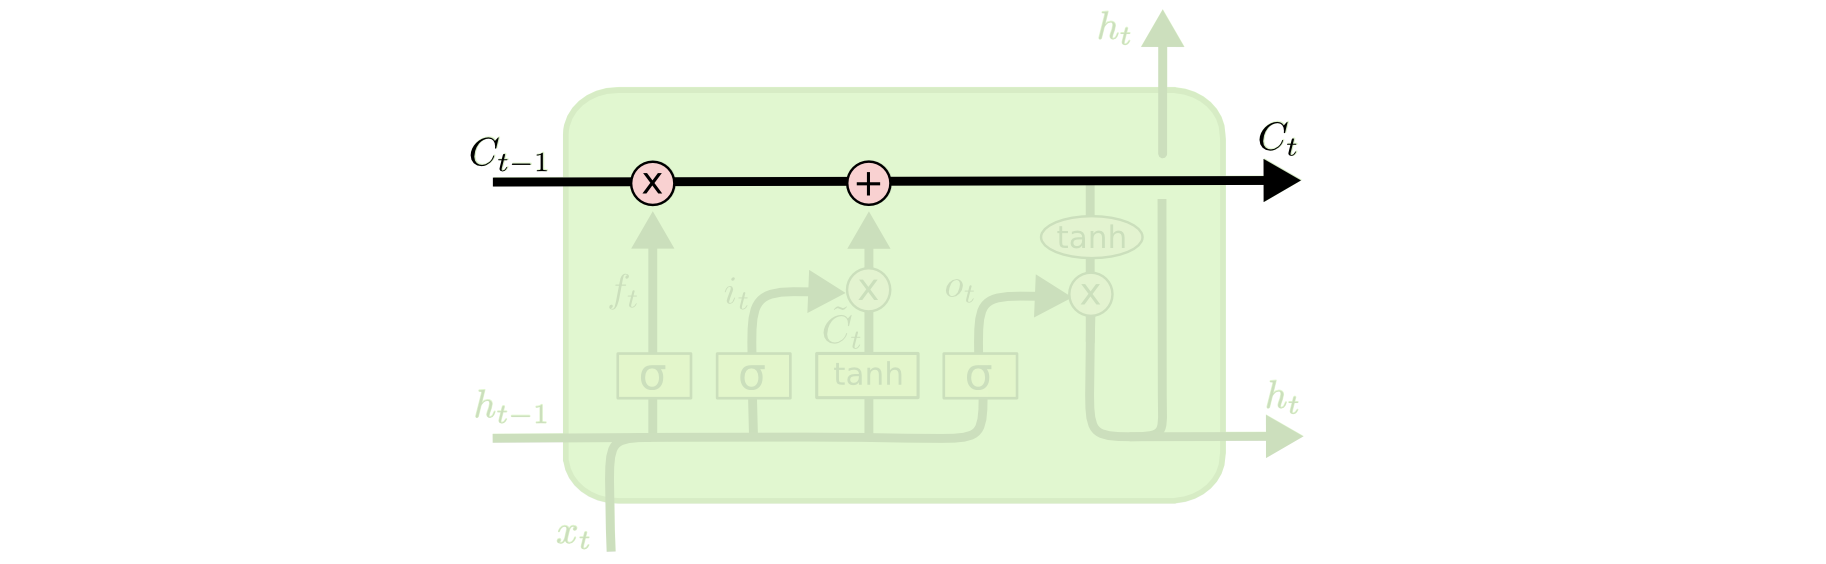
\includegraphics[width=1\textwidth]{nn_lstm_step1}
        \caption{}
        \label{fig:nn_lstm_step1}
	\end{subfigure}
	~
	\begin{subfigure}[t]{0.7\textwidth}
		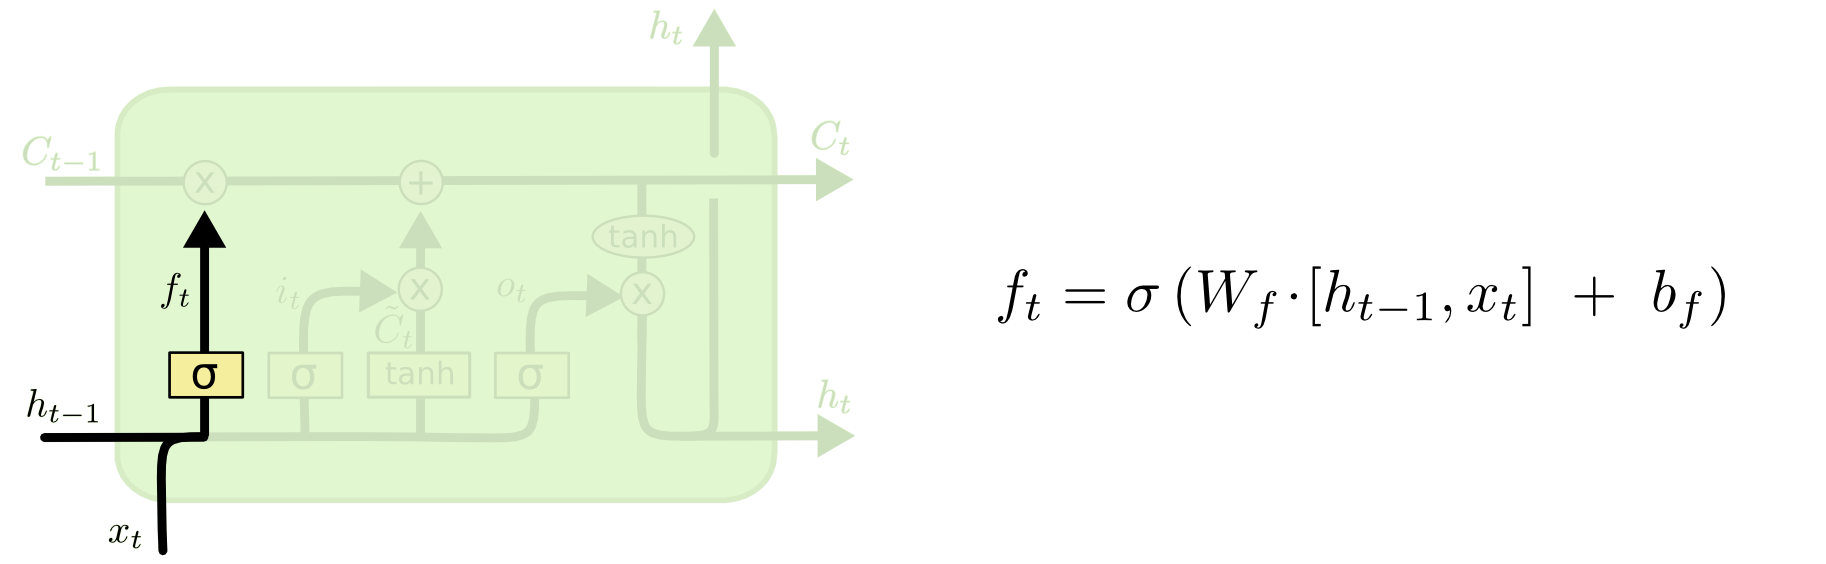
\includegraphics[width=1\textwidth]{nn_lstm_step2}
        \caption{}
        \label{fig:nn_lstm_step2}
    \end{subfigure}
    ~
    \begin{subfigure}[t]{0.7\textwidth}
		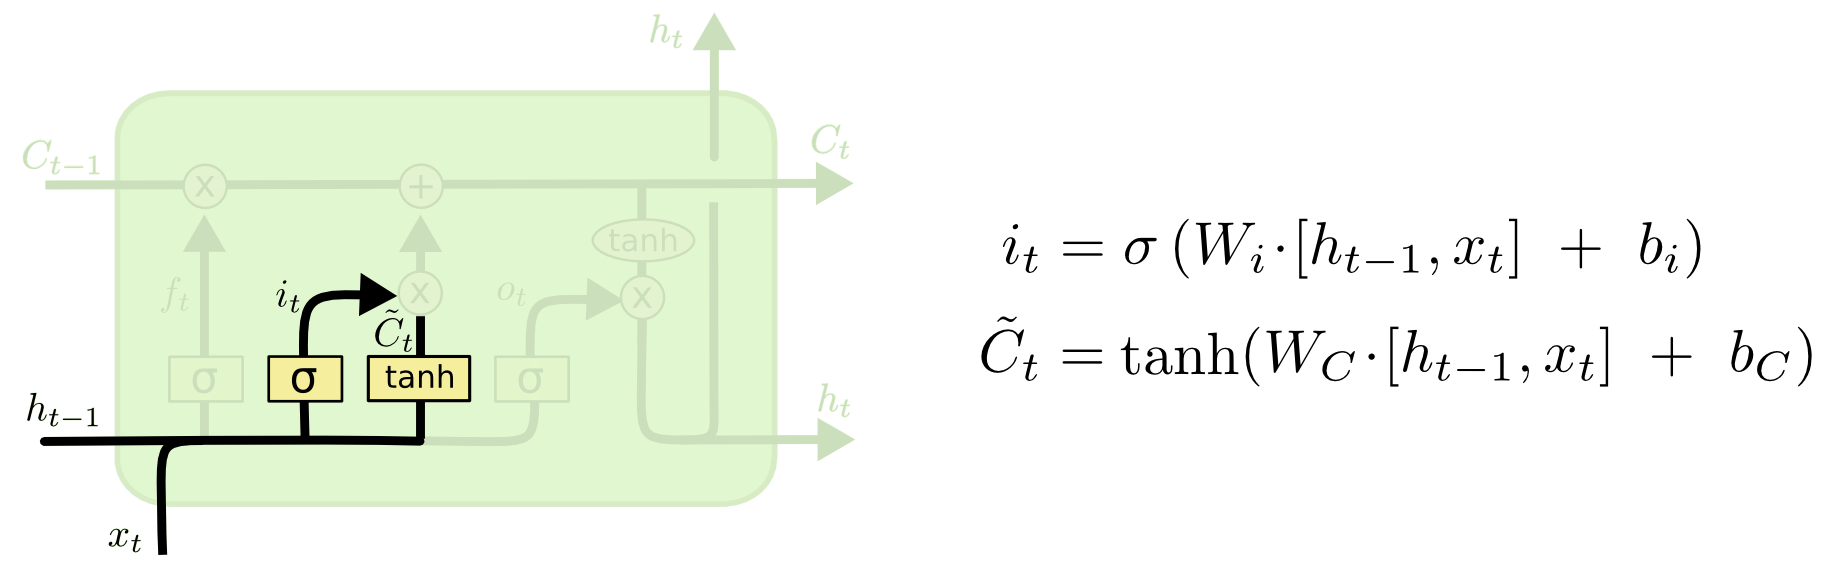
\includegraphics[width=1\textwidth]{nn_lstm_step3}
        \caption{}
        \label{fig:nn_lstm_step3}
    \end{subfigure}
    ~
    \begin{subfigure}[t]{0.7\textwidth}
		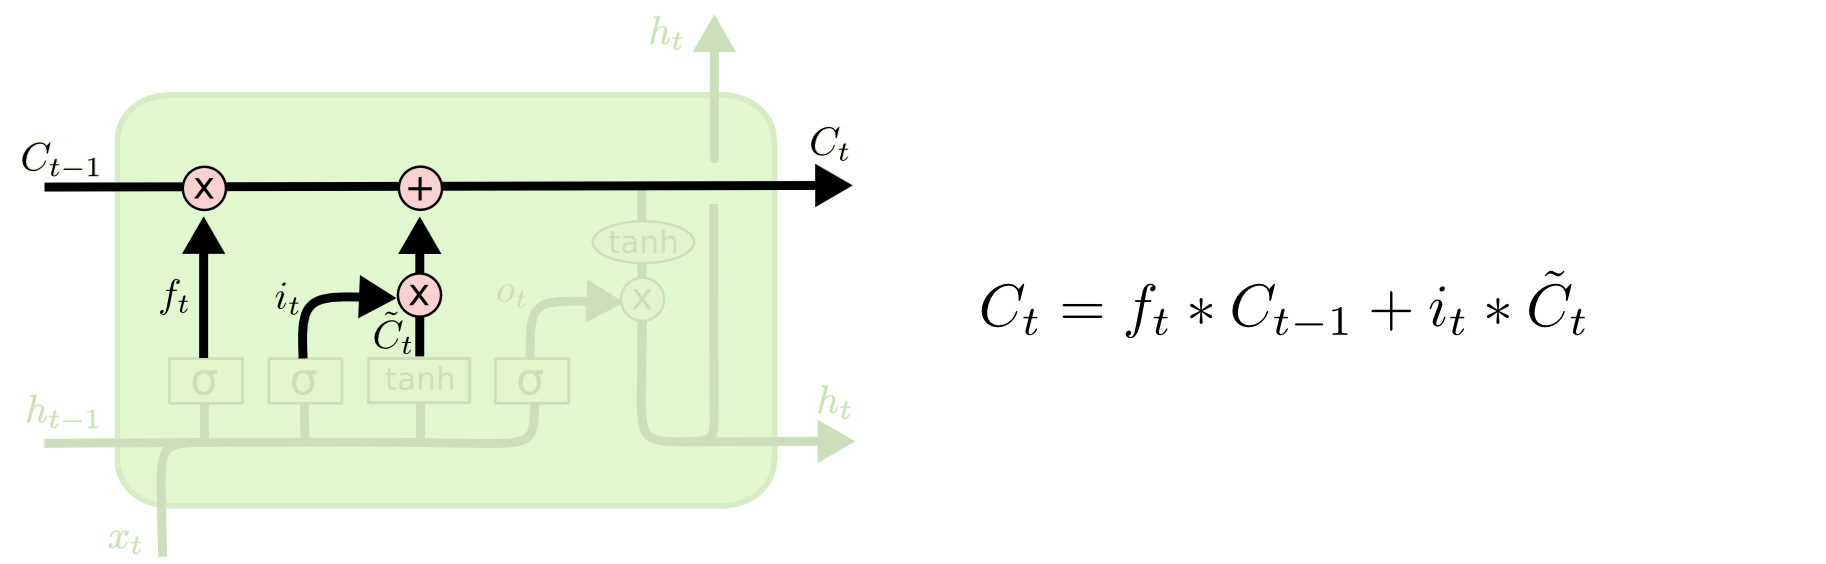
\includegraphics[width=1\textwidth]{nn_lstm_step4}
        \caption{}
        \label{fig:nn_lstm_step4}
    \end{subfigure}
    ~
    \begin{subfigure}[t]{0.7\textwidth}
		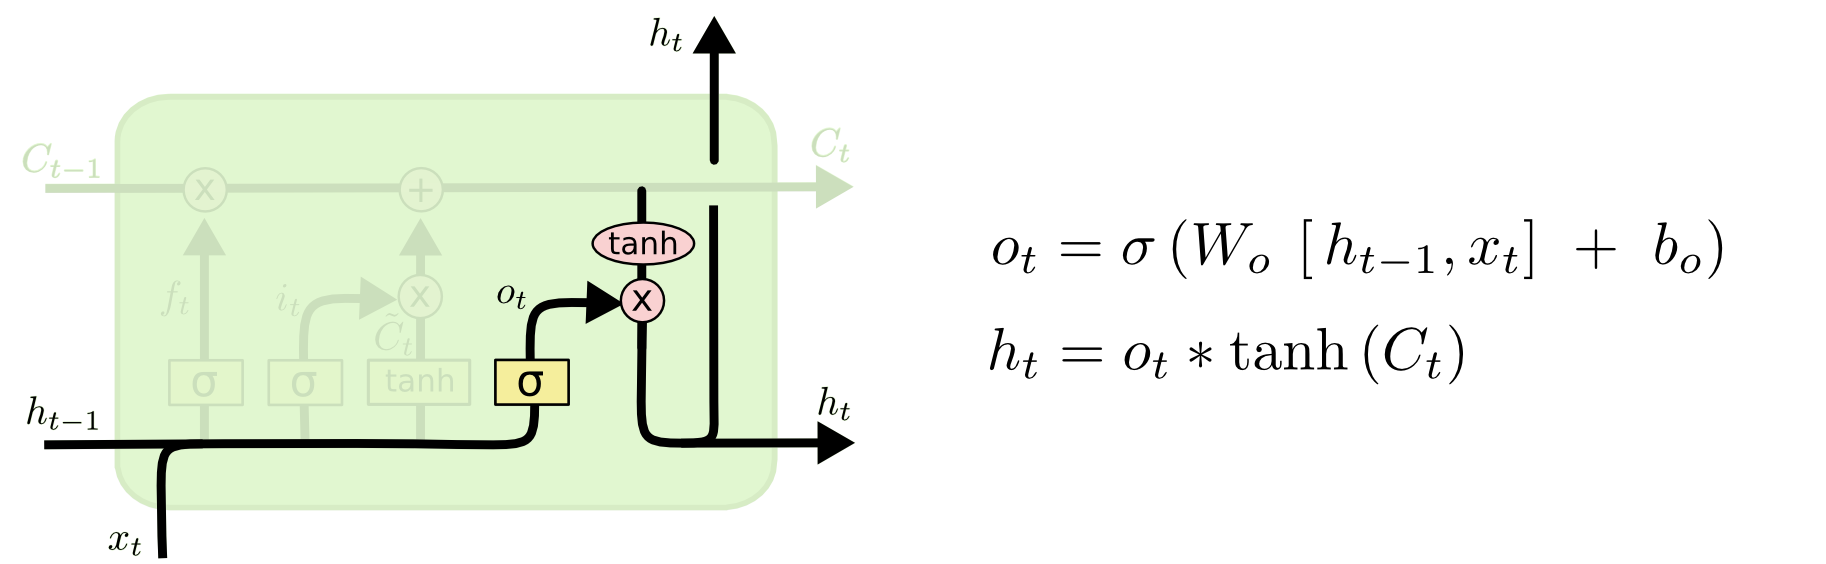
\includegraphics[width=1\textwidth]{nn_lstm_step5}
        \caption{}
        \label{fig:nn_lstm_step5}
    \end{subfigure}
    \caption{Elements in an \acs{lstm} cell step-by-step (from \textit{colah's blog})}
    \label{fig:lstm_steps}
\end{figure}
\newpage

%--------------------------------------------------
% Functional connectivity and graph representation
%--------------------------------------------------

\section{Functional connectivity and graph representation} \label{sec: fc_graphs}
\paragraph{} This section explains some basic knowledge about the functional connectivity of the brain activity and its convenient representation using graphs, which has led to the use of graph-based deep learning models.

Functional connectivity represents the presence of statistical dependencies between the time series of different brain regions \cite{NeurobiologyLanguage:functionalconnectivity}. In other words, functional connectivity measures the relations between time windows of brain activity in different areas of the brain. Assuming that the data respect Gaussian assumptions, these dependencies are usually expressed using covariance or correlation.

In the case of functional \acs{eeg} connectivity, the signal of an electrode represents the brain activity of the brain region in which the electrode is located. We can obtain a sequence of time windows for each brain region's activity by temporally segmenting the signal generated by the electrode located in that region. For instance, if we want to determine the functional connectivity of two brain regions, represented by the electrodes $a_1$ and $a_2$ respectively, we consider their time series $t_{a_1}$ and $t_{a_2}$ and we can compute the Pearson correlation coefficient of the two time series:
\begin{align}
    \textit{corr}_{t_{a_1} t_{a_2}} = \frac{\textit{cov}_{t_{a_1} t_{a_2}}}{\textit{sd}_{t_{a_1}} \cdot \textit{sd}_{t_{a_2}}}
\end{align}
where $\textit{cov}_{t_{a_1} t_{a_2}}$ is the covariance and $\textit{sd}_{t_{a_1}}$ and $\textit{sd}_{t_{a_2}}$ are the standard deviations of the two time series.

Brain's functional connectivity can be properly represented through graphs. A graph is a data structure consisting of nodes and edges. The nodes are entities that hold some sort of information, while the edges are the connections between nodes and they can hold information too. Usually the information held by an edge refer to the relation between the nodes connected by that edge. Graphs are useful to represent non-euclidean data and they can have several properties limiting their flexibility to certain constraints.

In computer science, we can represent a graph with three matrices:
\begin{itemize}
    \item Binary adjacency matrix $\mathbf{A} \in\{0,1\}^{N \times N}$
    \item Node attributes matrix $\mathbf{X} \in \mathbb{R}^{N \times F}$
    \item Edge attributes matrix $\mathbf{E} \in \mathbb{R}^{N \times N \times S}$
\end{itemize}
where $N$ is the number of nodes, $F$ is the number of features for each node and $S$ is the number of edges. The adjacency matrix $\mathbf{A}$ shows the connections between the nodes: the cell at row $i$ and column $j$ contains 1 if there is an edge connecting nodes $i$ and $j$ and it contains 0 otherwise. The node attributes matrix $\mathbf{X}$ contains a row of $F$ features for each node. The edge attributes matrix $\mathbf{E}$ is similar to the adjacency matrix, but instead of containing only ones and zeros, it stores the $S$ attributes of each edge across the third dimension.

A variation of the adjacency matrix is the adjacency matrix with inserted self-loops:
\begin{align*}
    \hat{\mathbf{A}} = \mathbf{A} + \mathbf{I}_N
\end{align*}
where $\mathbf{I}_N$ is an $N \times N$ identity matrix, that is a square matrix with ones on the main diagonal and zeros elsewhere. Another important matrix representing graphs is the degree matrix $\mathbf{D}$, which is a diagonal matrix where each value of the diagonal is the degree of its corresponding node. The degree is the sum of each row of the adjacency matrix.

Functional connectivity can be expressed as a graph by considering each electrode (brain region) as a node and by using the correlation value between electrodes as the attribute of the edges between nodes. In this case, we would obtain a graph having a node for each electrode and an edge for each couple of nodes. In order to reduce the number of edges, we could keep only the most significative ones, that are the ones whose correlation's absolute value is near 1. This representation is able to express the statistical dependencies between brain regions just for a given time instant. In order to introduce the time dimension, we can generate a new graph for each time window, obtaining a sequence of different graphs (see Figure \ref{fig:graph_sequence}). Through this representation, we can see the evolution of brain region dependencies across time, with edges appearing or disappearing based on the correlation value in that time step.
\begin{figure}[htbp]
    \centering
    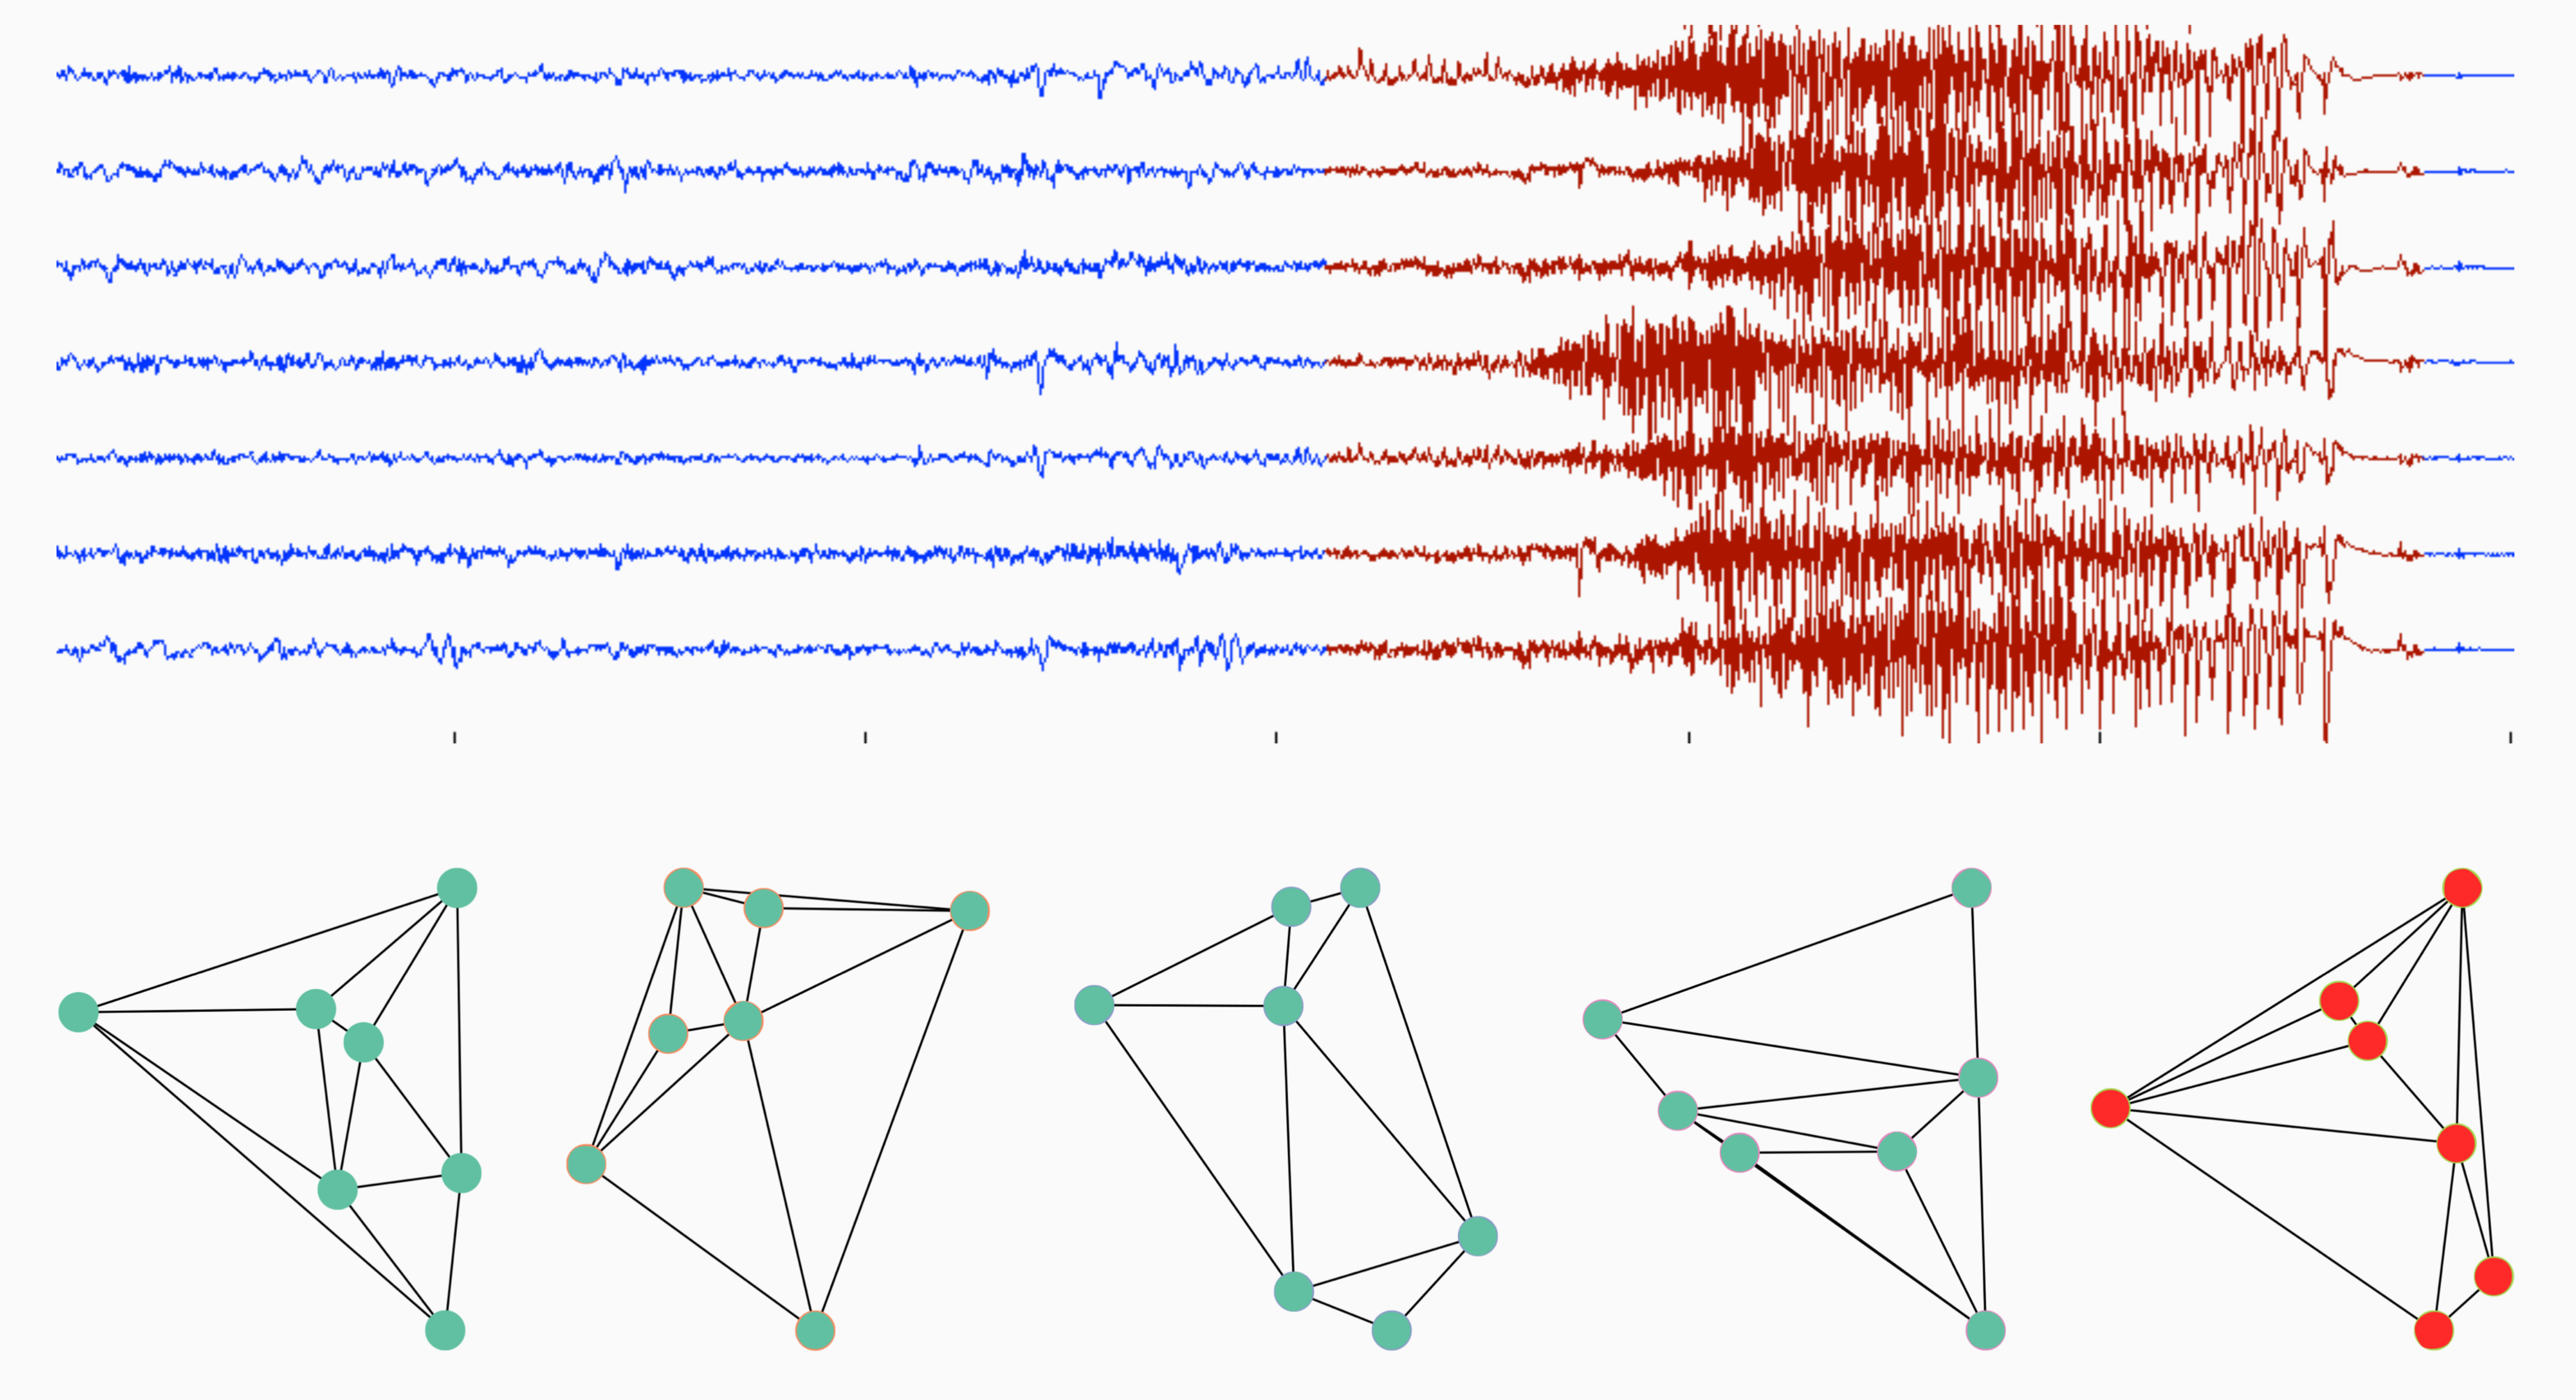
\includegraphics[width=0.8\textwidth]{graph_sequence}
    \caption{Sequence of graphs representing the functional connectivity (from \cite{arXiv:graphstream})}
    \label{fig:graph_sequence}
\end{figure}

%--------------------------------------------------
% Graph-based deep learning models
%--------------------------------------------------

\section{Graph-based deep learning models} \label{sec: graph_dl}
\paragraph{} Geometric deep learning stems from the need to apply deep learning models to non-euclidean data. A lot of research on this topic has been conducted during the last decades in order to develop suitable models for this purpose. One of the most common examples of non-euclidean data is the graph data structure, which is able to encode information about the structure and the relation between entities, while still representing individual features. In order to deal with graph data, graph neural networks (\acsp{gnn}) have been created.

\subsection{Graph neural network and graph convolution} Graph neural networks (\acsp{gnn}) are deep learning models dedicated to working with graph-structured data. They are able to learn from graph information like structure, relationship, connections and individual features of the entities. Their flexibility opens the door to a wide new range of real-world applications, whose data require to take into account the structural information.

One of the most interesting approach to the application of neural networks to graph is the \textit{graph convolution}, which tries to generalize convolutional layers to arbitrary neighbours. The more standard version of convolutional neural networks, indeed, are generally applied to images, where the neighbourhood is determined by the location of the pixels in a 2D space. However, there are situation in which the spatial information is not available and we have to rely on connection between entities in order to define a neighbourhood (just think of molecules or social networks). This is exactly what graph convolution tries to achieve. In graph convolution, the output of a layer is described by the following equation (expressed in matrix form):
\begin{align}
    \mathbf{X}^{(out)}=\phi\left(\tilde{\mathbf{A}} \mathbf{X}^{(in)} \mathbf{W} + \mathbf{b}\right)
\end{align}
where $\phi$ is the activation function, $\mathbf{b}$ is the bias, $\mathbf{W}$ is the matrix of model's weights, $\mathbf{X}$ is the node attribute matrix and $\tilde{\mathbf{A}}$ is a modified version of the adjacency matrix that can be computed in different ways. The presence of the adjacency matrix (or some modified version) multiplied to the node features matrix allows the network to filter the features. In this way, the processing of a feature node is influenced only by the neighbourhood's features, determined by the nodes connected to it.

Among the most known geometric deep learning models, there is the \acf{gcn}, from the paper by Kipf and Welling (\cite{arXiv:gcn}). The paper presents a spectral convolutional model applied to graph learning. In a \acs{gcn}, the output of a layer is defined as:
\begin{align}
    \mathbf{X}^{(out)}=\phi\left(\hat{\mathbf{D}}^{-\frac{1}{2}} \hat{\mathbf{A}} \hat{\mathbf{D}}^{-\frac{1}{2}} \mathbf{X}^{(in)} \mathbf{W} + \mathbf{b}\right)
\end{align}
so in this case, $\tilde{\mathbf{A}}$ is computed as $\tilde{\mathbf{A}} = \hat{\mathbf{D}}^{-\frac{1}{2}} \hat{\mathbf{A}} \hat{\mathbf{D}}^{-\frac{1}{2}}$. In the equation, $\hat{\mathbf{A}}$ is the adjacency matrix with inserted self-loops, while $\hat{\mathbf{D}}$ is the degree matrix computed from $\hat{\mathbf{A}}$. The $\hat{\mathbf{D}}$ are to the power of $-\frac{1}{2}$ for renormalization reasons.

\subsection{Edge-conditioned convolution}
\paragraph{} The graph convolution is able to filter the node features based on the adjacency matrix, but it doesn't take into account the edge attributes matrix. The \textit{edge-conditioned convolution} (\acs{ecc}) address this issue by replacing the model's weights with a neural network that transforms the edge features into convolutional kernels (\cite{arXiv:eccn}). The resulting formula for a single node is:
\begin{align}
    \mathbf{X}^{(out)}_i=\phi\left(\frac{1}{\mathcal{N}(i)} \sum_{j \in \mathcal{N}(i)} \mathbf{X}^{(in)}_j f(\mathbf{E}_{ji}) + \mathbf{b}\right)
\end{align}
where $\mathcal{N}(i)$ are the one-step neighbourhood of node $i$, $\mathbf{E}$ is the edge attributes matrix and $f(\cdot)$ is a dense neural network that output the convolution kernel as a function of $\mathbf{E}$.

\subsection{Global pooling}
\paragraph{} Like in standard convolutional neural networks, the convolution on graph is usually followed by a pooling layer to get more general features. The problem with the generalization of local pooling layer is that in graph there is no locality as in images. For this reason, the most common approach is to use a global pooling layer on the graph's node features, which reduces the representation of the graph to a single "virtual" node that summarizes all the features of all the original nodes in the graph. This is usually placed after all the convolutional layer, just before the dense neural network for the final prediction.

A global pooling layer aggregates all the node features through an aggregation function (i.e. mean, sum, max functions). For this project, global average pooling has been used, which is defined as:
\begin{align}
    out^{(l)} = \frac{1}{N^{(l)}} \sum_{i=1}^{N^{(l)}} \mathbf{X}^{(l)}_i
\end{align}

The downside of this approach is that, while summarizing the node features, the global pooling layer isn’t able to preserve the graph’s topological information. In order to take into account also the structure of the graph, hierarchical pooling layers have been proposed lately. They are able to coarsens the graph by dropping some of its nodes based on a measure of the importance of the nodes, thus down-sampling the graph representation.

\subsection{Graph-based LSTM and convolutional neural networks}
\paragraph{} For the purpose of this project, graph convolution has been used as a preprocessing tool in order to extract features from the graph data. The graph-conv-pool block, composed by a graph convolutional layer and a global pooling layer, can be followed by any standard neural network, such as dense, convolutional and \acs{lstm} neural networks. With this configuration, the role of the graph-conv-pool block is simply to deal with the graph structure of the data and to extract structural features in a form that is processable for standard models.

\section{State-of-the-art in seizure prediction}